%-------------------------------------------------------------------------------
% This file provides a skeleton ATLAS paper.
%-------------------------------------------------------------------------------
% \pdfoutput=1
% The \pdfoutput command is needed by arXiv/JHEP/JINST to ensure use of pdflatex.
% It should be included in the first 5 lines of the file.
% \pdfinclusioncopyfonts=1
% This command may be needed in order to get \ell in PDF plots to appear. Found in
% https://tex.stackexchange.com/questions/322010/pdflatex-glyph-undefined-symbols-disappear-from-included-pdf
%-------------------------------------------------------------------------------
% Specify where ATLAS LaTeX style files can be found.
\newcommand*{\ATLASLATEXPATH}{latex/}
% Use this variant if the files are in a central location, e.g. $HOME/texmf.
% \newcommand*{\ATLASLATEXPATH}{}
%-------------------------------------------------------------------------------
\documentclass[PUB, atlasdraft=true, texlive=2017, UKenglish]{\ATLASLATEXPATH atlasdoc}
% The language of the document must be set: usually UKenglish or USenglish.
% british and american also work!
% Commonly used options:
%  atlasdraft=true|false This document is an ATLAS draft.
%  texlive=YYYY          Specify TeX Live version (2016 is default).
%  coverpage             Create ATLAS draft cover page for collaboration circulation.
%                        See atlas-draft-cover.tex for a list of variables that should be defined.
%  cernpreprint          Create front page for a CERN preprint.
%                        See atlas-preprint-cover.tex for a list of variables that should be defined.
%  NOTE                  The document is an ATLAS note (draft).
%  PAPER                 The document is an ATLAS paper (draft).
%  CONF                  The document is a CONF note (draft).
%  PUB                   The document is a PUB note (draft).
%  BOOK                  The document is of book form, like an LOI or TDR (draft)
%  txfonts=true|false    Use txfonts rather than the default newtx
%  paper=a4|letter       Set paper size to A4 (default) or letter.

%-------------------------------------------------------------------------------
% Extra packages:
\usepackage{\ATLASLATEXPATH atlaspackage}
% Commonly used options:
%  biblatex=true|false   Use biblatex (default) or bibtex for the bibliography.
%  backend=bibtex        Use the bibtex backend rather than biber.
%  subfigure|subfig|subcaption  to use one of these packages for figures in figures.
%  minimal               Minimal set of packages.
%  default               Standard set of packages.
%  full                  Full set of packages.
%-------------------------------------------------------------------------------
% Style file with biblatex options for ATLAS documents.
\usepackage{\ATLASLATEXPATH atlasbiblatex}

% Useful macros
\usepackage{\ATLASLATEXPATH atlasphysics}
% See doc/atlas_physics.pdf for a list of the defined symbols.
% Default options are:
%   true:  journal, misc, particle, unit, xref
%   false: BSM, heppparticle, hepprocess, hion, jetetmiss, math, process,
%          other, snippets, texmf
% See the package for details on the options.

% Files with references for use with biblatex.
% Note that biber gives an error if it finds empty bib files.
% \addbibresource{tthbkgpubnote.bib}
\addbibresource{bib/ATLAS.bib}
\addbibresource{bib/CMS.bib}
\addbibresource{bib/ConfNotes.bib}
\addbibresource{bib/PubNotes.bib}

\addbibresource{bib/ttw.bib}
\addbibresource{bib/ttbb.bib}

% Paths for figures - do not forget the / at the end of the directory name.
\graphicspath{{logos/}{figures/}}

% Add you own definitions here (file tthbkgpubnote-defs.sty).
\usepackage{tthbkgpubnote-defs}

%-------------------------------------------------------------------------------
% Generic document information
%-------------------------------------------------------------------------------

% Title, abstract and document 
%-------------------------------------------------------------------------------
% This file contains the title, author and abstract.
% It also contains all relevant document numbers used by the different cover pages.
%-------------------------------------------------------------------------------

% Title
\AtlasTitle{Study of $t\bar{t}b\bar{b}$ and $t\bar{t}W$ background modelling for  $t\bar{t}H$ analyses}

% Draft version:
% Should be 1.0 for the first circulation, and 2.0 for the second circulation.
% If given, adds draft version on front page, a 'DRAFT' box on top of each other page, 
% and line numbers.
% Comment or remove in final version.
\AtlasVersion{1.0}

% Abstract - % directly after { is important for correct indentation
\AtlasAbstract{%
This note presents Monte Carlo generator comparisons of the $t\bar{t}b\bar{b}$ and $t\bar{t}W$  processes at particle level. The aim is to compare the modelling of some important backgrounds to $t\bar{t}H$ measurements in the Higgs to $b\bar{b}$ and Higgs to multi-lepton decay channels and the treatment of the associated theory uncertainties for a full Run-2 ATLAS+CMS combination. As a first step, pre-fit modelling and theory uncertainties as used in the experiments are compared in the relevant analysis regions.%Observables which are expected to be sensitive to differences in the generators or sensitive to the signal versus background discrimination in the respective ttH(bb) or ttH(multi-lepton) analyses are shown.
}

% Author - this does not work with revtex (add it after \begin{document})
% This has to be commented out for TDR etc.
% \author{The ATLAS Collaboration}

% ATLAS reference code, to help ATLAS members to locate the paper
\AtlasRefCode{HIGG-2019-19}

% CERN preprint number
% \PreprintIdNumber{CERN-EP-2019-XX}

% ATLAS date - arXiv submission; usually filled in by the Physics Office
% \AtlasDate{\today}

% ATLAS heading - heading at top of title page. Set for TDR etc.
% \AtlasHeading{ATLAS ABC TDR}

% arXiv identifier
% \arXivId{14XX.YYYY}

% HepData record
% \HepDataRecord{ZZZZZZZZ}

% Submission journal and final reference
% \AtlasJournal{Phys.\ Lett.\ B.}
% \AtlasJournalRef{\PLB 789 (2017) 123}
% \AtlasDOI{}

%-------------------------------------------------------------------------------
% The following information is needed for the cover page. The commands are only defined
% if you use the coverpage option in atlasdoc or use the atlascover package
%-------------------------------------------------------------------------------

% List of supporting notes  (leave as null \AtlasCoverSupportingNote{} if you want to skip this option)
% \AtlasCoverSupportingNote{Short title note 1}{https://cds.cern.ch/record/XXXXXXX}
% \AtlasCoverSupportingNote{Short title note 2}{https://cds.cern.ch/record/YYYYYYY}
%
% OR (the 2nd option is deprecated, especially for CONF and PUB notes)
%
% Supporting material TWiki page  (leave as null \AtlasCoverTwikiURL{} if you want to skip this option)
% \AtlasCoverTwikiURL{https://twiki.cern.ch/twiki/bin/view/Atlas/WebHome}

% Comment deadline
 \AtlasCoverCommentsDeadline{14 October 2019}
%
% Analysis team members - contact editors should no longer be specified
% as there is a generic email list name for the editors
% \AtlasCoverAnalysisTeam{Peter Analyser, Susan Editor1, Jenny Editor2, Alphonse Physicien}
\AtlasCoverAnalysisTeam{Paul Glaysher, Kirill Grevtsov, Judith Katzy}

% Editorial Board Members - indicate the Chair by a (chair) after his/her name
% Give either all members at once (then they appear on one line), or separately
% \AtlasCoverEdBoardMember{EdBoard~Chair~(chair), EB~Member~1, EB~Member~2, EB~Member~3}
% \AtlasCoverEdBoardMember{EdBoard~Chair~(chair)}
% \AtlasCoverEdBoardMember{EB~Member~1}
% \AtlasCoverEdBoardMember{EB~Member~2}
% \AtlasCoverEdBoardMember{EB~Member~3}

% A PUB note has readers and not an EdBoard -- give their names here (one line or several entries)
\AtlasCoverReaderMember{Klaus Moenig, Stephane Willocq}
% \AtlasCoverReaderMember{Reader~1}
% \AtlasCoverEdBoardMember{Reader~2}

% Editors egroup
% \AtlasCoverEgroupEditors{atlas-GROUP-2019-XX-editors@cern.ch}

% EdBoard egroup
% \AtlasCoverEgroupEdBoard{atlas-GROUP-2019-XX-editorial-board@cern.ch}


% Author and title for the PDF file
\hypersetup{pdftitle={ATLAS document},pdfauthor={The ATLAS Collaboration}}

%-------------------------------------------------------------------------------
% Content
%-------------------------------------------------------------------------------
\begin{document}

\maketitle

\tableofcontents

\clearpage
\section{Introduction}
\label{sec:intro}

\begin{figure}[!htb]
\centering
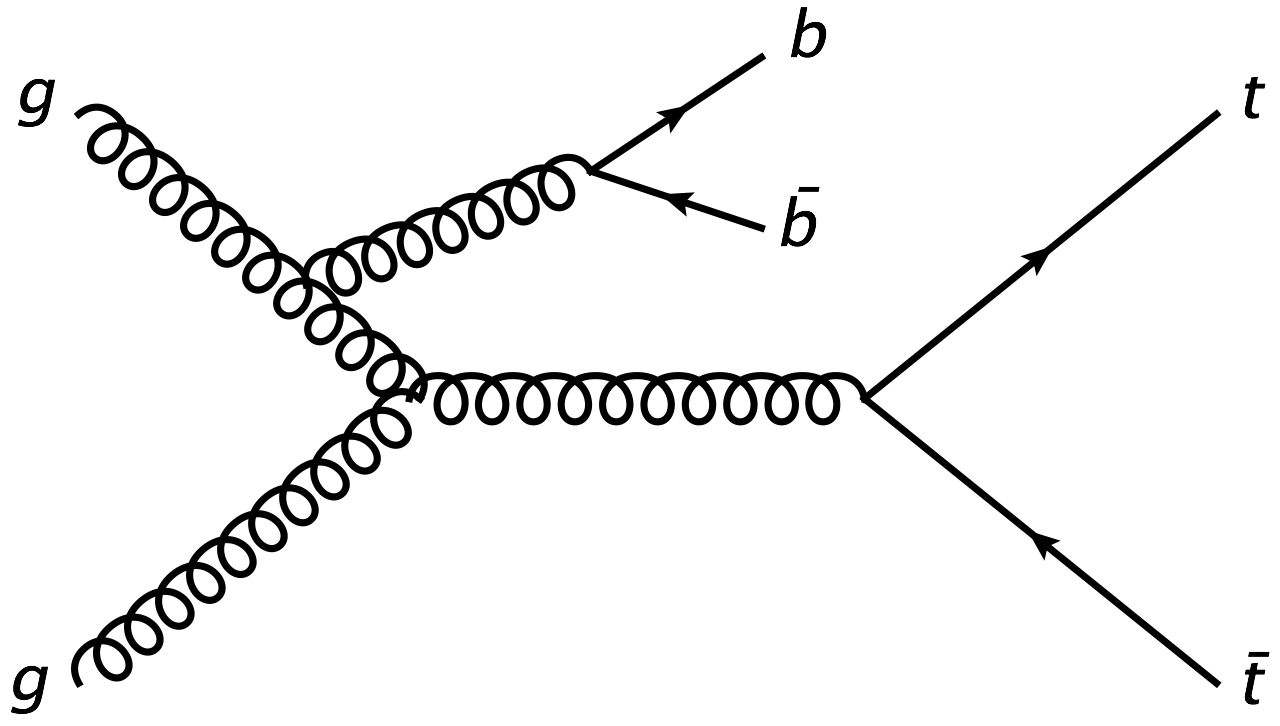
\includegraphics[width=0.35\textwidth]{Plots/ttbb/ttbb}
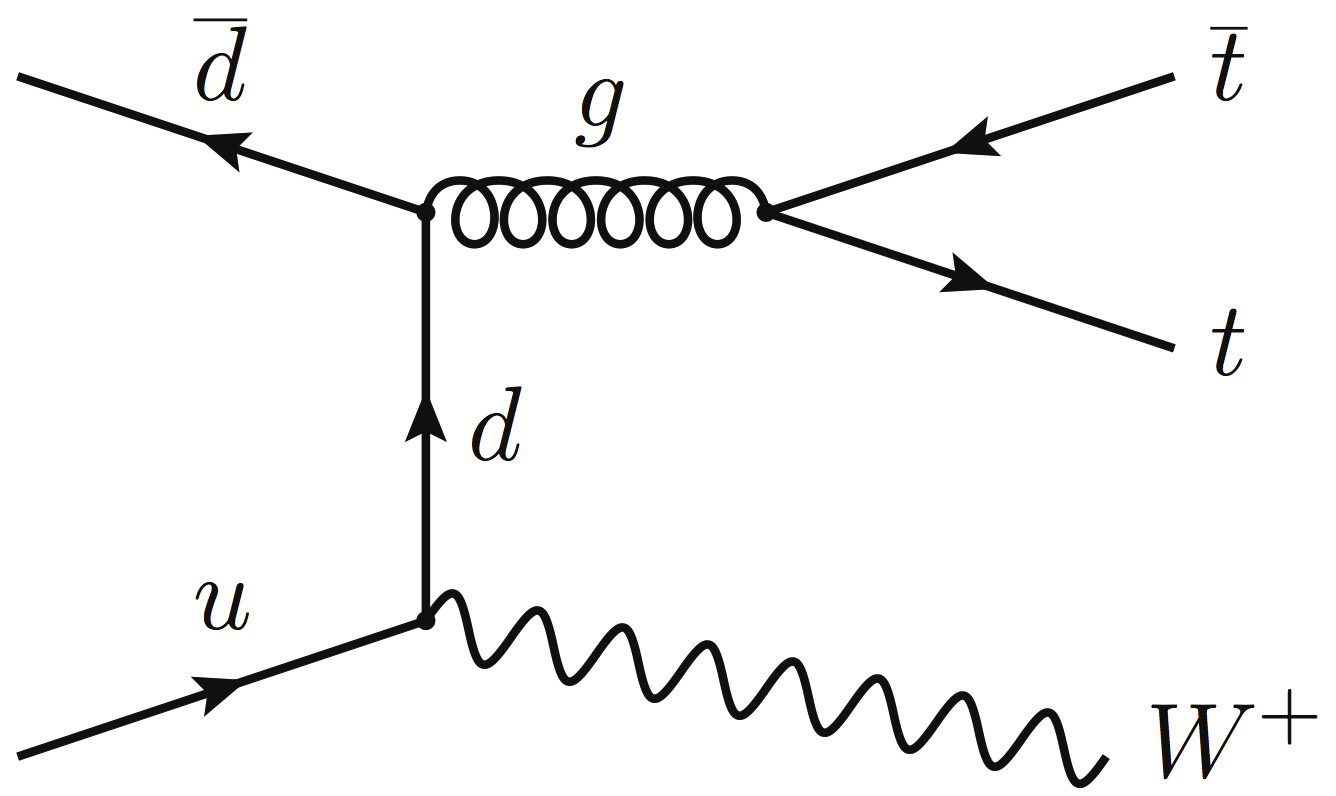
\includegraphics[width=0.35\textwidth]{Plots/ttV/ttW}
  \caption{Examples of tree-level Feynman diagrams . \label{intro:sig}}
\end{figure}

\clearpage
\section{ttbb}
\label{sec:ttbb}

\subsection{Samples}
Four Monte Carlo (MC) generators are compared in this study. % , where the inclusive $\mathrm{t\bar{t}}$ PP8 sample was previously used as the nominal background estimate in the ttH analysis. 
One sample is generated with the \textsc{POWHEG-BOX v2} NLO event generator~\cite{Nason:2004rx,Frixione:2007vw,Alioli:2010xd,Campbell:2014kua} with NNPDF3.0 NLO PDF set, matched to Pythia8 and is referred to as PP8 $\mathrm{t\bar{t}}$, where the additional bb-pair is described by the parton shower. The $h_{damp}$ parameter was set to 1.5 times the top quark mass~\cite{ATL-PHYS-PUB-2016-020}, which is assumed to be 172.5~GeV. The parton shower and the hadronisation were modelled by Pythia 8.210~\cite{PhysRevD.78.014026} with the A14 set of tuned parameters~\cite{ATL-PHYS-PUB-2014-021}. The renormalisation and factorisation scales were set to the transverse mass of the top quark, defined as $m_{T,t} = \sqrt{m^2_t + p^2_{T,t}}$, where $p_{T,t}$ is the transverse momentum of the top quark in the $t\overline{t}$ center-of-mass reference frame. This sample was previously used as the nominal background estimate in the ttH(bb) analysis.
The intrinsic uncertainty of the nominal PP8 $\mathrm{t\bar{t}}$ sample is expressed by the simultaneous variation of the renormalisation and factorisation scales ($\mu_R$ and $\mu_F$) together with the corresponding A14 Eigentune variation parameters. The RadiationUp variation has the renormalisation and factorisation scales decreased by a factor of two, the Var3c upward variation of the A14 parameter set and the $h_{damp}$ parameter doubled. The RadiationDown variation has the renormalisation and factorisation scales increased by a factor of two, the Var3c downward variation and the nominal value of $h_{damp}$.
Additionally, the up and down radiation uncertainty is calculated following the CMS approach, under which the renormalisation scale, factorisation scale and PDF tune variations are each taken individually and their difference to the nominal is summed in quadrature, without changing $h_{damp}$.

The PP8 $\mathrm{t\bar{t}b\bar{b}}$ sample uses the \textsc{POWHEG-BOX-RES} generator~\cite{jeo2015treatment} and \textsc{OPENLOOPS}~\cite{Cascioli:2011va}, where $t\bar{t}+b\bar{b}$ matrix elements are calculated at NLO with massive b-quarks, using the four-flavour NNPDF30 NLO as 0118 4FS PDF set~\cite{Jezo:2018yaf}. The parton shower and hadronisation is modelled by Pythia 8.240. The b-quark mass is set to 4.95~GeV in \textsc{POWHEG}. The scales are set to $\mu_R=\sqrt[4]{m_{T,t}\times m_{T,\bar{t}}\times m_{T,b}\times m_{T,\bar{b}} }$, $\mu_F=0.5\times(m_{T,t}+m_{T,\bar{t}}+m_{T,b}+ m_{T,\bar{b}}+m_{T,gluon})$ and $h_{damp}=H_T/2$.

For the PP8 samples the bottom and charm quark decays are described by \textsc{EVTGEN} v1.2~\cite{LANGE2001152} and the top quark spin correlations follow ref.~\cite{Frixione:2007zp}.

The \textsc{Sherpa} $\mathrm{t\bar{t}b\bar{b}}$ sample was generated using \textsc{Sherpa}-\textsc{Openloops}~\cite{Cascioli:2013era}. The $t\bar{t}b\bar{b}$ matrix elements were calculated with massive b-quarks at NLO, using the \textsc{COMIX}~\cite{gleisberg2008comix} and \textsc{OPENLOOPS}~\cite{Cascioli:2011va} matrix element generators, and merged with the Sherpa parton shower, tuned by the authors~\cite{schumann2007parton}. The four-flavour NNPDF30 NNLO as 0118 4FS PDF set was used. The q-quark mass is set to 4.75~GeV. The scales are set to $\mu_R=\sqrt[4]{m_{T,t}\times m_{T,\bar{t}}\times m_{T,b}\times m_{T,\bar{b}}}$ and $\mu_F=H_T/2$.

Both the PP8 $\mathrm{t\bar{t}b\bar{b}}$ and the \textsc{Sherpa} $\mathrm{t\bar{t}b\bar{b}}$ samples describe the additional bb-pair with NLO precision in QCD, taking into account the b-quark mass.

The \textsc{Sherpa} $\mathrm{t\bar{t}}$ sample uses \textsc{Sherpa} version 2.2.1~\cite{Gleisberg:2008ta} with the \textsc{MEPS}@NLO (multi-leg) setup using the \textsc{MEPS}@NLO prescription~\cite{Hoeche:2012yf}, interfaced with \textsc{Openloops}. It provides NLO accuracy for up to one additional parton and LO accuracy for up to four additional partons. The NNPDF3.0 NNLO PDF set is used with a five-flavour scheme and both renormalisation and factorisation scales are set to $\sqrt{0.5\times(m_{T,t}^2+m_{T,\bar{t}}^2)}$. 
A summary of all samples used is given in Table~\ref{tab:ttbbsamples}. All samples are filtered to contain only semi-leptonic $\mathrm{t\bar{t}}$ decays.

\begin{table}
\begin{center}
\caption{\label{tab:ttbbsamples}
The configurations used for the event generation of ttbb processes.}
\vspace{0.25cm}
{\small
\setlength\tabcolsep{1.5pt}
\begin{tabular}{llllll}
\hline\hline
Process & Generator & ME order & Parton shower & PDF & Tune  \\
%& (alternative) & (alternative) & & \\
\hline
$\ttbar$  & \textsc{PowHeg v2} & \textsc{NLO} & \textsc{Pythia 8} &  5FS NNPDF3.0 NLO & \textsc{A14}  \\
$\ttbar+b\bar{b}$  & \textsc{Powheg-Box-Res} & \textsc{NLO} & \textsc{Pythia 8} &  4FS NNPDF30 NLO as 0118& \textsc{A14}  \\
$\ttbar+b\bar{b}$  & \textsc{Sherpa 2.2.1} & \textsc{NLO} & \textsc{Sherpa} &  4FS NNPDF30 NNLO as 0118 & \textsc{Sherpa} default  \\
$\ttbar$  & \textsc{Sherpa 2.2.1} & tt+0,1\@NLO+2,3,4@LO & \textsc{Sherpa} &  5FS NNPDF3.0 NNLO & \textsc{Sherpa} default  \\
\hline\hline
\end{tabular}
}
\end{center}
\end{table}

\subsection{Fiducial Volume}
Object and event selection is defined at particle-level that closely matches the detector-level described in reference~\cite{HIGG-2017-03} and was defined together with CMS as a common phase space. Jets are reconstructed from stable particles with a mean lifetime of $\tau > 3\times 10^{-11}$~s, using the anti-$k_t$ algorithm with a radius parameter of $R=0.4$, are required to have transverse momentum $p_{T}>25~\GeV$ and pseudorapidity $|\eta|< 2.5$. Jets that are matched to b-hadrons with $p_{T}>5~\GeV$ by ghost matching~\cite{Cacciari:2008gn} and are referred to as b-jets. Electrons and muons, referred to as leptons, are required to satisfy $p_{T}>27~\GeV$ and $|\eta|< 2.5$. 
Leptons are removed if they are separated from a jet by less than $\Delta R=0.4$ ($\Delta R = \sqrt{(\Delta \eta )^2 + (\Delta \phi)^2}$).
%Selected leptons are required to be separated from selected jets by $\Delta R>0.4$. 
Events are selected with exactly one lepton and at least 4 jets, equivalent to the semi-leptonic $\mathrm{t\bar{t}}$ decay.
%Two regions are considered, defined by 3 b-jets or $\geq$4 b-jets.
Two analysis regions are considered. The first is defined by the presence of exactly three selected $b$-jets (3b selection), while the second requires four or more such $b$-jets (4b selection).


%, , , , , , $N_{jets}$, 
\begin{table}[]
\begin{center}
\caption{\label{tab:ttbb_varlist}
The list of the validation variables for the comparison of the generators for $ttbb$ process.}
\vspace{0.25cm}
{\small
\setlength\tabcolsep{1.5pt}
\begin{tabular}{l|l}
\hline\hline
Variable & Description  \\ \hline
average $\Delta R (b,b)$&    average over $\Delta R(b, b)$ build from all 2 b-jet combinations in the event           \\ 
min $\Delta R (b,b)$ &    $\Delta R$ of the two b-jets in the event which are closest in $\Delta R $          \\ 
$M (b,b)_{maxP_T}$ &      mass of the 2 b-jet system build of the b-jets with maximal $p_T$         \\ 
$M (b,b)_{min\Delta R(b,b)}$ &         mass of the 2 b-jet system build of the b-jets closest in $\Delta R $     \\ 
$H_T$  $b$-jets&           scalar sum of all b-jet $p_T$ in the event    \\ 
$H_T$ light-jets&        scalar sum of $p_T$ of all light jets in the event       \\ 
$N_{jets}$   &     number of all jets in the event (including b-jets)          \\ 
jet eta &          $\eta$ of any jet in the event     \\ 
    \hline\hline    
\end{tabular}
}
\end{center}
\end{table}




\subsection{Results}
The nominal PP8 $\mathrm{t\bar{t}}$ sample and the alternative generators are normalised to an integral of 1, after all cuts and in each histogram individually for a shape-only comparison.
The radiation uncertainty variations on PP8 $\mathrm{t\bar{t}}$ are added and include normalisation differences with respect to the central value. For the RadiationUp uncertainty, an alternative sample with different $h_{damp}$ was used, here the number of events (not the sum of weights) was scaled to the central value.
The central value of the PP8 $\mathrm{t\bar{t}}$ and the other three generators are normalised to 1. The first ratio plot shows the ratio of the different MC samples to PP8 $\mathrm{t\bar{t}}$ from the upper plot, where the colour scheme is given in the legend.
The list of the validation variables for this comparison is presented in this note summarised in Table~\ref{tab:ttbb_varlist}.

Discrepancies between PP8 $\mathrm{t\bar{t}}$ and the alternative generators can be seen in the $\Delta R$ quantities, as in Figures~\ref{ttbb:avedR} and \ref{ttbb:mindR}, where at least in the 4b selection the difference to the alternative generators is larger than the uncertainty band given by the radiation variations.  
%In the b-jet pair invariant mass variables $\mathrm{M_{bb}^{max P_T}}$ and $\mathrm{M_{bb}^{min \Delta R}}$ shown in Figures~\ref{ttbb:MbbmaxPT} and~\ref{ttbb:MbbminDR}, the largest difference is seen between the Sherpa $\mathrm{t\bar{t}}$ and all other samples.
Two types of $b$-jet pairs are defined: one pair is build from the two $b$-jets with the highest $p_T$ sum, called $maxP_T$, and one pair from the two $b$-jets which are closest in $\Delta R$, called $min \Delta R$ . The invariant mass of the b-jet pairs are shown in Figures~\ref{ttbb:MbbmaxPT} and~\ref{ttbb:MbbminDR}, the largest difference is seen between the Sherpa $\mathrm{t\bar{t}}$ and all other samples.
%
Differences are also observed in the $\mathrm{H_T}$ distributions, particularly in the 3b selection. In $\mathrm{H_T}$ of all b-jets, as in Figures~\ref{ttbb:HTbjets}, one observes a difference between PP8 $\mathrm{t\bar{t}}$ and the samples with b-jets in the matrix element, while in $\mathrm{H_T}$ of all light jets, shown in Figure~\ref{ttbb:HTljets}, a difference between the 4 and 5 flavour schemes can be seen. The jet multiplicity, as in Figure~\ref{ttbb:Njets}, has poor agreement among the generators for large jet multiplicities.
Lastly, differences among the samples are shown for the $\mathrm{\eta_{jet}}$ distribution, in Figure~\ref{ttbb:jeteta}.

The second ratio plot shows the relative uncertainty of the radiation variations on PP8 $\mathrm{t\bar{t}}$, shown as the ratio of the varied sample to the nominal for two cases described above, where the scale and A14 Eigentune parameters are either varied simultaneously (black) or individually and then summed following the CMS approach (red). $h_{damp}$ variations are only considered for the first case.



\begin{figure}[!htb]
\centering
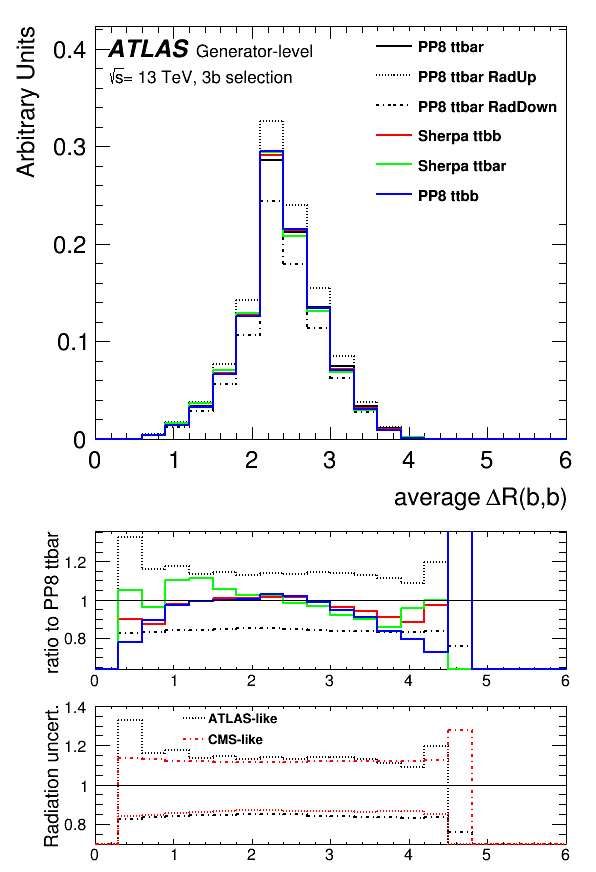
\includegraphics[width=0.38\textwidth]{Plots/ttbb/hisgenEvt_Dr_GenBJetsAverage_4j3t__div}
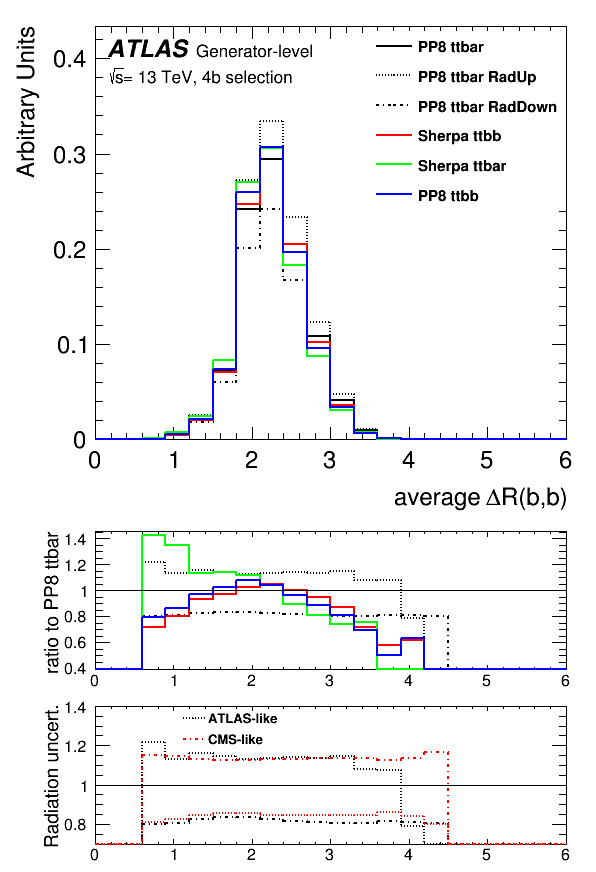
\includegraphics[width=0.38\textwidth]{Plots/ttbb/hisgenEvt_Dr_GenBJetsAverage_4j4t__div}
  \caption{Distribution of the average opening angle between two b-jets, for the 3b selection (left) and the 4b-jet selection (right). The central value of the PP8 $\mathrm{t\bar{t}}$ and the other three generators are normalised to 1. The first ratio shows the different curves divided by PP8 $\mathrm{t\bar{t}}$. The second ratio plot shows the relative uncertainty of the radiation variations divided by the nominal PP8 $\mathrm{t\bar{t}}$ following the above description of simultaneous variations (black) and as the sum of individual variations following the CMS approach (red).  \label{ttbb:avedR}}
\end{figure}

\begin{figure}[!htb]
\centering
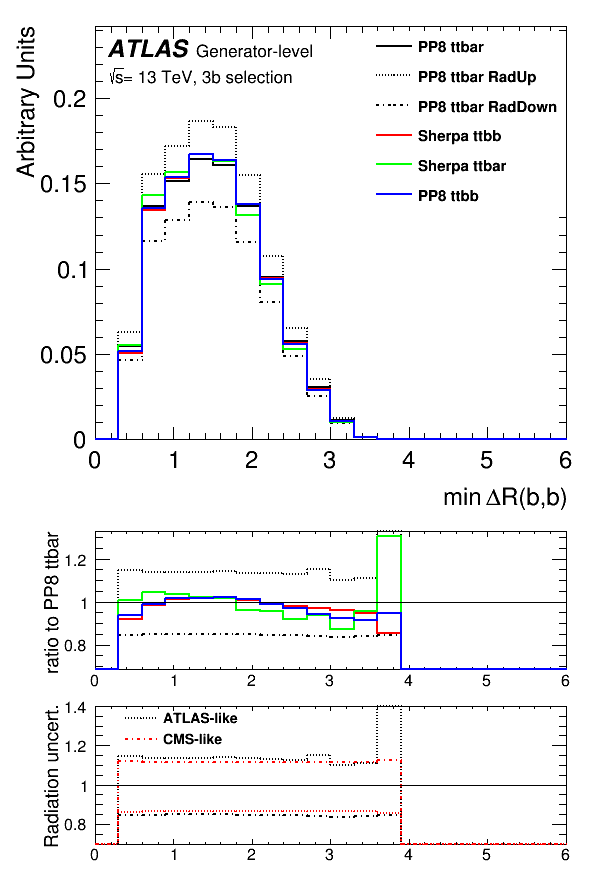
\includegraphics[width=0.38\textwidth]{Plots/ttbb/hisgenEvt_Dr_MinDeltaRGenBJets_4j3t__div}
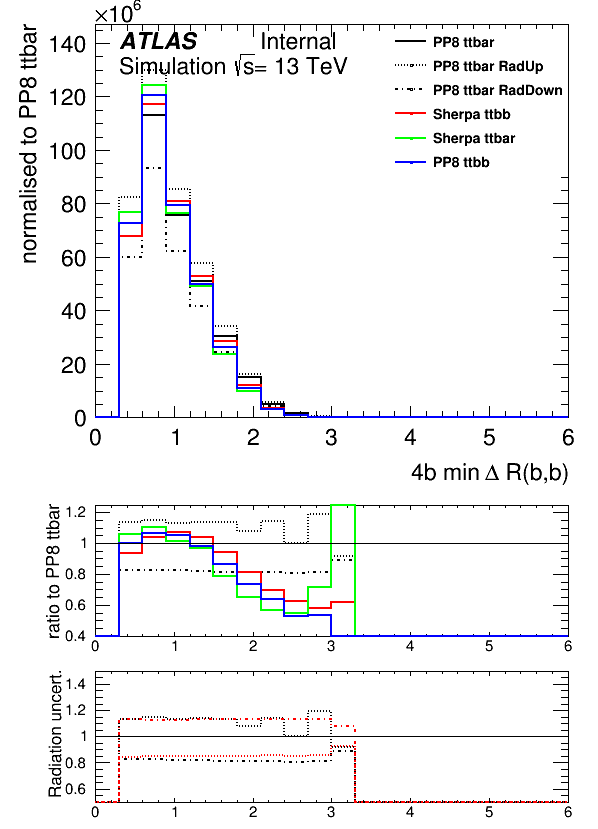
\includegraphics[width=0.38\textwidth]{Plots/ttbb/hisgenEvt_Dr_MinDeltaRGenBJets_4j4t__div}
  \caption{Distribution of the smallest opening angle between two b-jets, for the 3b selection (left) and the 4b-jet selection (right). The central value of the PP8 $\mathrm{t\bar{t}}$ and the other three generators are normalised to 1. The first ratio shows the different curves divided by PP8 $\mathrm{t\bar{t}}$. The second ratio plot shows the relative uncertainty of the radiation variations divided by the nominal PP8 $\mathrm{t\bar{t}}$ following the above description of simultaneous variations (black) and as the sum of individual variations following the CMS approach (red). \label{ttbb:mindR}}
\end{figure}

\begin{figure}[!htb]
\centering
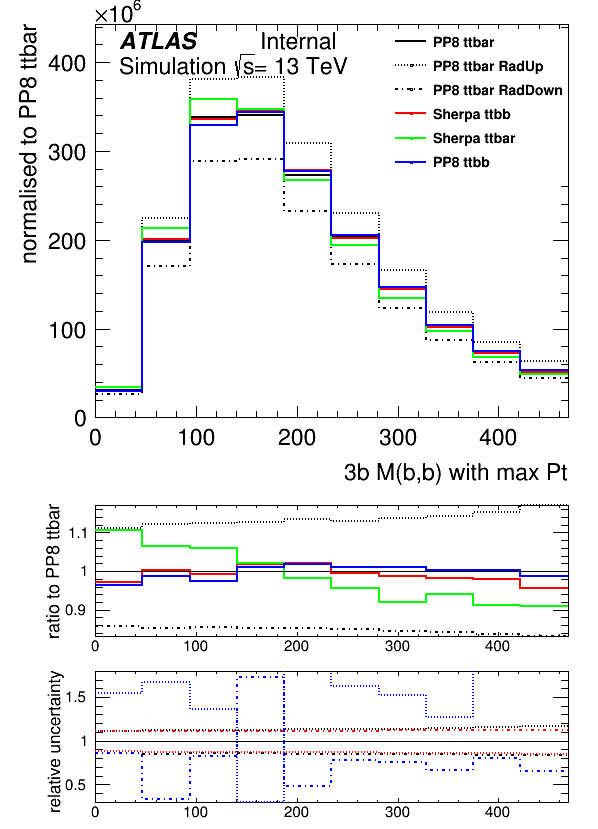
\includegraphics[width=0.38\textwidth]{Plots/ttbb/hisgenEvt_M_HardestGenBJets_4j3t__div}
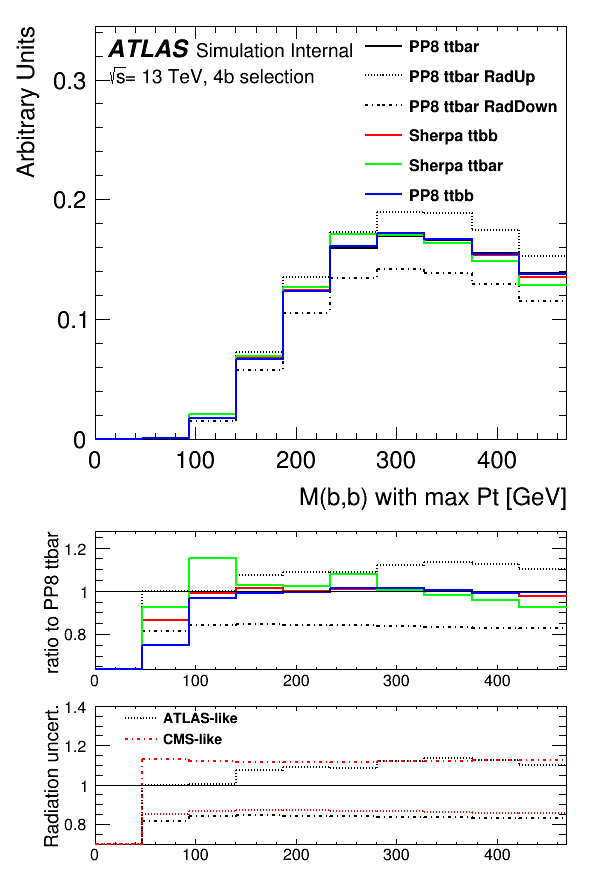
\includegraphics[width=0.38\textwidth]{Plots/ttbb/hisgenEvt_M_HardestGenBJets_4j4t__div}
  \caption{Distribution of the invariant mass in GeV of the two b-jets with the highest $\mathrm{P_T}$ sum, for the 3b selection (left) and the 4b-jet selection (right). The central value of the PP8 $\mathrm{t\bar{t}}$ and the other three generators are normalised to 1. The first ratio shows the different curves divided by PP8 $\mathrm{t\bar{t}}$. The second ratio plot shows the relative uncertainty of the radiation variations divided by the nominal PP8 $\mathrm{t\bar{t}}$ following the above description of simultaneous variations (black) and as the sum of individual variations following the CMS approach (red). \label{ttbb:MbbmaxPT}}
\end{figure}

\begin{figure}[!htb]
\centering
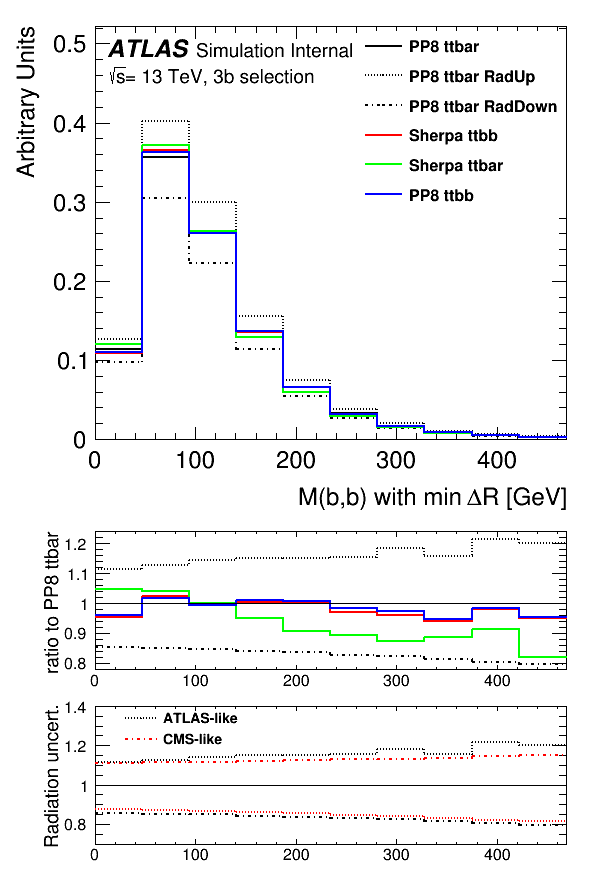
\includegraphics[width=0.38\textwidth]{Plots/ttbb/hisgenEvt_M_MinDeltaRGenBJets_4j3t__div}
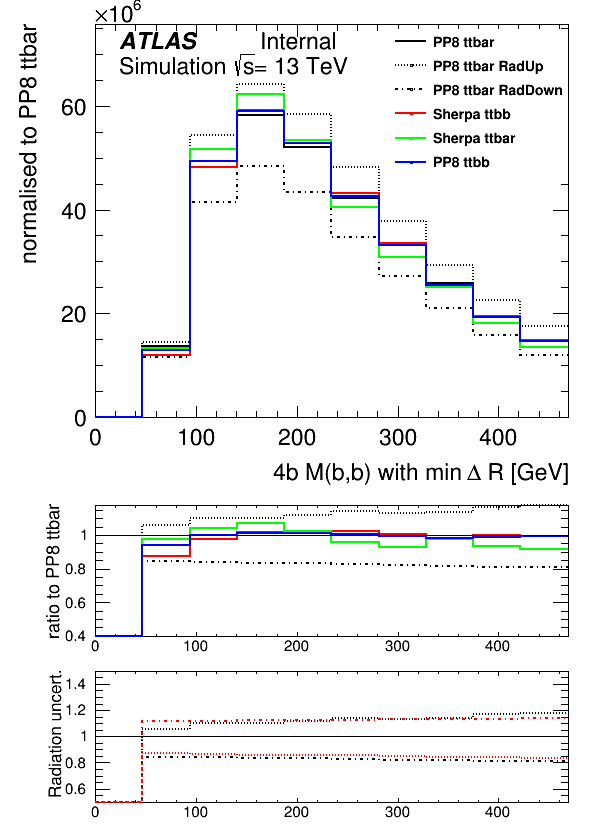
\includegraphics[width=0.38\textwidth]{Plots/ttbb/hisgenEvt_M_MinDeltaRGenBJets_4j4t__div}
  \caption{Distribution of the invariant mass in GeV of the two b-jets with the smallest opening angle, for the 3b selection (left) and the 4b-jet selection (right). The central value of the PP8 $\mathrm{t\bar{t}}$ and the other three generators are normalised to 1. The first ratio shows the different curves divided by PP8 $\mathrm{t\bar{t}}$. The second ratio plot shows the relative uncertainty of the radiation variations divided by the nominal PP8 $\mathrm{t\bar{t}}$ following the above description of simultaneous variations (black) and as the sum of individual variations following the CMS approach (red). \label{ttbb:MbbminDR}}
\end{figure}

\begin{figure}[!htb]
\centering
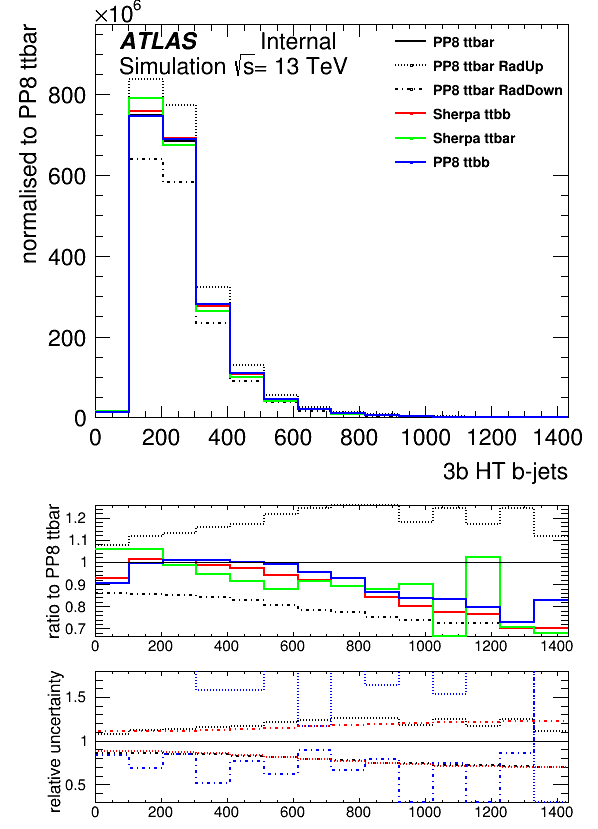
\includegraphics[width=0.38\textwidth]{Plots/ttbb/hisgenHTbjets_4j3t__div}
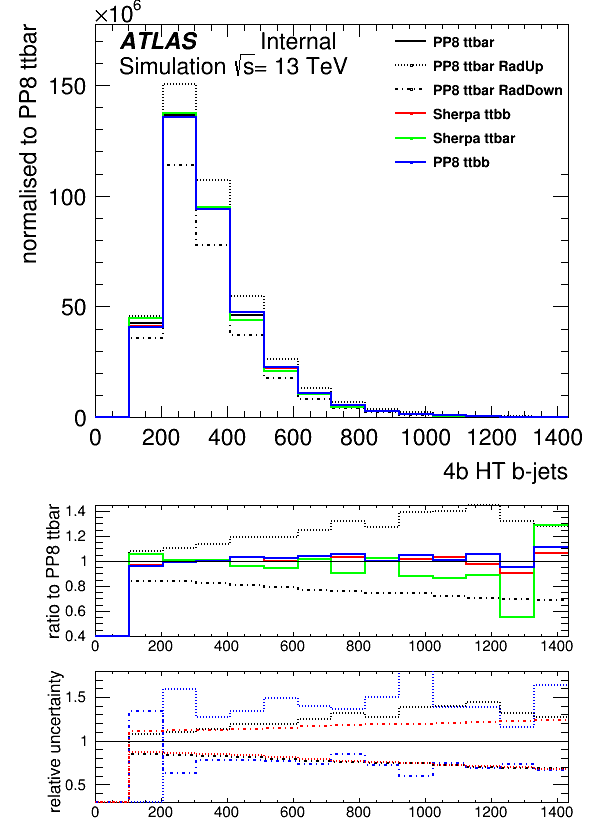
\includegraphics[width=0.38\textwidth]{Plots/ttbb/hisgenHTbjets_4j4t__div}
  \caption{Sum of b-jet transverse momenta in GeV, for the 3b selection (left) and the 4b-jet selection (right). The central value of the PP8 $\mathrm{t\bar{t}}$ and the other three generators are normalised to 1. The first ratio shows the different curves divided by PP8 $\mathrm{t\bar{t}}$. The second ratio plot shows the relative uncertainty of the radiation variations divided by the nominal PP8 $\mathrm{t\bar{t}}$ following the above description of simultaneous variations (black) and as the sum of individual variations following the CMS approach (red). \label{ttbb:HTbjets}}
\end{figure}

\begin{figure}[!htb]
\centering
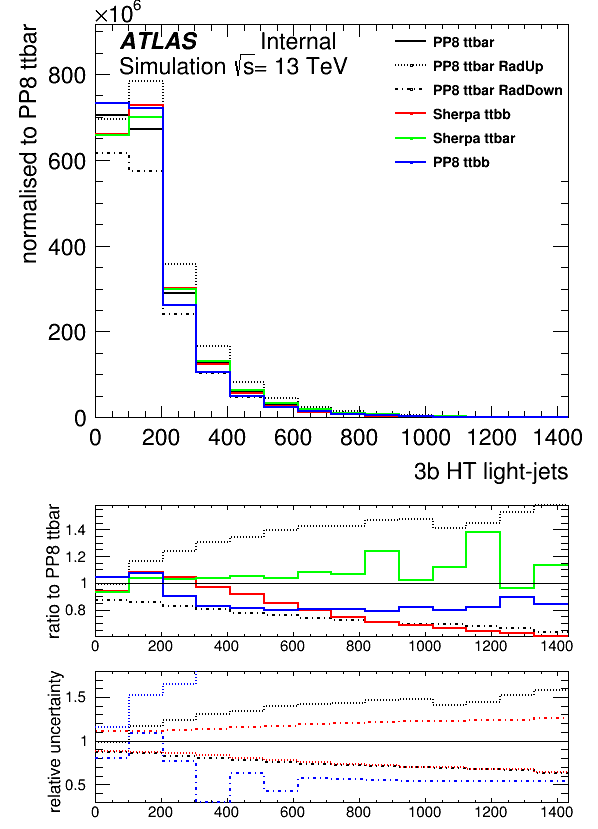
\includegraphics[width=0.38\textwidth]{Plots/ttbb/hisgenHTljets_4j3t__div}
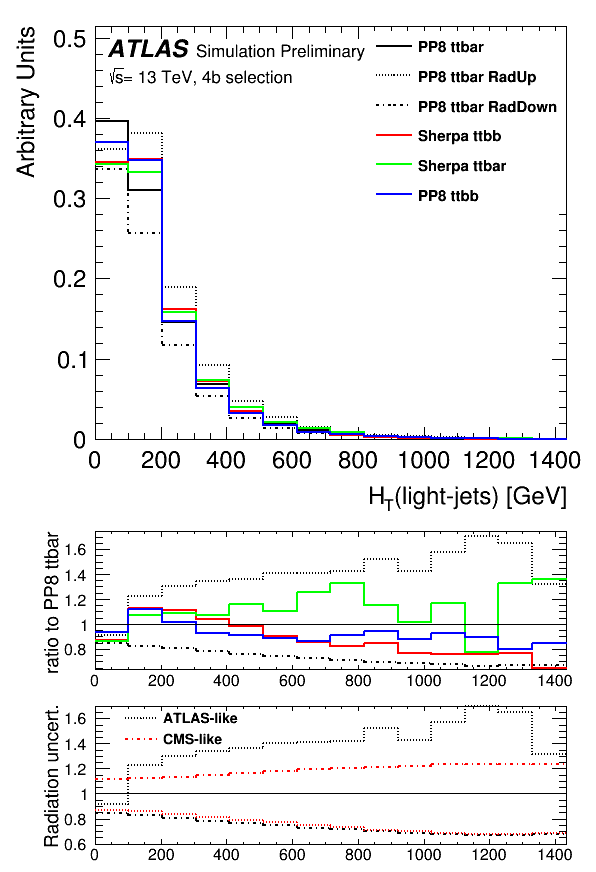
\includegraphics[width=0.38\textwidth]{Plots/ttbb/hisgenHTljets_4j4t__div}
  \caption{Sum of non-b-jet transverse momenta in GeV, for the 3b selection (left) and the 4b-jet selection (right). The central value of the PP8 $\mathrm{t\bar{t}}$ and the other three generators are normalised to 1. The first ratio shows the different curves divided by PP8 $\mathrm{t\bar{t}}$. The second ratio plot shows the relative uncertainty of the radiation variations divided by the nominal PP8 $\mathrm{t\bar{t}}$ following the above description of simultaneous variations (black) and as the sum of individual variations following the CMS approach (red). \label{ttbb:HTljets}}
\end{figure}

\begin{figure}[!htb]
\centering
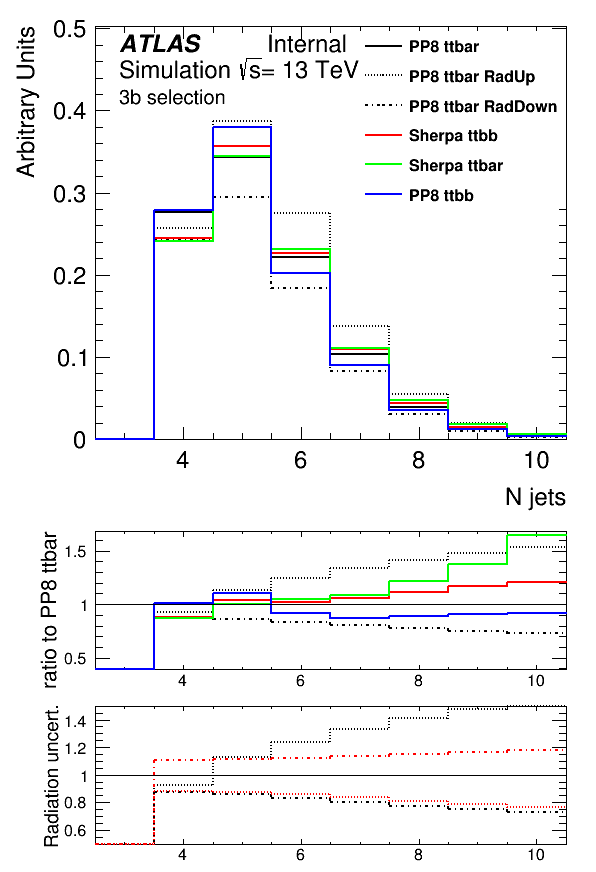
\includegraphics[width=0.38\textwidth]{Plots/ttbb/hisgenNjets_4j3t__div}
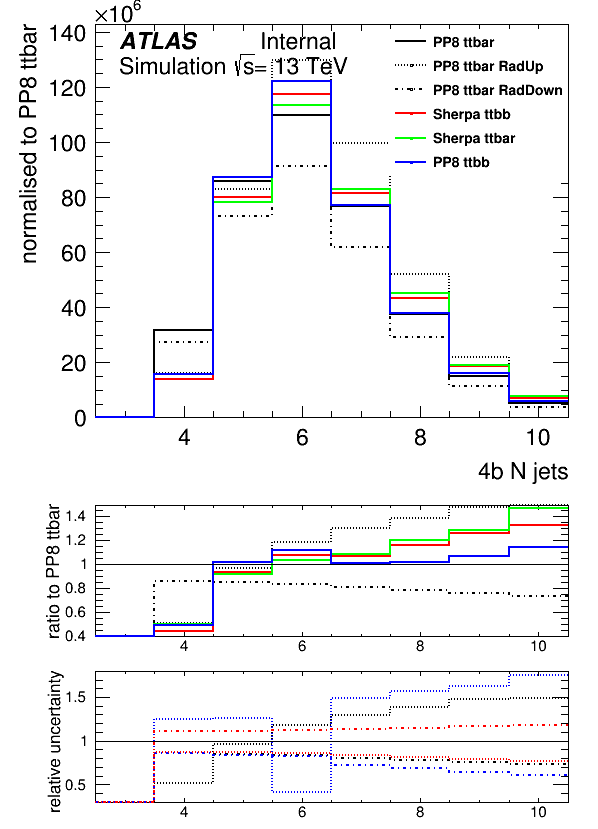
\includegraphics[width=0.38\textwidth]{Plots/ttbb/hisgenNjets_4j4t__div}
  \caption{Jet multiplicity, for the 3b selection (left) and the 4b-jet selection (right). The central value of the PP8 $\mathrm{t\bar{t}}$ and the other three generators are normalised to 1. The first ratio shows the different curves divided by PP8 $\mathrm{t\bar{t}}$. The second ratio plot shows the relative uncertainty of the radiation variations divided by the nominal PP8 $\mathrm{t\bar{t}}$ following the above description of simultaneous variations (black) and as the sum of individual variations following the CMS approach (red). \label{ttbb:Njets}}
\end{figure}

\begin{figure}[!htb]
\centering
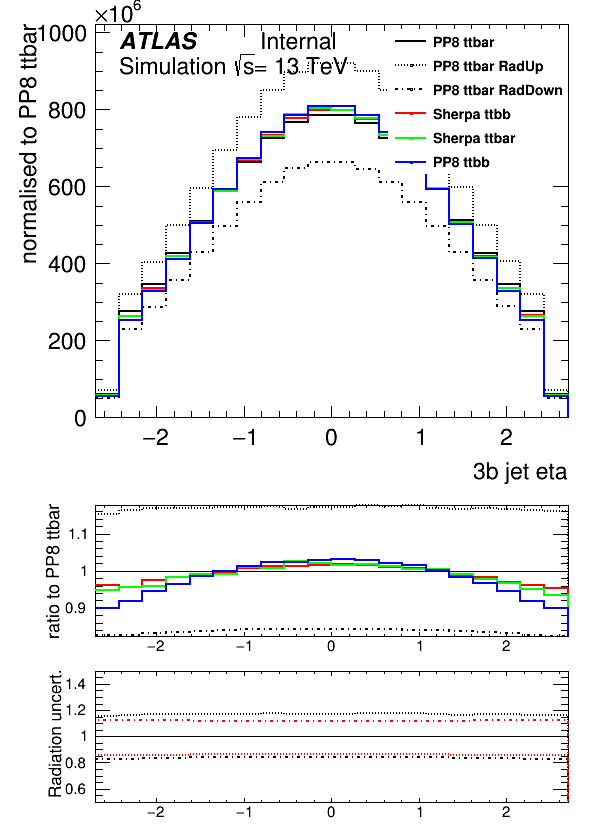
\includegraphics[width=0.38\textwidth]{Plots/ttbb/his3b_jeteta__div}
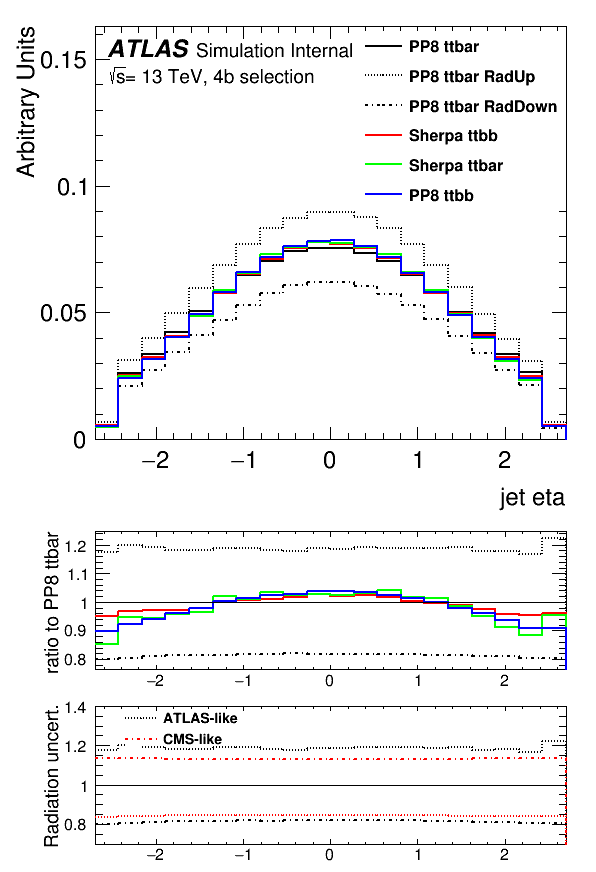
\includegraphics[width=0.38\textwidth]{Plots/ttbb/his4b_jeteta__div}
  \caption{Jet pseudorapidity, for the 3b selection (left) and the 4b-jet selection (right). The central value of the PP8 $\mathrm{t\bar{t}}$ and the other three generators are normalised to 1. The first ratio shows the different curves divided by PP8 $\mathrm{t\bar{t}}$. The second ratio plot shows the relative uncertainty of the radiation variations divided by the nominal PP8 $\mathrm{t\bar{t}}$ following the above description of simultaneous variations (black) and as the sum of individual variations following the CMS approach (red). \label{ttbb:jeteta}}
\end{figure}
\clearpage
\section{$t\bar{t}W$ process}
\label{sec:ttV}


\subsection{Samples}
Two MC generators are compared in this study.
The nominal sample for \ttW production was generated using the \textsc{Sherpa}~2.2.1~\cite{sherpa} generator with the NNPDF3.0 NLO PDF set.
The matrix element (ME) was calculated for up to one additional parton at NLO and up to two partons at LO using
\textsc{Comix}~\cite{Gleisberg:2008fv} and \textsc{OpenLoops}~\cite{Cascioli:2011va}, and merged with the \textsc{Sherpa} parton shower~\cite{Schumann:2007mg} using the \textsc{MePs@Nlo} prescription~\cite{Hoeche:2012yf}.
The choice of renormalisation and factorisation scales is $\mu_R = \mu_F = H_\textrm{T}$/2, where $H_\textrm{T}$ is defined as the scalar sum of the transverse masses $\sqrt{p_\textrm{T}^2+m^2}$ of all final state particles.



Systematic uncertainties due to missing higher-order QCD corrections are estimated by varying the factorisation and renormalisation scales in the nominal sample simultaneously by a factor of 0.5 and 2.0 with respect to the central value. 
Uncertainties associated with the modelling of additional QCD radiation are estimated by comparing the nominal \ttW prediction with that of an alternative sample that was generated at NLO with the \textsc{MadGraph5\_aMC@NLO}~2.2.1 generator using the same scale choice and PDF set as for the nominal sample, and interfaced to \textsc{Pythia}~8.2 in combination with the A14 tune. 
The samples configurations are summarised in Table~\ref{tab:mcconfig}.
%%%%%%%%%%%%%%%%%%%%%%%%%%%%%%%%%%%%%%%%
\begin{table}
\begin{center}
\caption{\label{tab:mcconfig}
The configurations used for the event generation of \ttW processes.}
\vspace{0.25cm}
{\small
\setlength\tabcolsep{1.5pt}
\begin{tabular}{llllll}
\hline\hline
Process & Generator & ME order & Parton shower & PDF & Tune  \\
%& (alternative) & (alternative) & & \\
\hline
$\ttbar W$  & \textsc{Sherpa 2.2.1} & \textsc{MePs@Nlo} & \textsc{Sherpa} &  NNPDF3.0 NNLO & \textsc{Sherpa} default \\
& \textsc{MG5\_aMC} & NLO & \textsc{Pythia} 8 & NNPDF3.0 NLO & A14   \\
\hline\hline
\end{tabular}
}
\end{center}
\end{table}


% Finally, the uncertainty due to the choice of PDF set is evaluated using the PDF4LHC15 prescription.

\subsection{Fiducial Volume}
\label{sec:ttw_fid}
Object and event selection is defined at particle-level that closely matches the detector-level described in reference~\cite{ATLAS-CONF-2019-045} and was defined together with CMS as a common phase space. 
Jets are reconstructed from stable particles with a mean lifetime of $\tau > 3\times 10^{-11}$~s, using the anti-$k_t$ algorithm with a radius parameter of $R=0.4$.
Jets are required to satisfy $\pt > 25~\gev$ and $|\eta| < 2.5$.
Jets are matched to $b$-hadrons with $\mathrm{p_{T}>5 GeV}$ by ghost matching~\cite{Cacciari:2008gn} and are referred to as $b$-jets. 
Electrons and muons, referred to as light leptons, are required to be separated from selected jets by $\Delta R>0.4$ and are otherwise removed. 
Hadronically decaying $\tau$ leptons are required to satisfy $\pt > 25~\gev$ and $|\eta| < 2.5$.
Events are selected with exactly two light leptons.
Leptons are required to have $|\eta|< 2.5$ and $\mathrm{p_{T}>25(20) GeV}$ for leading (subleading) lepton. 
Leptons are required to have same charge, targeting the semi-leptonic $\mathrm{t\bar{t}}$ decay and leptonic $W$ decay.

%Events separated by Hadronic tau decays Hadronically decaying $\tau$ lepton
Events with at least 3 jets and at least one of them being a $b$-jet are considered in the fiducial volume. 
%Events with at least 3 jets and least one $b$-jet are considered in the fiducial volume. 
The acceptance for events passing this selection is $A_X^{\geq1b\geq3j}=1.82\times10^{-2}$ for \textsc{Sherpa} and 1.90$\times10^{-2}$ for \textsc{MadGraph5\_aMC@NLO} correspondingly.
We then split into five regions, categorized by the number of jets of any flavour (three or  $\geq$4), $b$-jets (one or $\geq$2) as well as the presence of hadronically decaying $\tau$ lepton. 
				\begin{description}
				\item Region 1: 1 $N_{b-jets}$, ~ $\geq$4 $N_{jets}$ , 0-$\tau_{had}$
				\item Region 2: $\geq$2 $N_{b-jets}$,   $\geq$4 $N_{jets}$, 0-$\tau_{had}$
				\item Region 3: 1 $N_{b-jets}$, ~  3 $N_{jets}$ , 0-$\tau_{had}$
				\item Region 4: $\geq$2 $N_{b-jets}$, 3 $N_{jets}$, 0-$\tau_{had}$
				\item Region 5: $\geq$1 $N_{b-jets}$, $\geq$3 $N_{jets}$, 1-$\tau_{had}$
				\end{description}
Definitions of the regions are motivated by $t\bar{t}H$ analysis strategy.
Regions 1 and 2 corresponds to the signal regions\footnote{slightly different then in ~\cite{ATLAS-CONF-2019-045}, in order to define a common selection with the CMS collaboration} and Regions 3 and 4 are used as control regions in the 2$\ell$ same-sign  0-$\tau_{had}$ $t\bar{t}H$ channel.
Definition of Region 5 is closely followed\footnote{requirement on jet multiplicity is relaxed} by the selections in 2$\ell$ same-sign 1-$\tau_{had}$ $t\bar{t}H$ channel.

%The event selection requirements are summarized in Table~\ref{}.
%defined by 5 jets \& 3 b-jets or >=6jets \& >=4 b-jets.




\subsection{Results}
%$N_{jets}$, $N_{b-jets}$,  $HT^{\text{jets}}$, leading $b$-jet $p_T$ Leading lepton $p_T$, $|\Delta \phi _{\ell \ell }|$, $\Delta R _{\ell \ell }$, $max |\eta _l|$
\begin{table}[]
\begin{center}
\caption{\label{tab:ttw_varlist}
The list of the validation variables for the comparison of the \ttW generators.}
\vspace{0.25cm}
{\small
\setlength\tabcolsep{1.5pt}
\begin{tabular}{l|l|c}
\hline\hline
Variable & Description & Regions \\ \hline
$N_{jets}$   &     Jet multiplicity        &      1,2,5   \\ %\hline
 $N_{b-jets}$       &     Number of  $b$-jets       &   1,2,5      \\ %\hline
$HT^{\text{jets}}$      &   Sum of jets transverse momentum         &  1,2,3,4       \\ %\hline
$p_T^{b0}$       &      Leading $b$-jet transverse momentum       &   1,2      \\ %\hline
 $p_T^{\ell 0}$      &   Leading lepton transverse momentum           &     1,2,5    \\ %\hline
$\Delta R _{ \ell 0-jet }$      &     Minimum angular separation between the leading lepton and the nearest jet         &  1,2       \\ %\hline
$\Delta R _{\ell \ell }$      &       Angular distance between the two leptons      &    1,2,5    \\ %\hline
$max |\eta _l|$      &      Maximum of lepton's pseudorapidity       &     1,2    \\ %\hline
    $|\Delta \phi _{\ell \ell }|$    &    Azimuthal separation between the leptons         & 1,2    \\
    \hline\hline    
\end{tabular}
}
\end{center}
\end{table}

%Distribution of the angular distance between the two leptons (top), maximum between lepton $|\eta_{\ell 0}|$ and $|\eta_{\ell 1}|$ (centre), azimuthal separation between the leptons $\Delta \phi _{\ell \ell }$ (bottom) , for the Region 1 with 1$b$-jet (left) and Region 2 with 2$b$-jets (right) selection requiring four and more jets. 

The nominal  \textsc{Sherpa} \ttW  sample is compared to its radiation uncertainty variations and the alternative generator.
The ratio plot shows the ratio of the alternative MC sample and scale variation to the nominal sample.

The list of the validation variables for the comparison of the \ttW generators presented in this note summarised in Table~\ref{tab:ttw_varlist}.
Two sets of distribution are presented: the first comparing the shapes of the different generators - distributions are normalised to the integral, the second - comparing overall generator agreement - distributions are scaled to the generator cross section (taken directly from generation - i.e. not including any correction factors).

\subsubsection{Shape comparison}
\label{sec:ttw_shape}
In the following shape agreement between nominal and alternative generators will be presented - distributions are normalised to the integral.

Sizeable discrepancies in the modelling of jet kinematics can be seen between the \textsc{Sherpa} \ttW and \textsc{MadGraph5\_aMC@NLO} generators in 1$b$-jet selections, while in $\geq2b$-jets the difference is reduced, as illustrated in Figures~\ref{ttV:4j12b} and~\ref{ttV:3j12b} for the high (Regions 1 and 2) and low (Regions 3 and 4) jet multiplicities correspondingly. 
Differences in distributions of $b$-jet kinematics are following a similar trend - sizeable discrepancies in 1$b$-jet selections and agreed within scale uncertainties for 2$b$-jets selections, as presented on Figures~\ref{ttV:4jbinfo} for Regions 1 and 2.


\begin{figure}[!htb]
\centering
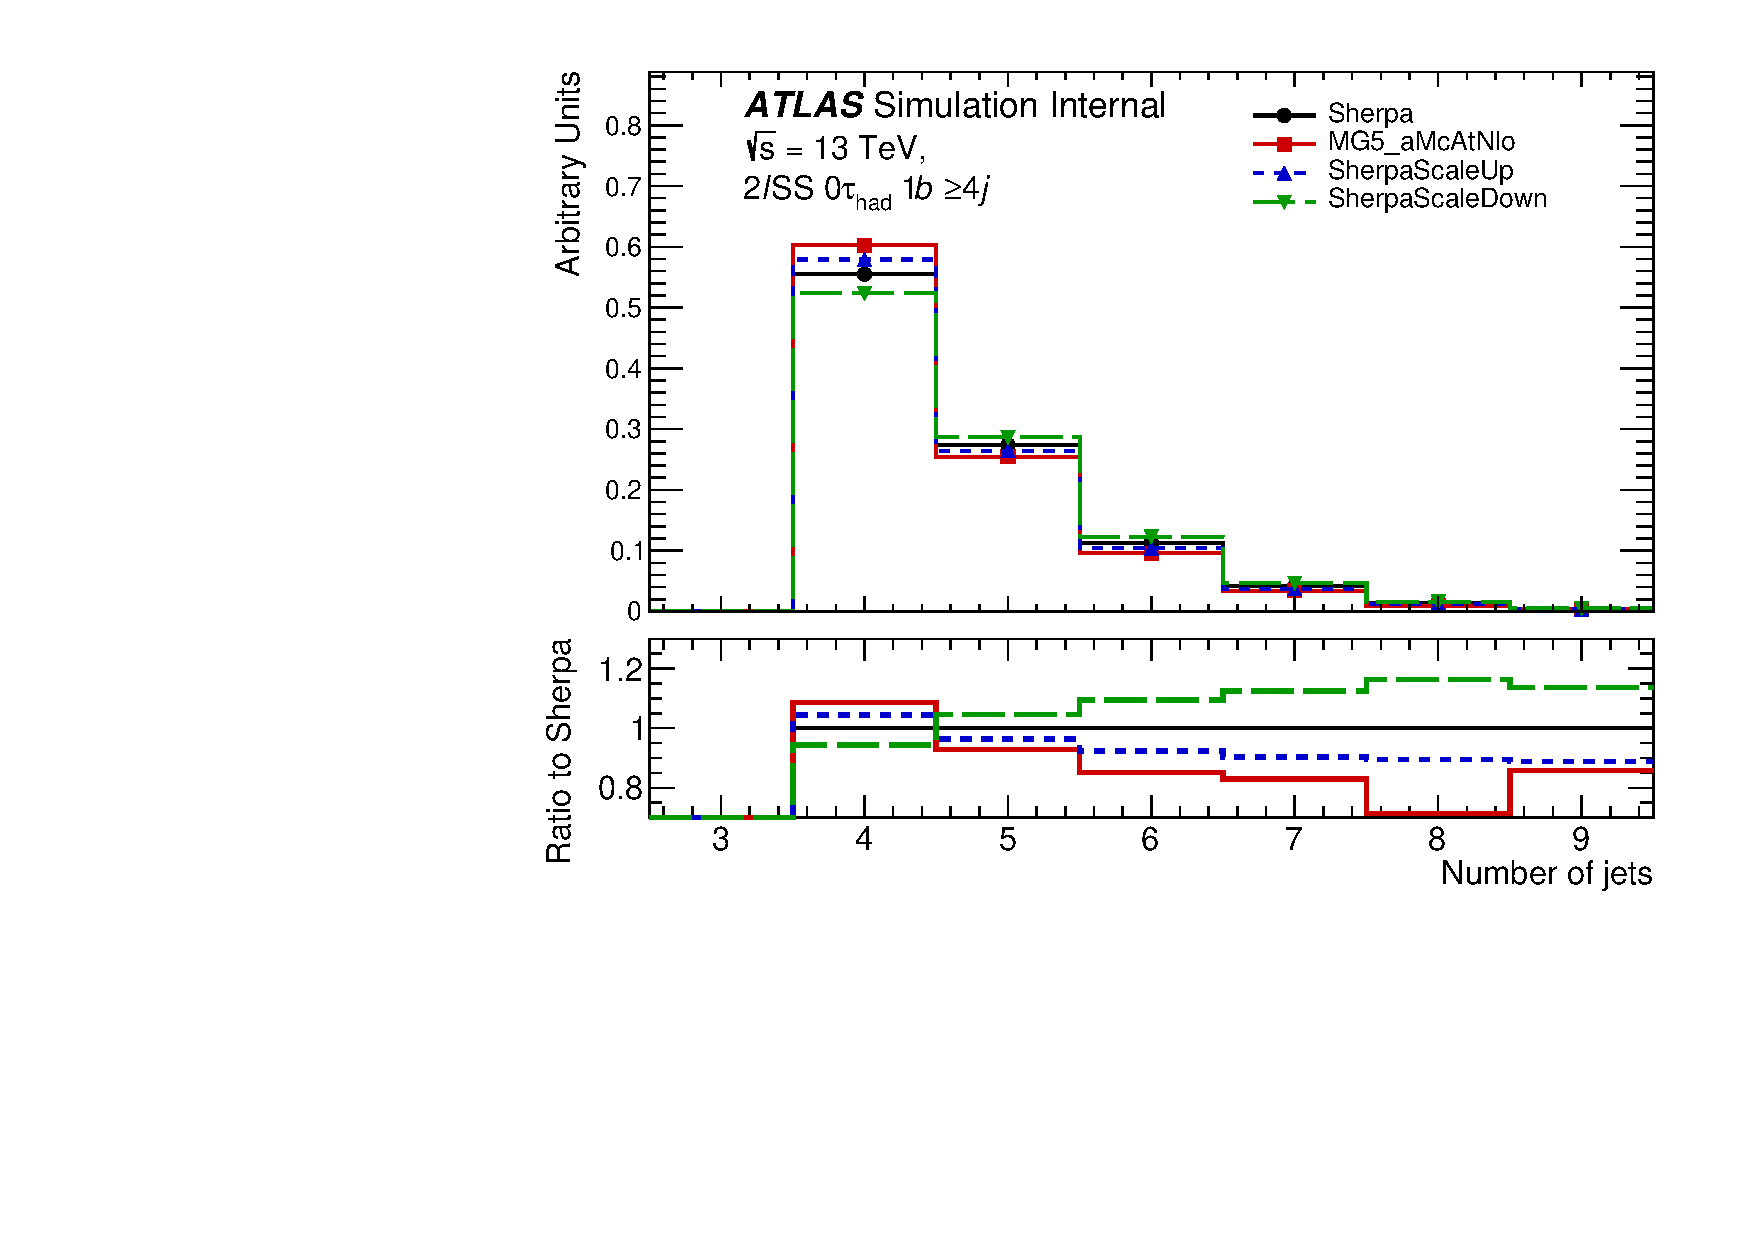
\includegraphics[width=0.45\textwidth]{Plots/ttV/shape/c_Region_0_nJets}
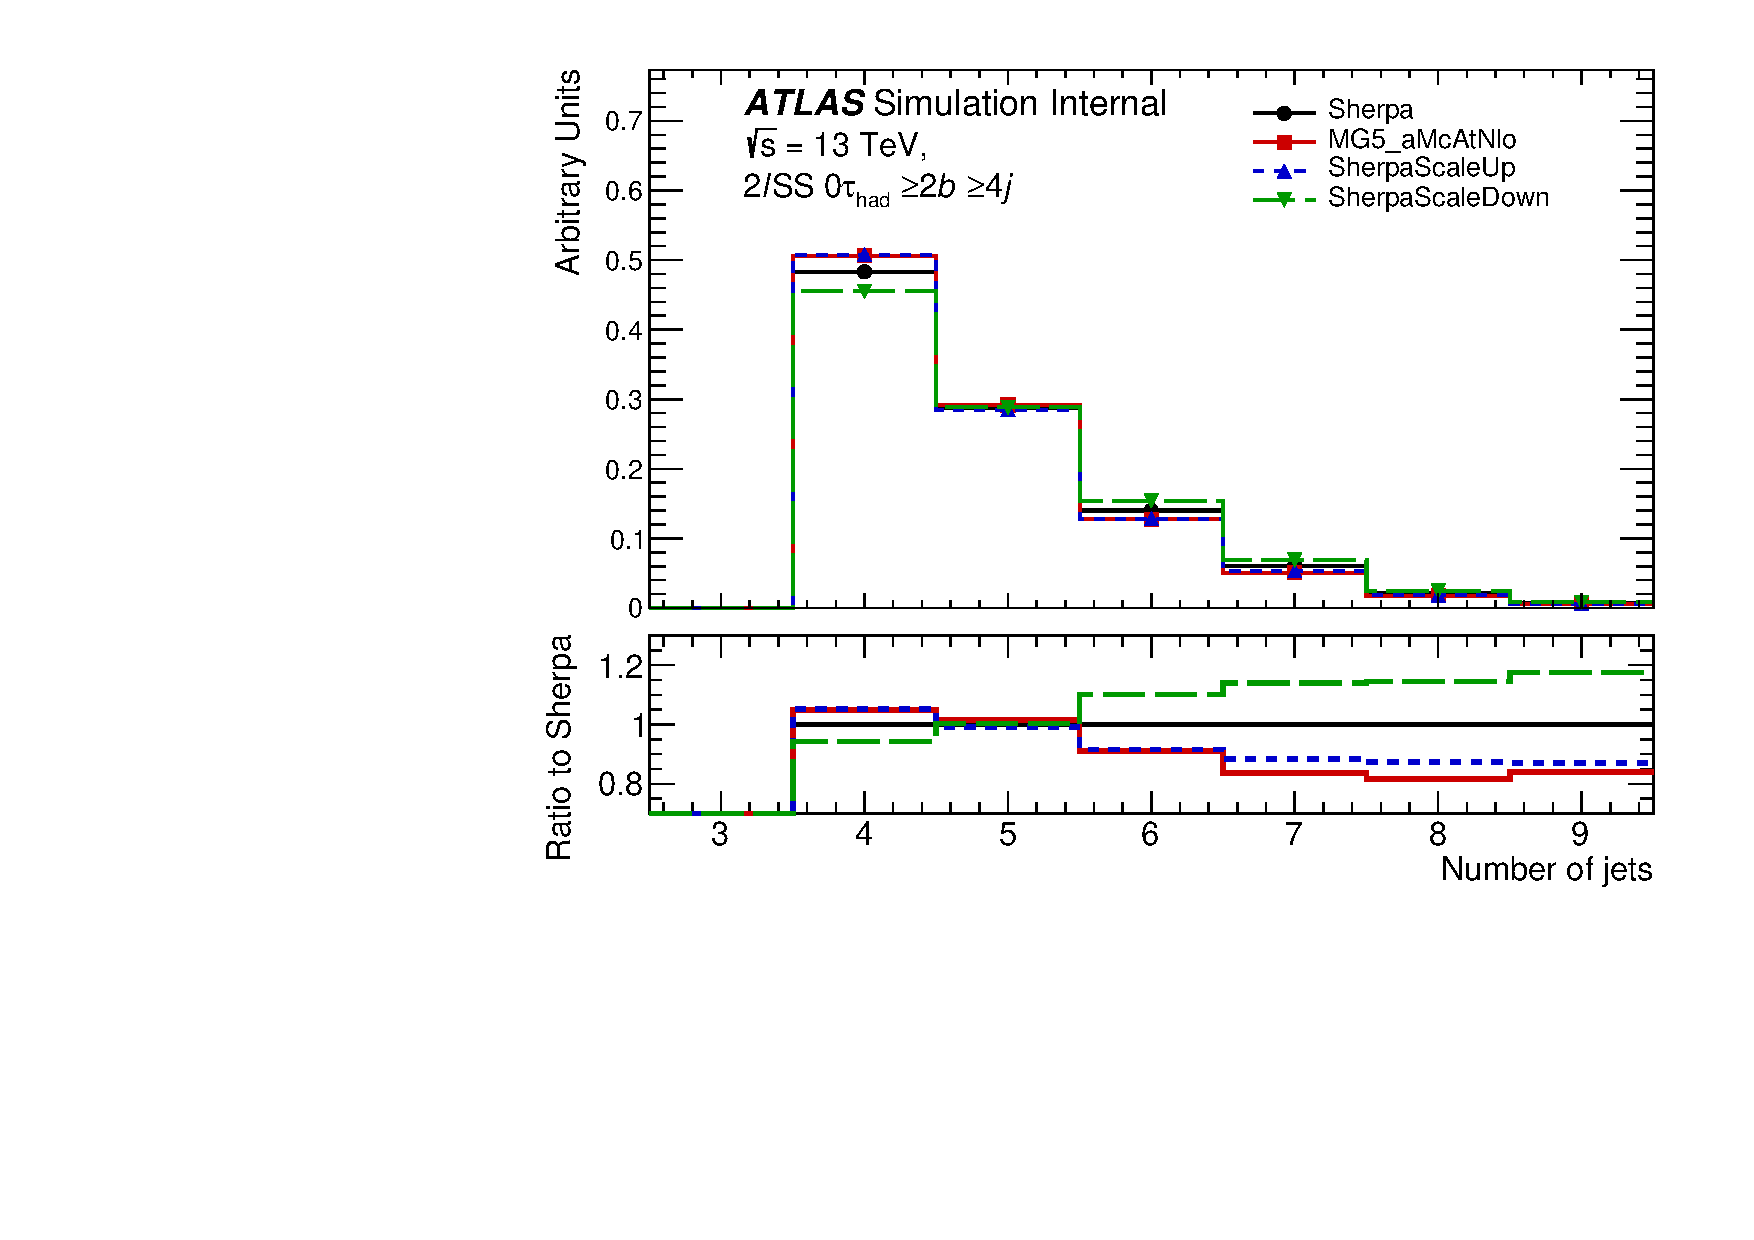
\includegraphics[width=0.45\textwidth]{Plots/ttV/shape/c_Region_1_nJets}\\
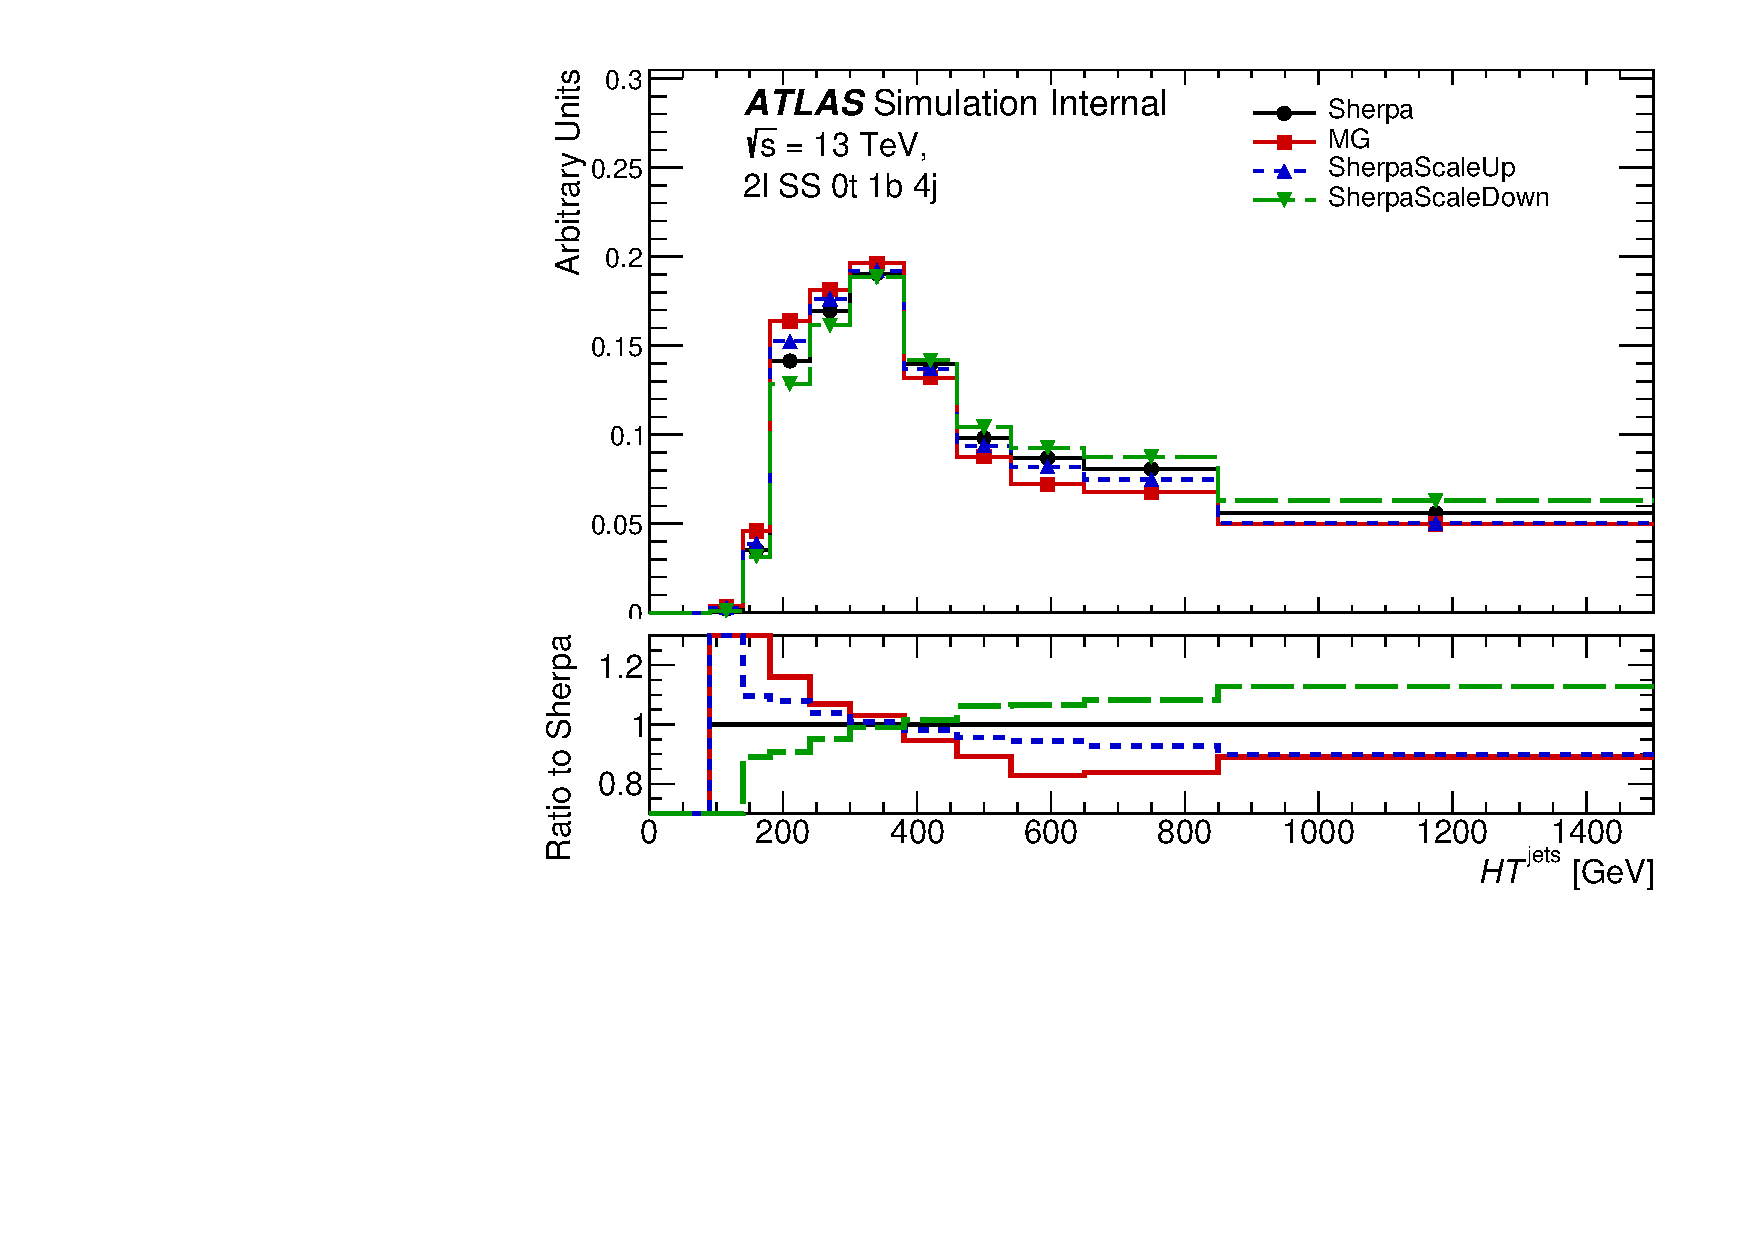
\includegraphics[width=0.45\textwidth]{Plots/ttV/shape/c_Region_0_HT_jets}
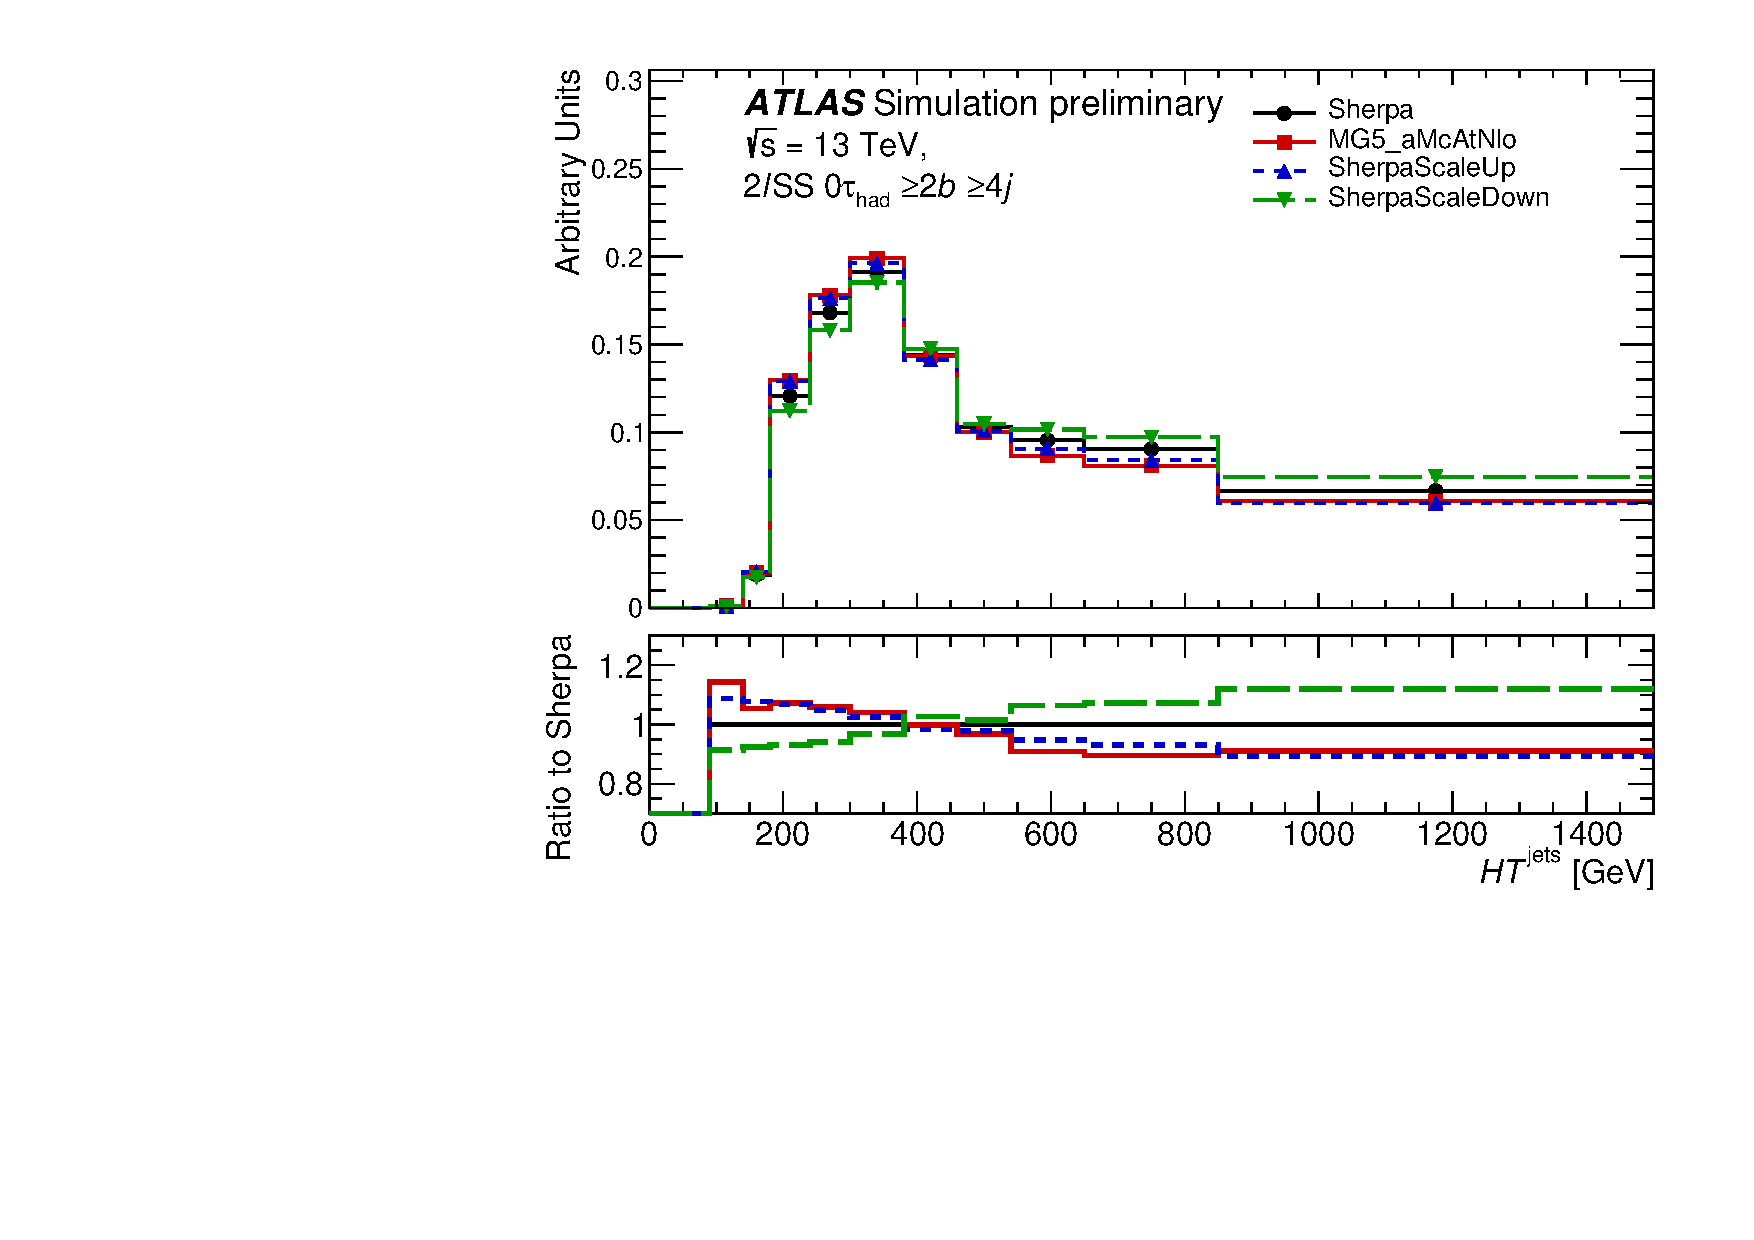
\includegraphics[width=0.45\textwidth]{Plots/ttV/shape/c_Region_1_HT_jets}\\
  \caption{Distribution of the jet multiplicities (top) and the sum of jets transverse momentum, $HT^{\text{jets}}$ (bottom), for the Region 1 with 1$b$-jet (left) and Region 2 with 2$b$-jets (right) selection requiring four and more jets. Explanation in text. \label{ttV:4j12b}}
\end{figure}


\begin{figure}[!htb]
\centering
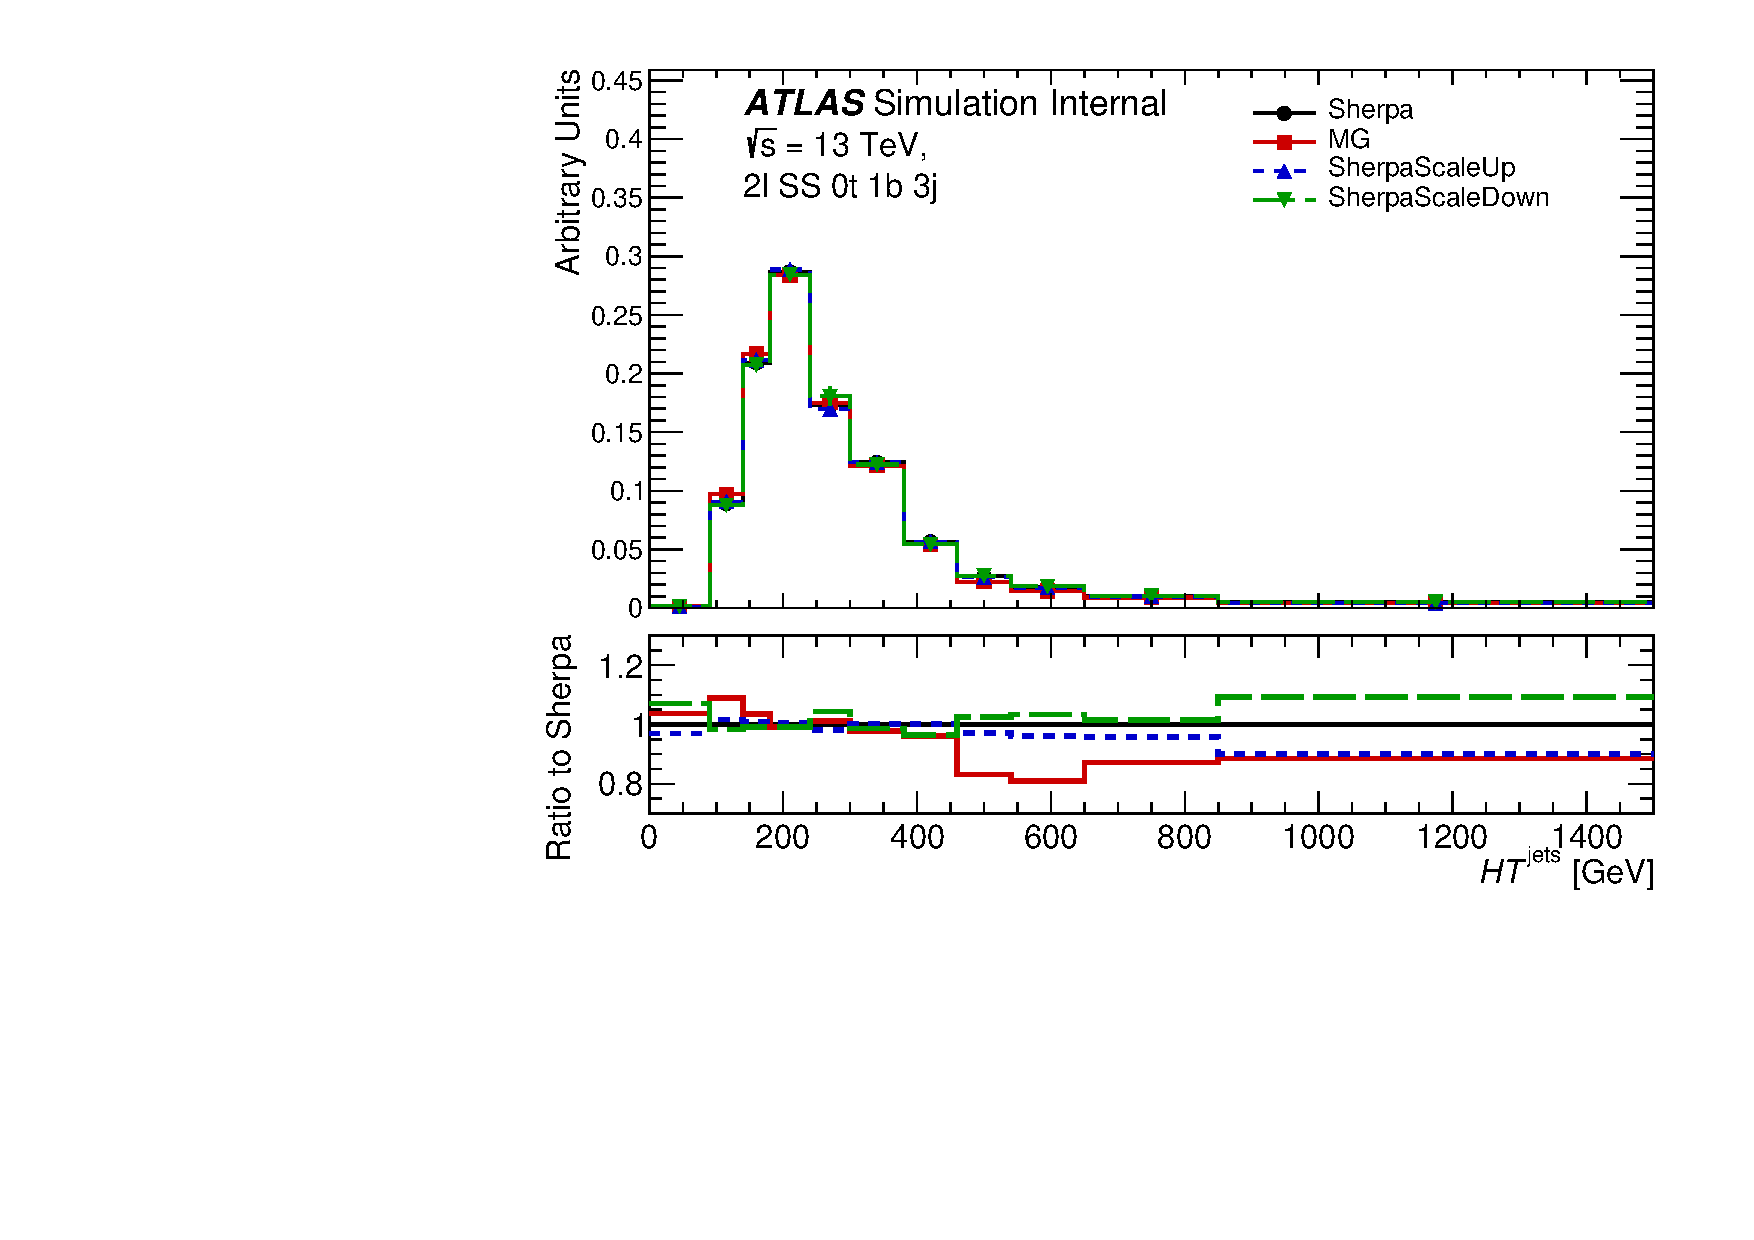
\includegraphics[width=0.45\textwidth]{Plots/ttV/shape/c_Region_2_HT_jets}
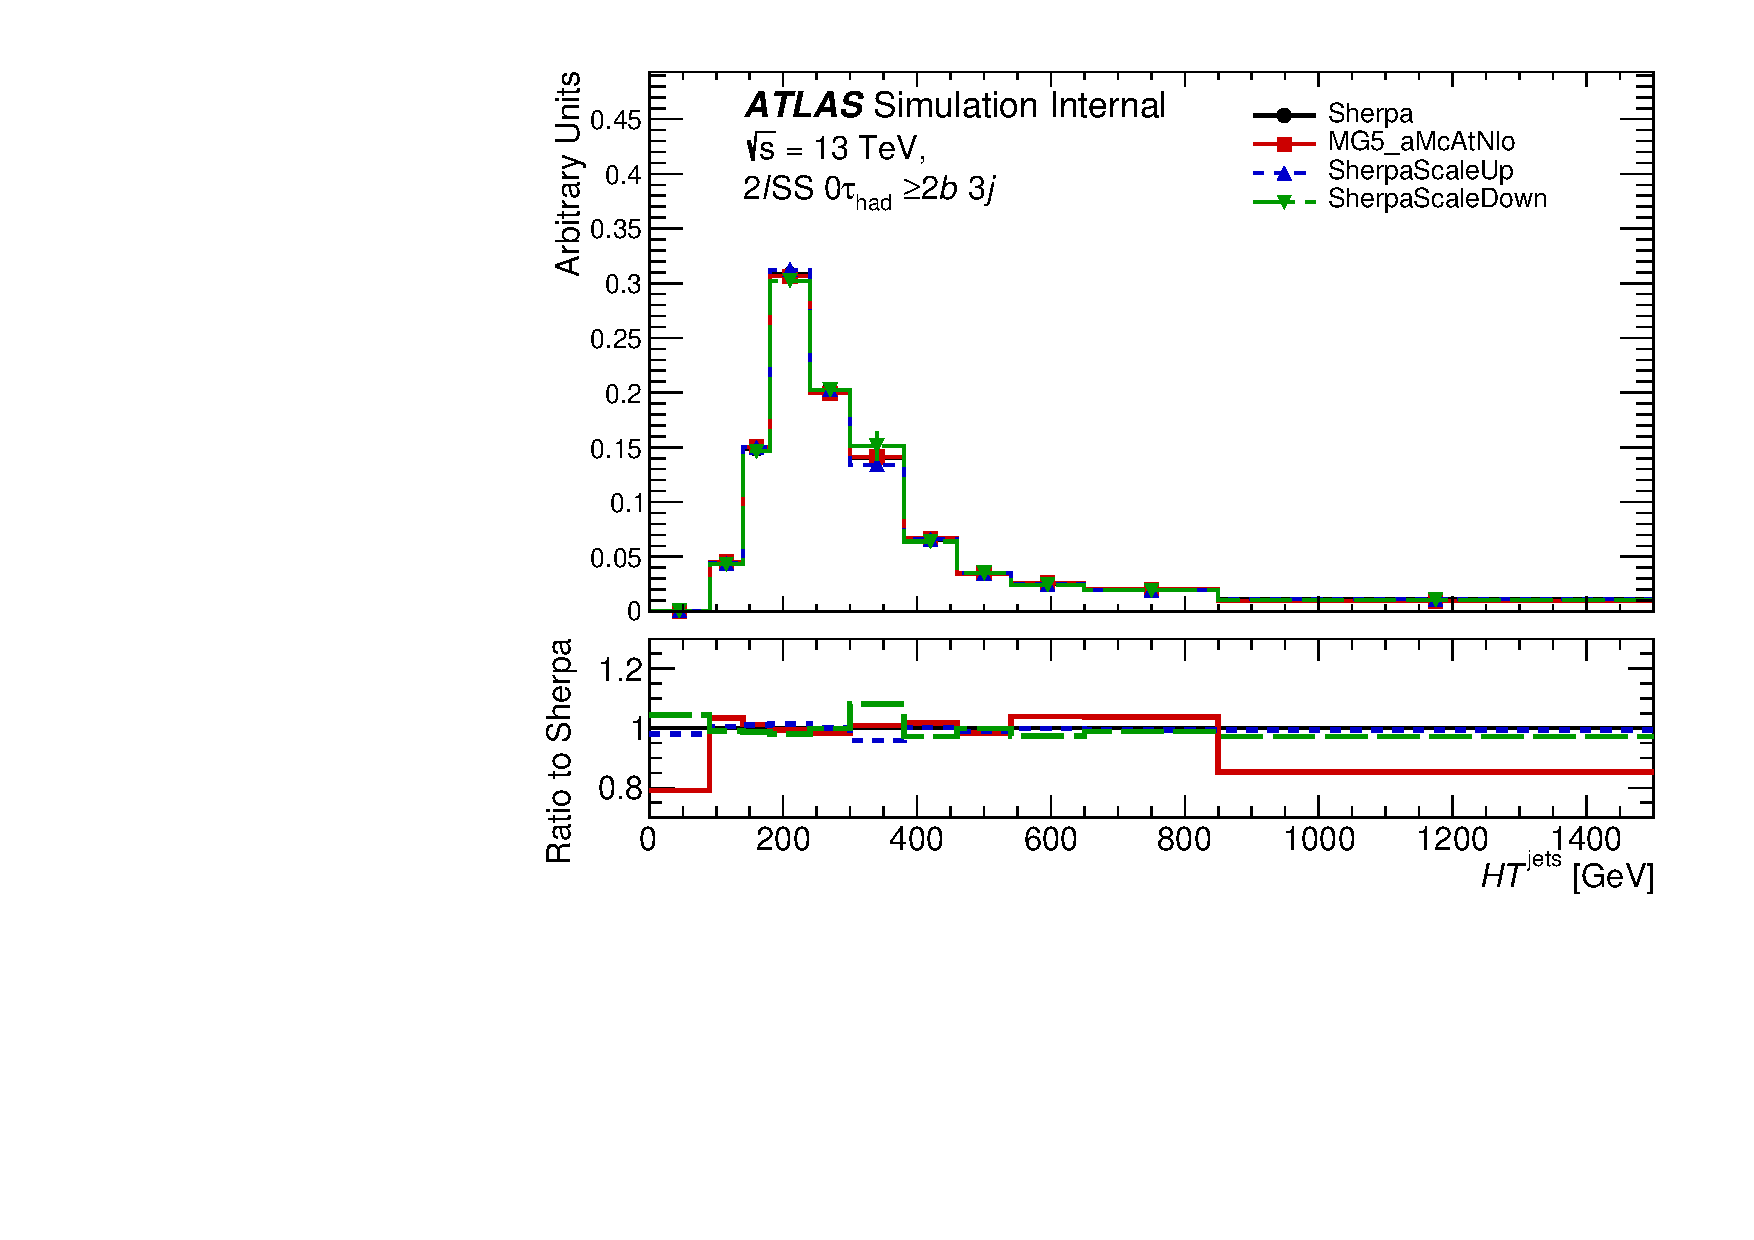
\includegraphics[width=0.45\textwidth]{Plots/ttV/shape/c_Region_3_HT_jets}\\
  \caption{Distribution of the sum of jets transverse momentum, $HT^{\text{jets}}$, for the Region 3 with 1$b$-jet (left) and Region 4 with 2$b$-jets (right) selection requiring exactly three jets. Explanation in text. \label{ttV:3j12b}}
\end{figure}


\begin{figure}[!htb]
\centering
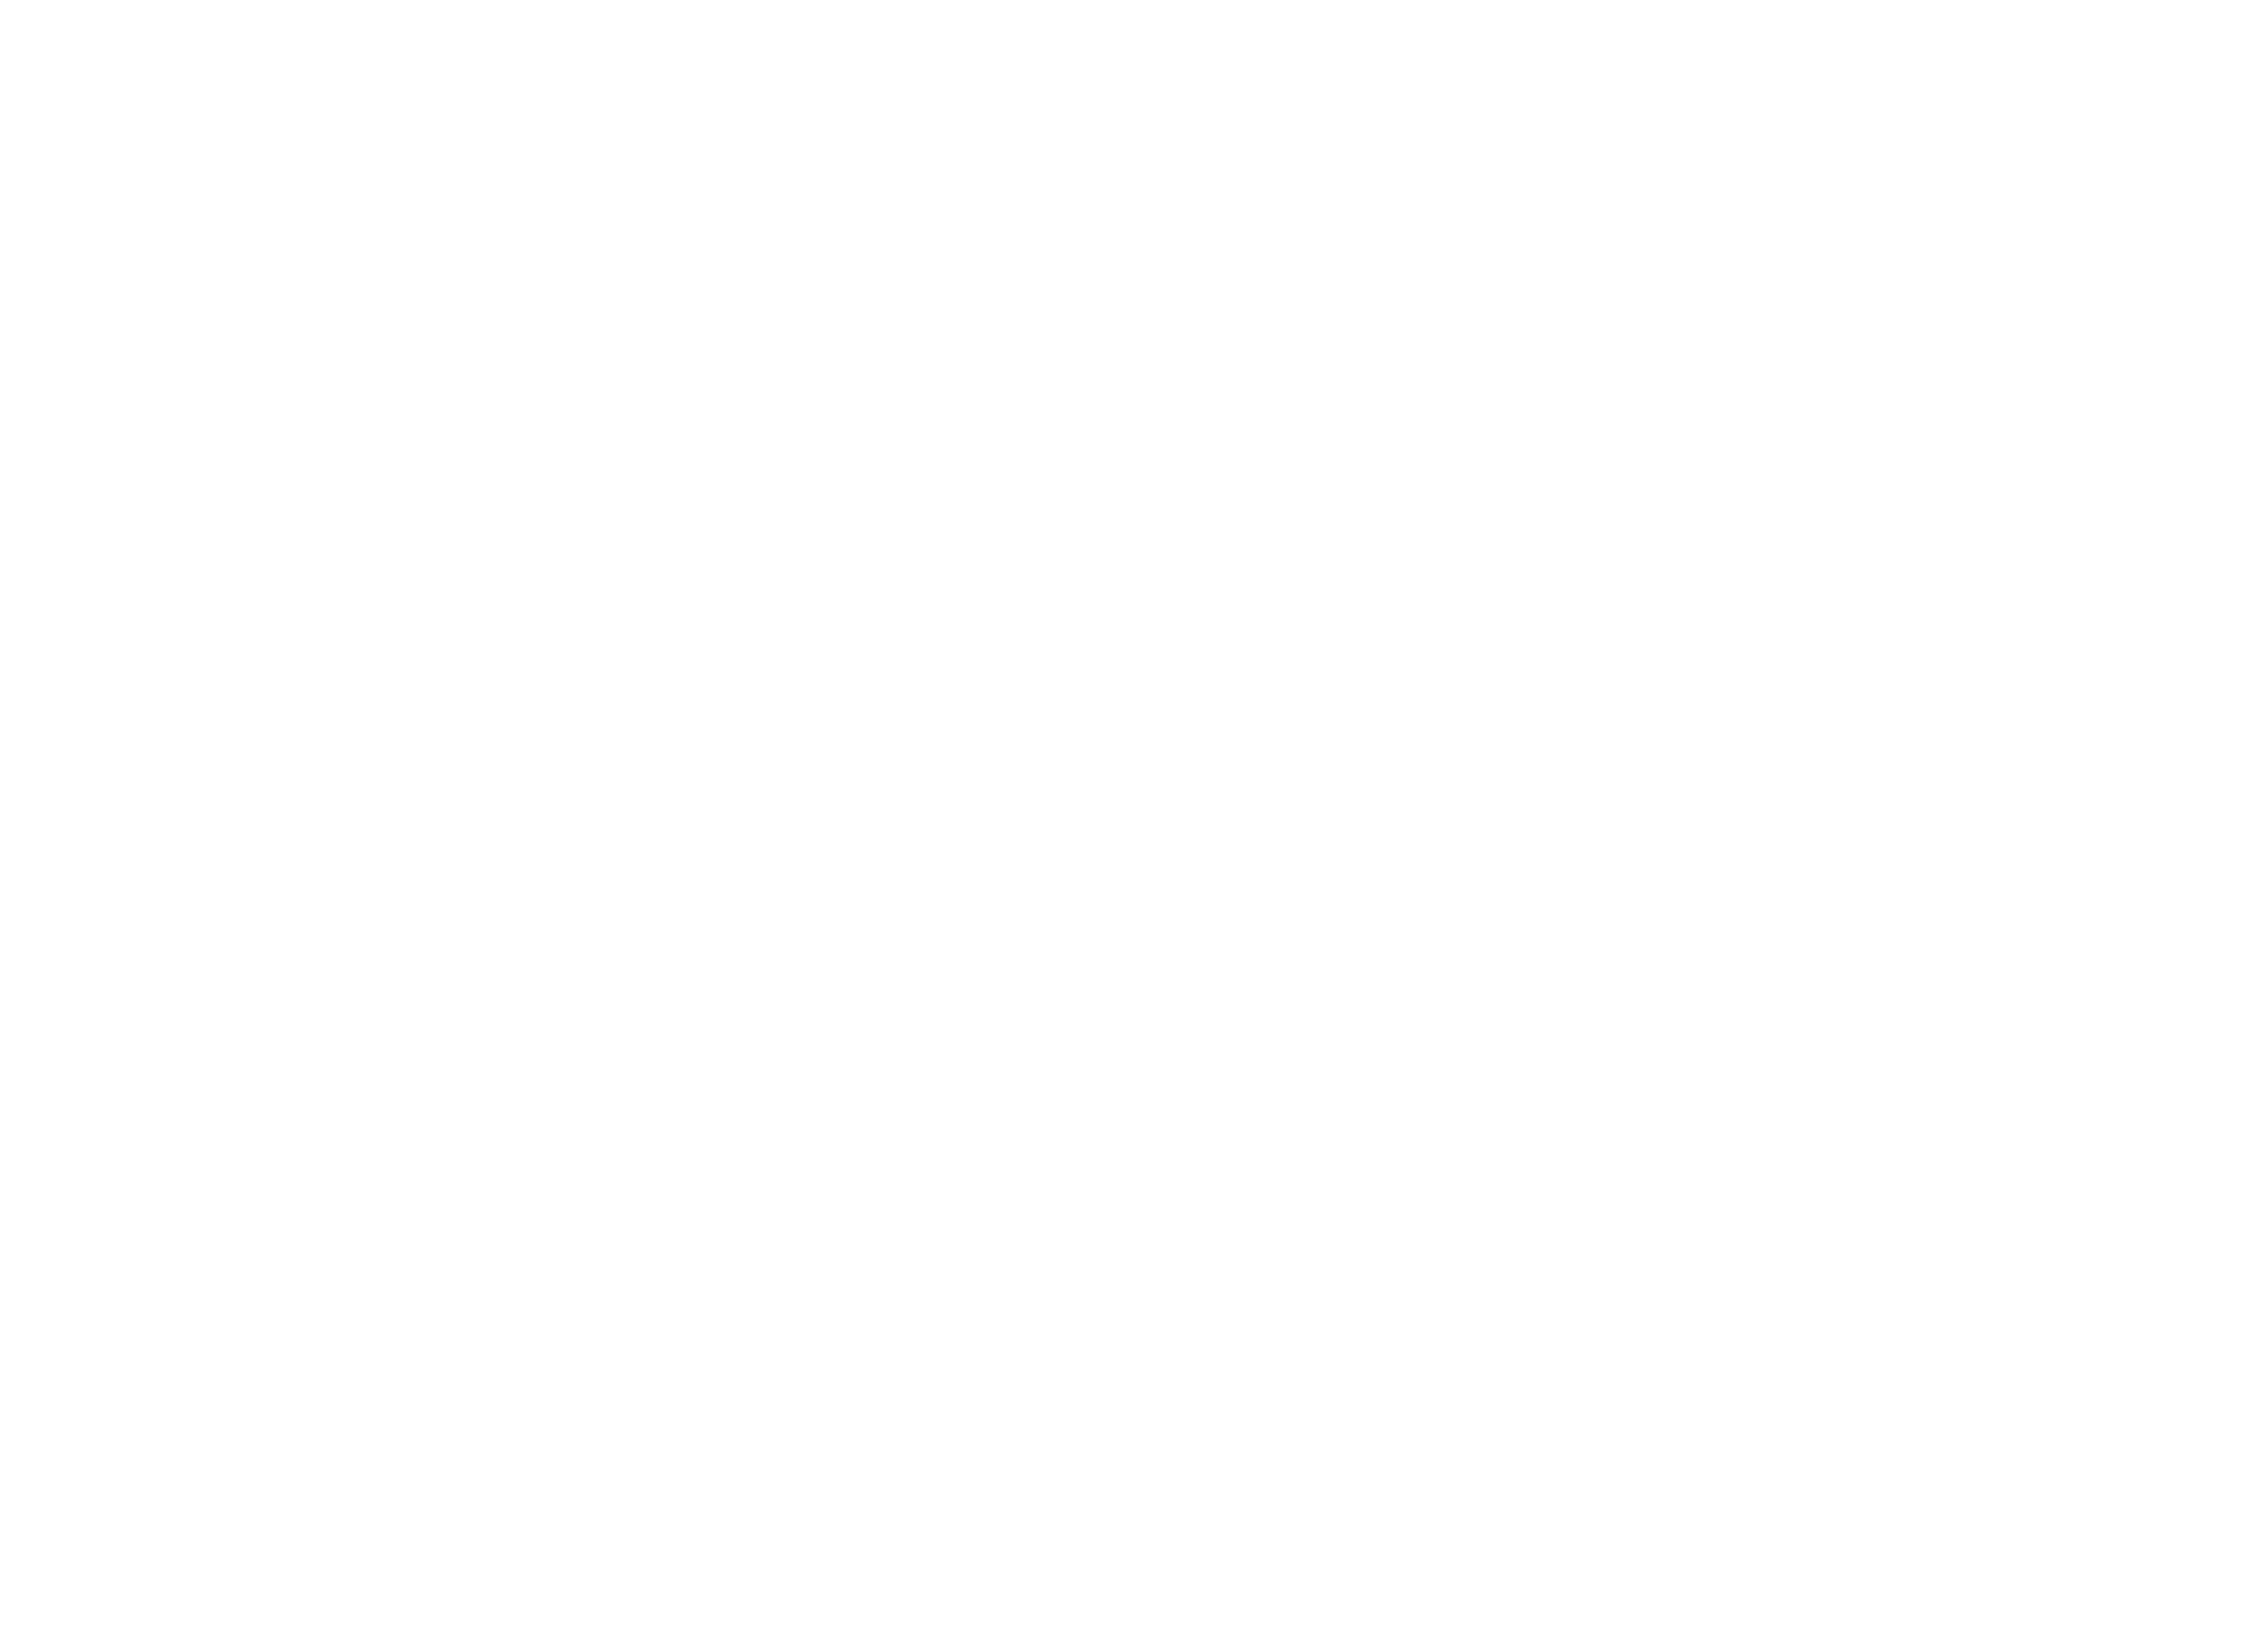
\includegraphics[width=0.45\textwidth]{Plots/ttV/dummy}
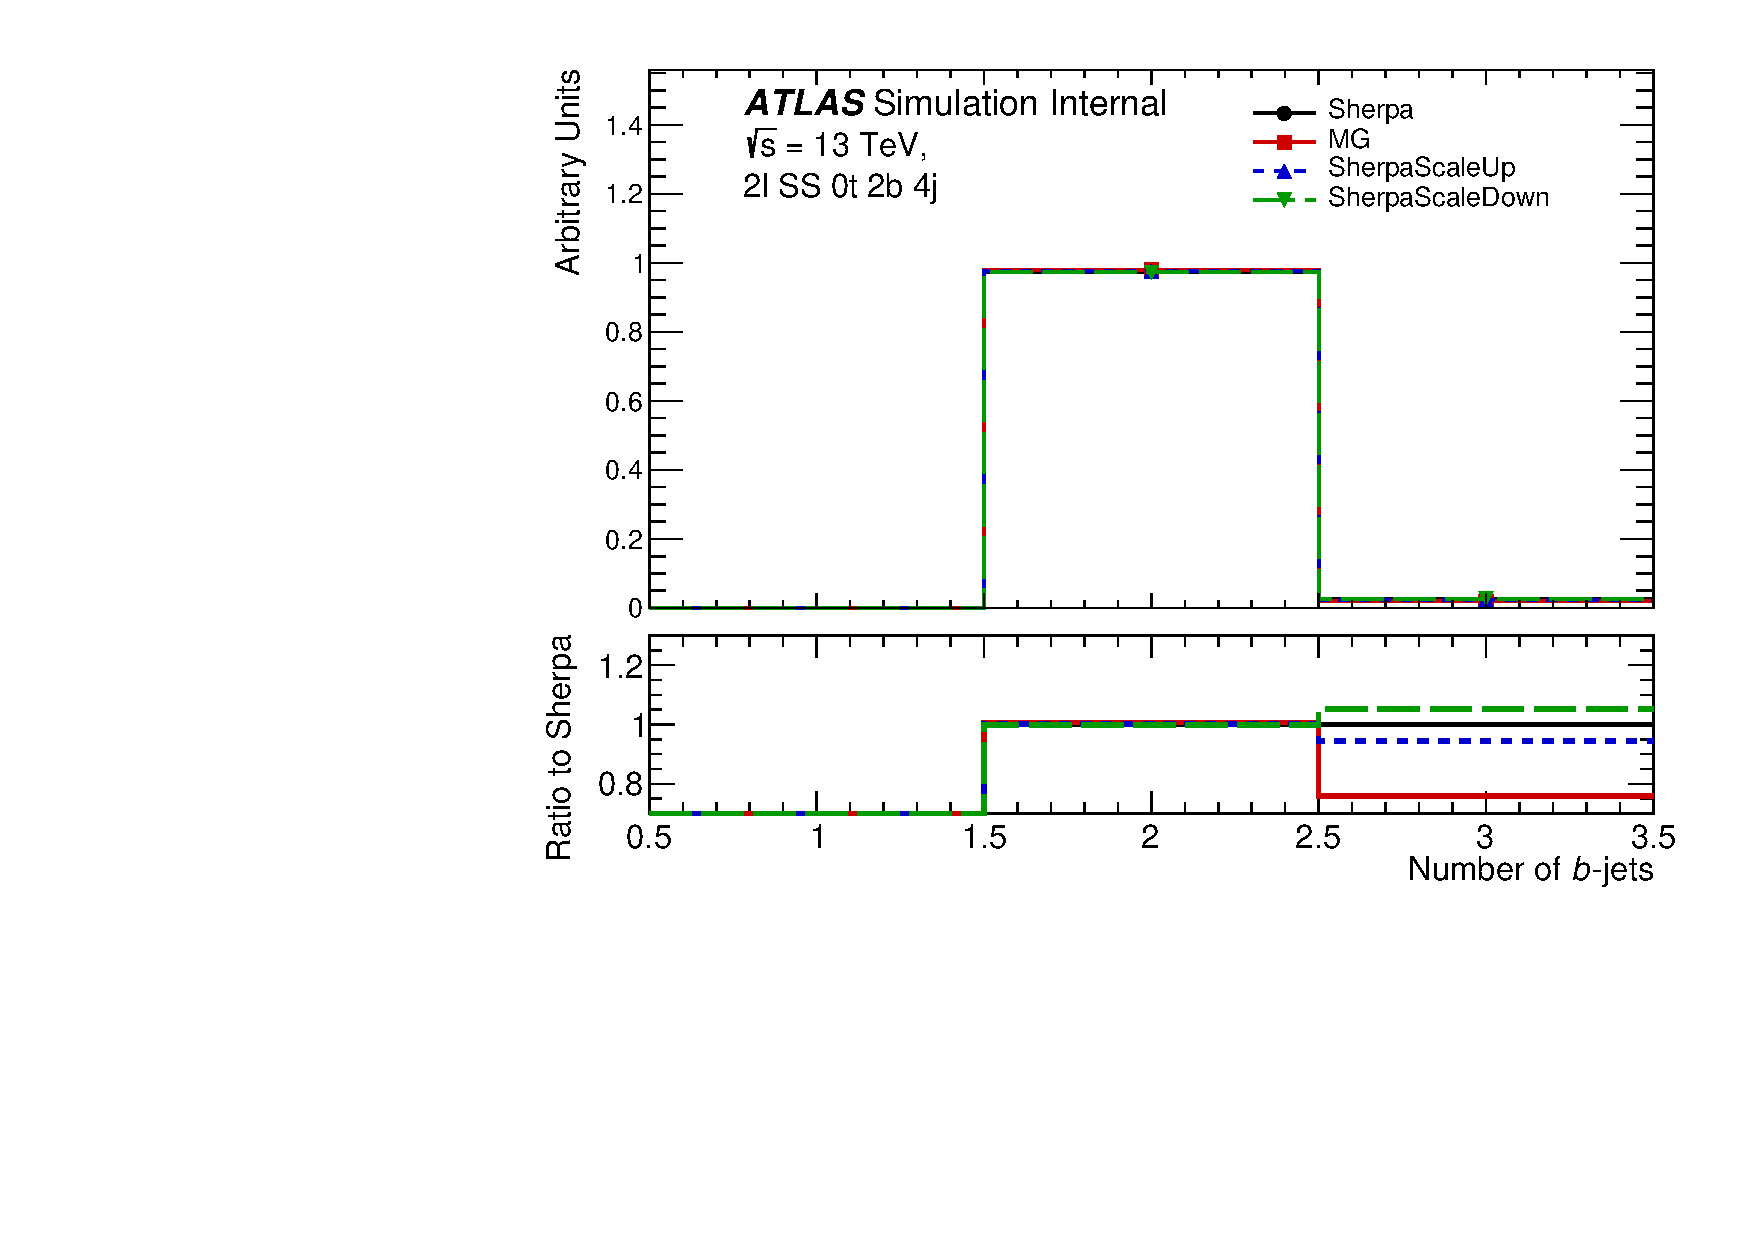
\includegraphics[width=0.45\textwidth]{Plots/ttV/shape/c_Region_1_nBtagJets}\\
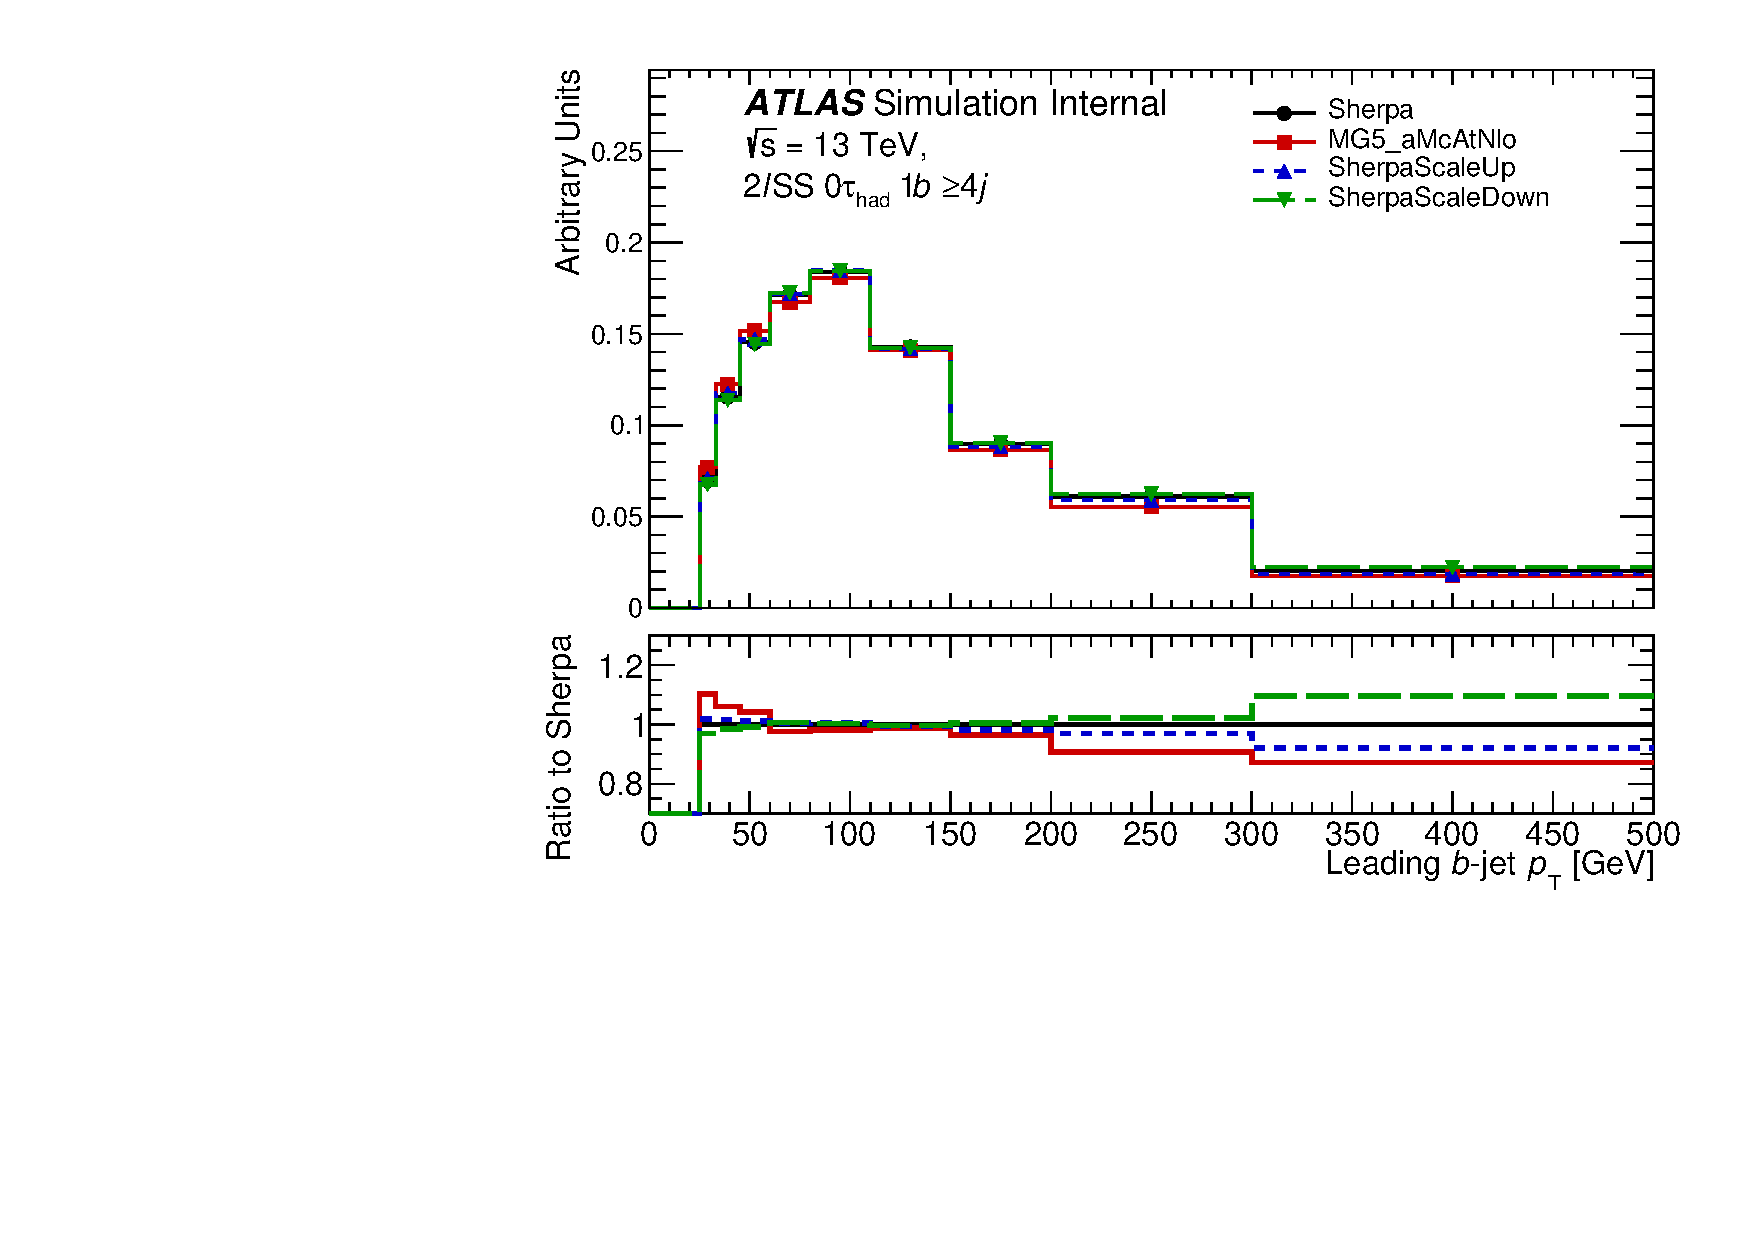
\includegraphics[width=0.45\textwidth]{Plots/ttV/shape/c_Region_0_Bjet_Pt_0}
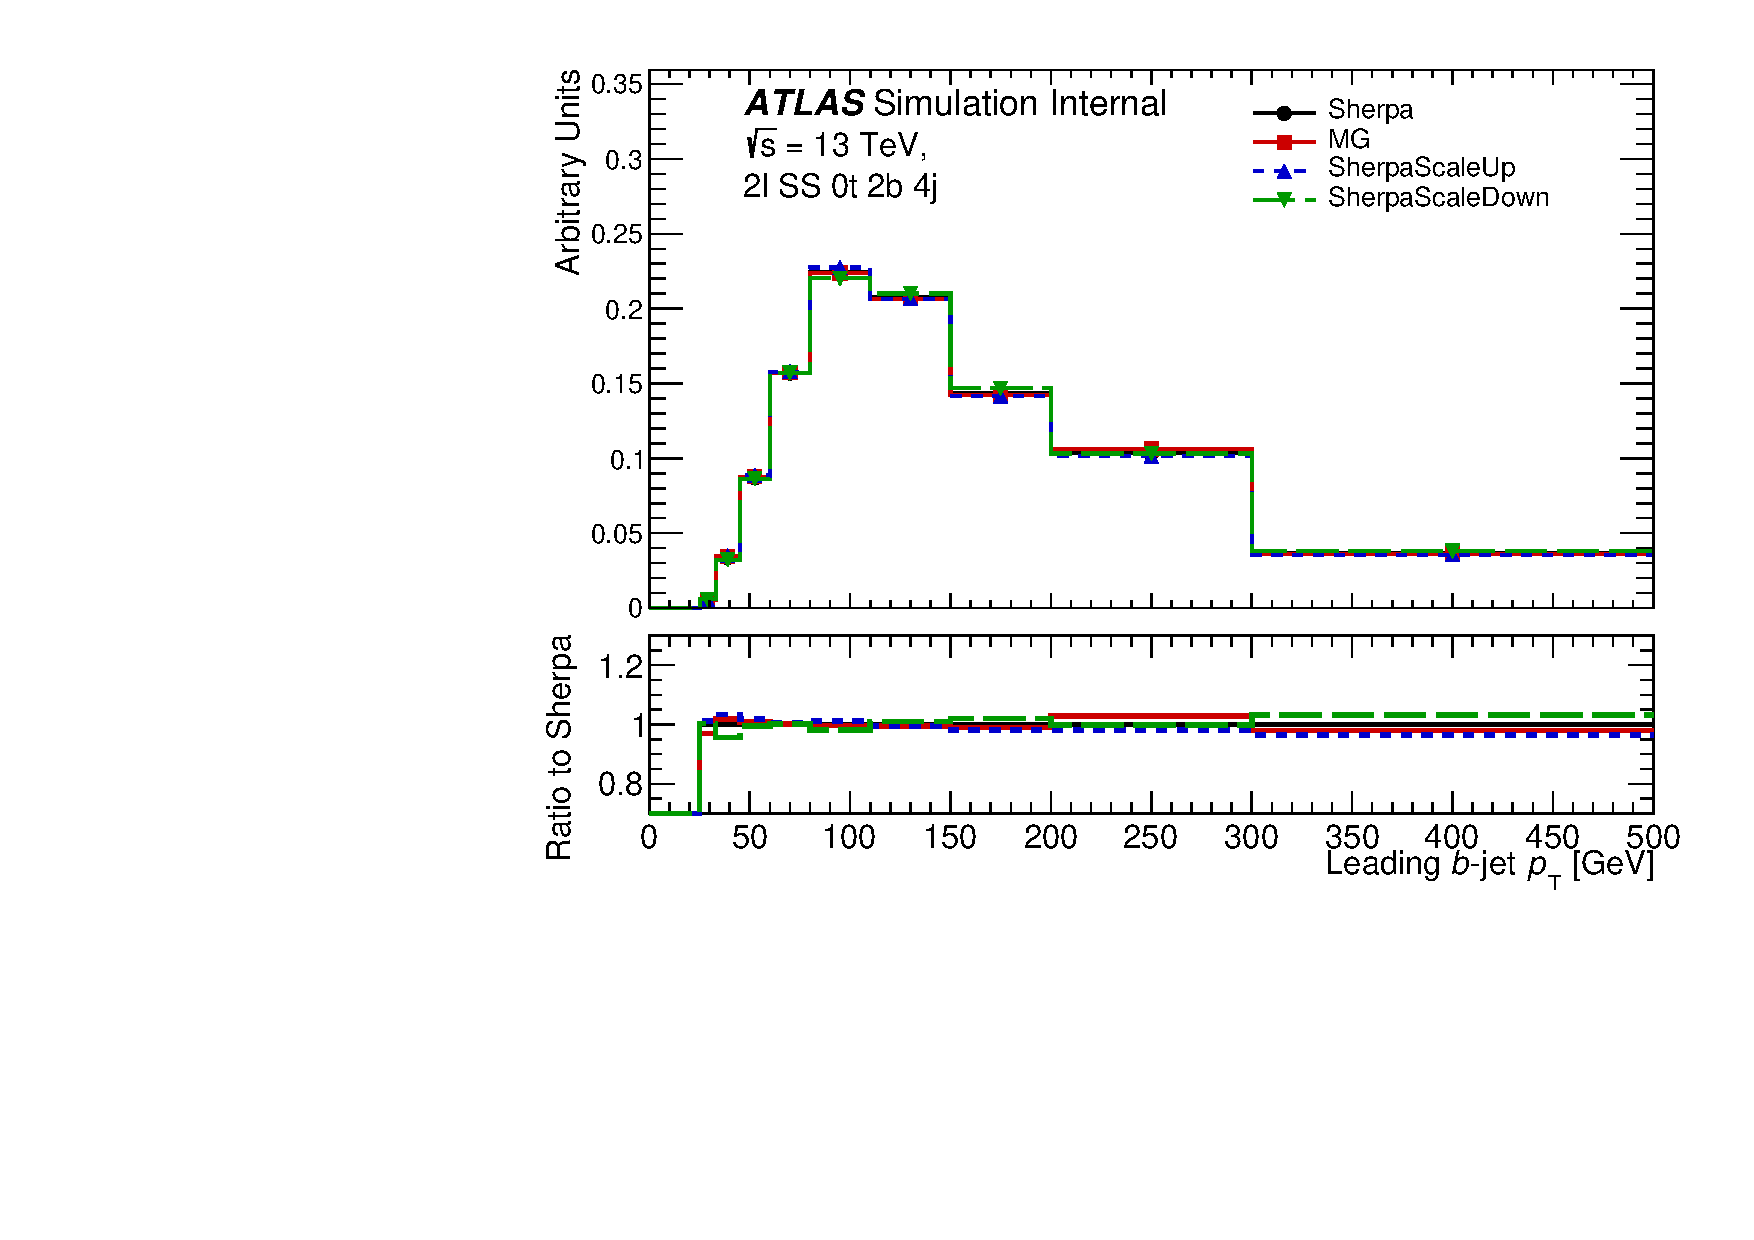
\includegraphics[width=0.45\textwidth]{Plots/ttV/shape/c_Region_1_Bjet_Pt_0}\\
  \caption{Distribution of the $b$-jet multiplicities (top) and the leading $b$-jet transverse momentum (bottom), for the Region 1 with 1$b$-jet (left) and Region 2 with 2$b$-jets (right) selection requiring four and more jets. Explanation in text. \label{ttV:4jbinfo}}
\end{figure}

Good agreement of the single lepton kinematics can be seen between nominal and alternative generators for $\geq2b$-jets selections, as presented in the right of Figures~\ref{ttV:lep_kin} (presented Region 2, while similar behaviour seen in Region 4 as well). 
%While there is an offset of the order of 10\%  between nominal and alternative generators for 1$b$-jet selections, as presented in the left of Figures~\ref{ttV:lep_kin} (Region 1 showed, while similar trend seen in Region 3 as well). 

Sizeable difference in shapes between nominal and alternative generators observed for the distributions corresponding to the correlations between two leptons such as the angular distance between the two leptons, maximum of lepton's pseudorapidity and azimuthal separation between the leptons, as illustrated in Figures~\ref{ttV:ll_kin} for Region 1 on the right and Region 2 on the left (similar trends observed in Regions 3 and 4).
%As was observed for single lepton kinematics, difference in 1$b$-jet selections is increased wrt to $\geq2b$-jets selection.
%Distributions are presented for $\geq2N_{b-jets},\geq4N_{jets}$ region, while similar behaviour seen in all other regions as well.

Distributions of the jet multiplicity, number of $b$-jets, the leading lepton transverse momentum and the angular distance between the two leptons  $\Delta R _{\ell \ell }$ for the Region 5 with 1$\tau_{had}$ selection are presented on Figure~\ref{ttV:tauR_kin}.
The difference observed between nominal and alternative generators for high jet multiplicities, at the edge of the scale variation uncertainty band. 
The distribution of $b$-jets agrees for $N_{b-jets}$ equal to two, and has sizeable difference in the 1$b$-jet bin, similarly to 0$\tau_{had}$ selections.
Lepton kinematic distributions has difference in shapes between nominal and alternative generators.

\begin{figure}[!htb]
\centering
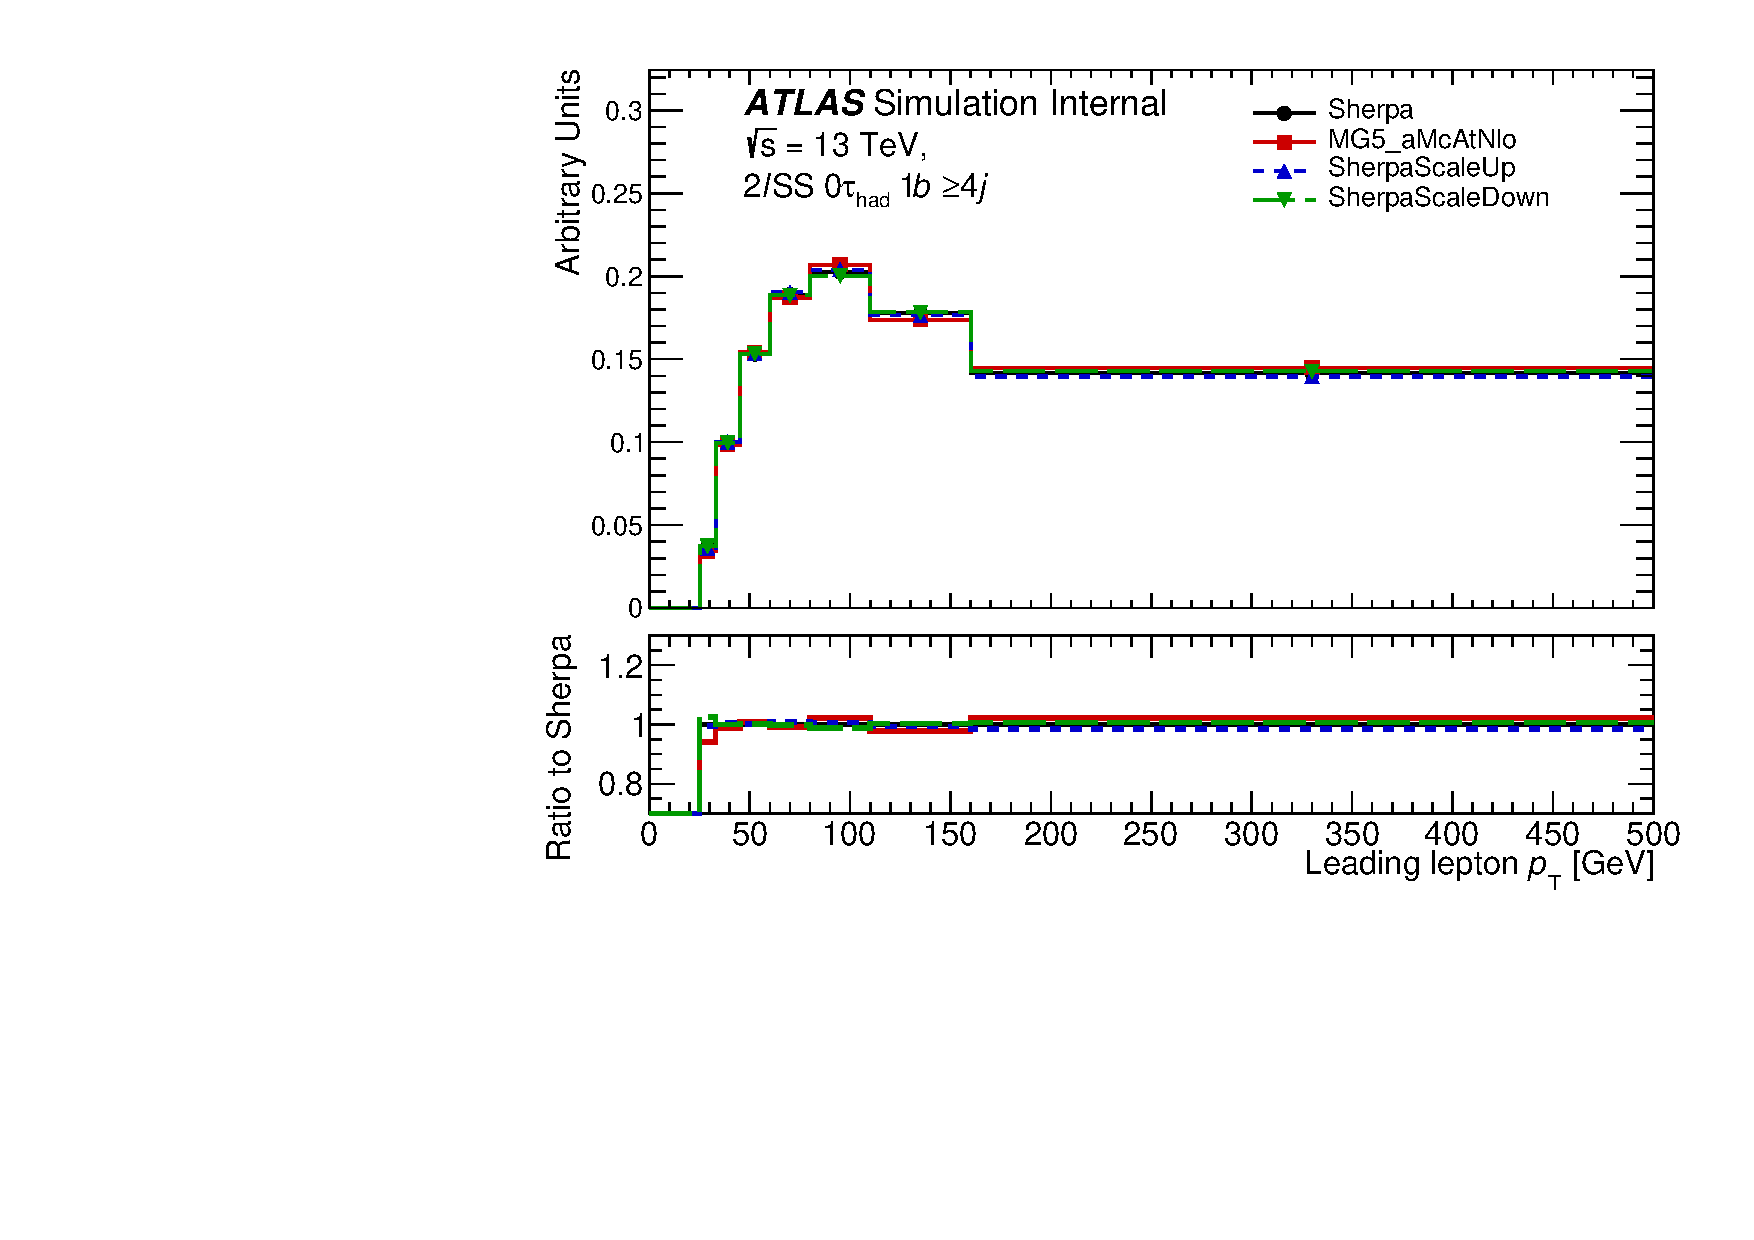
\includegraphics[width=0.45\textwidth]{Plots/ttV/shape/c_Region_0_lep_Pt_0}
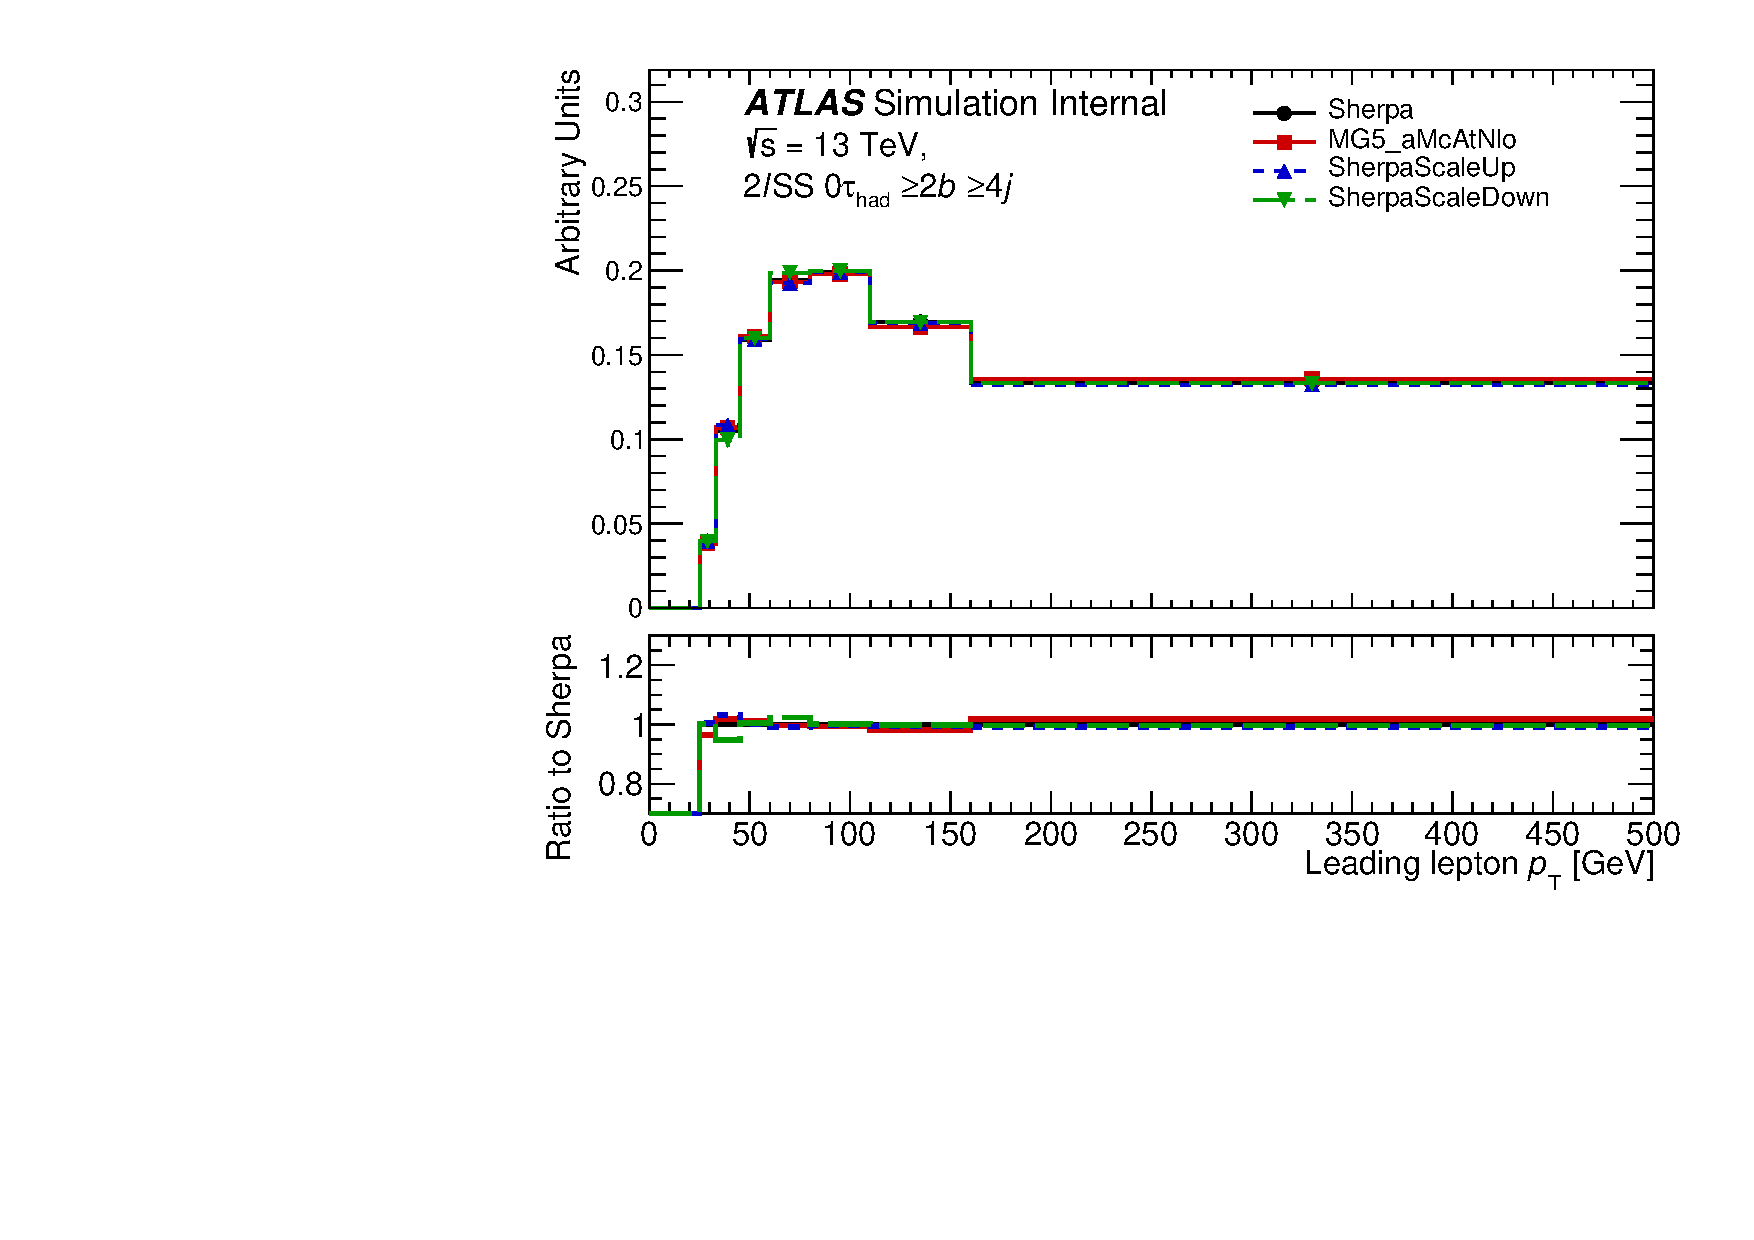
\includegraphics[width=0.45\textwidth]{Plots/ttV/shape/c_Region_1_lep_Pt_0}\\
%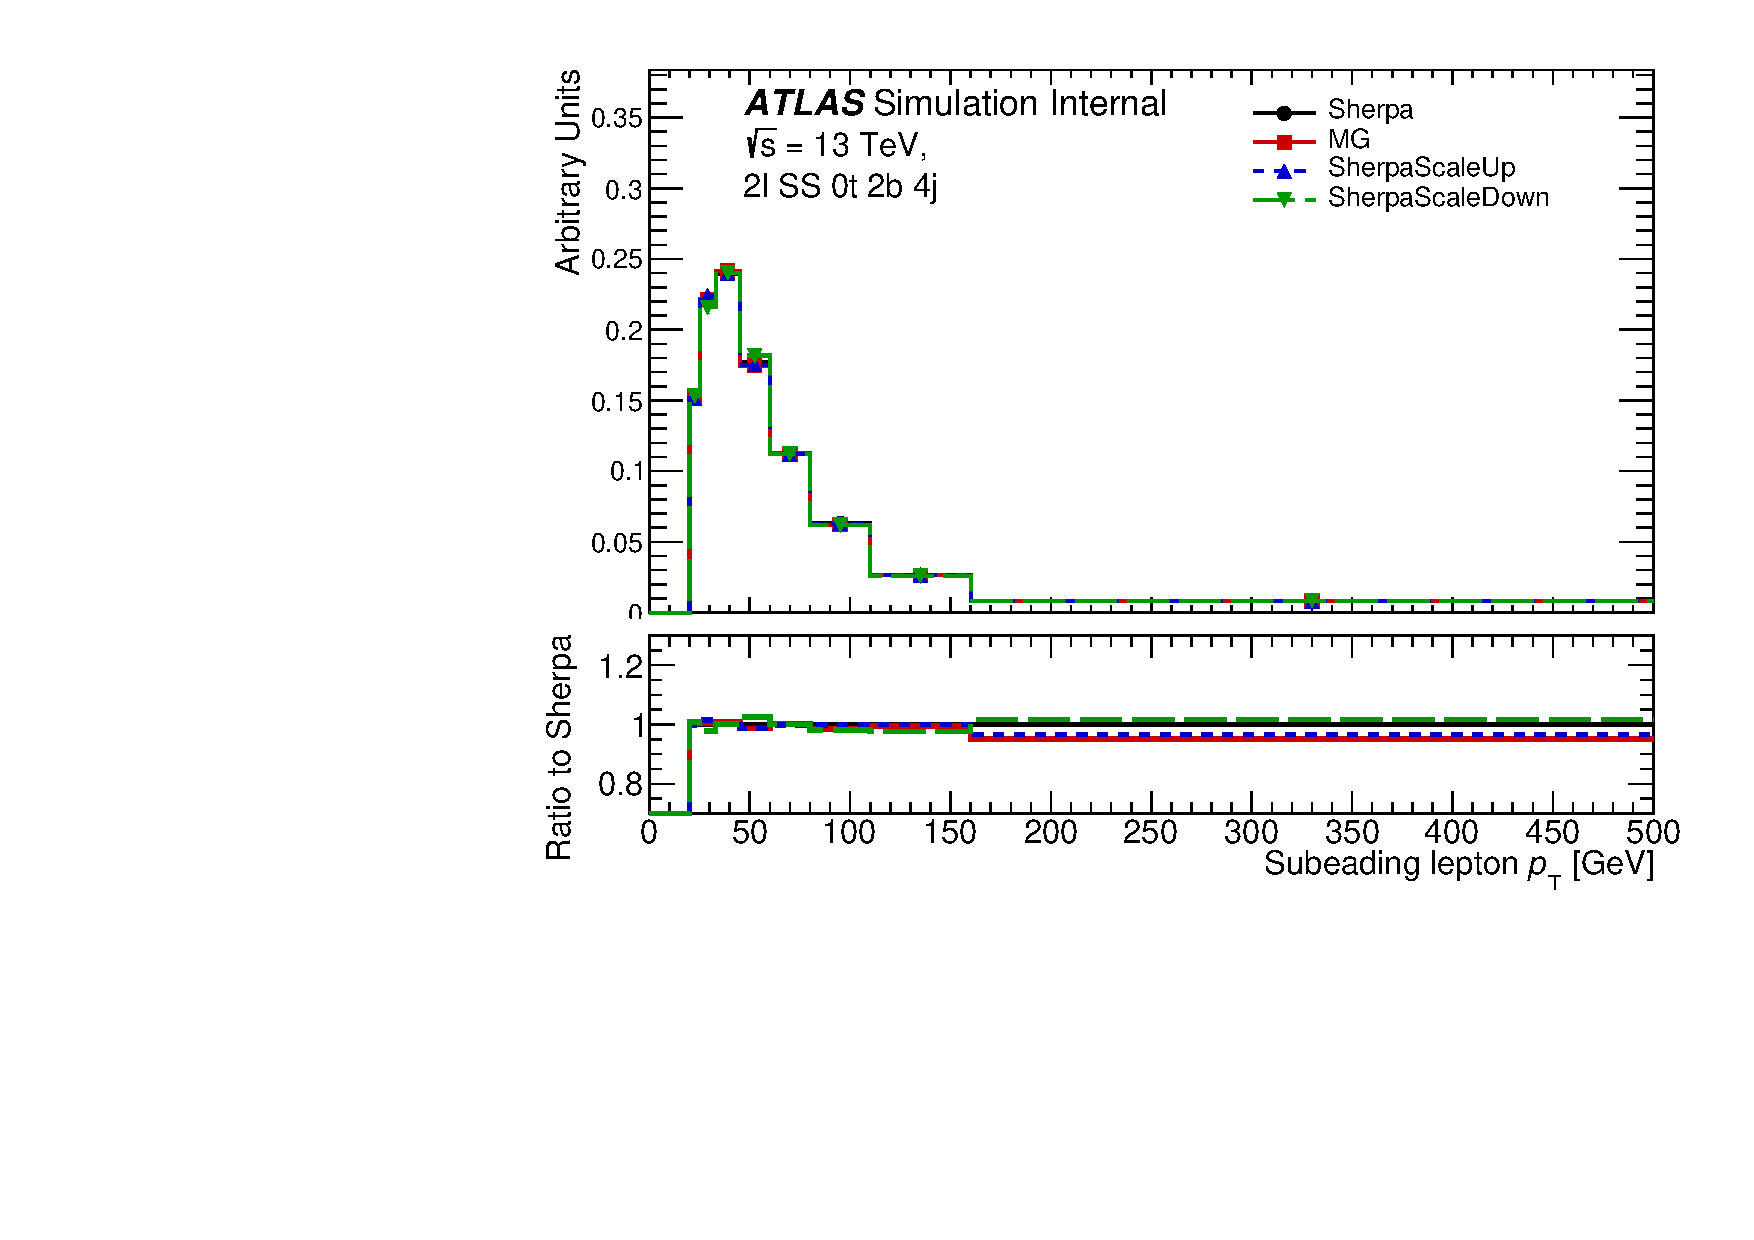
\includegraphics[width=0.45\textwidth]{Plots/ttV/shape/c_Region_1_lep_Pt_1}
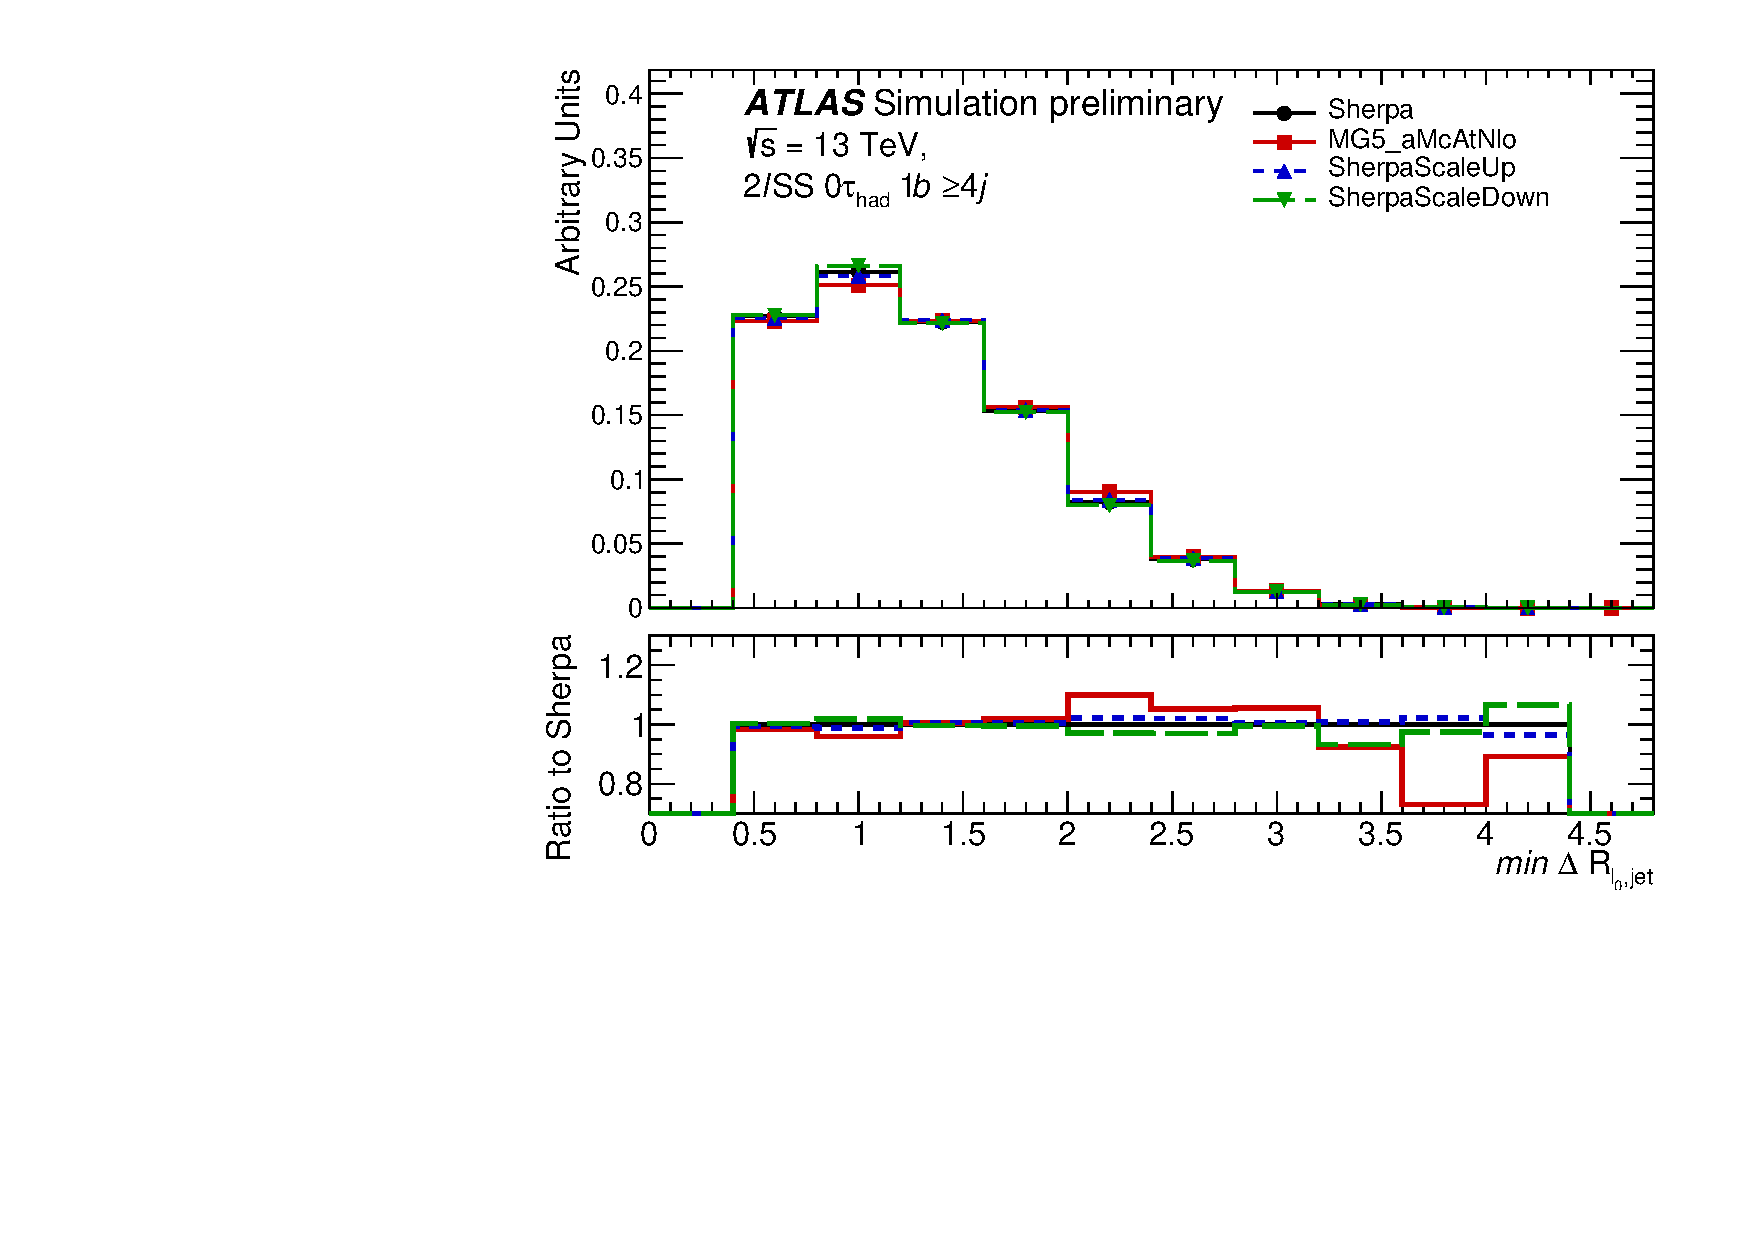
\includegraphics[width=0.45\textwidth]{Plots/ttV/shape/c_Region_0_min_DRl0j}
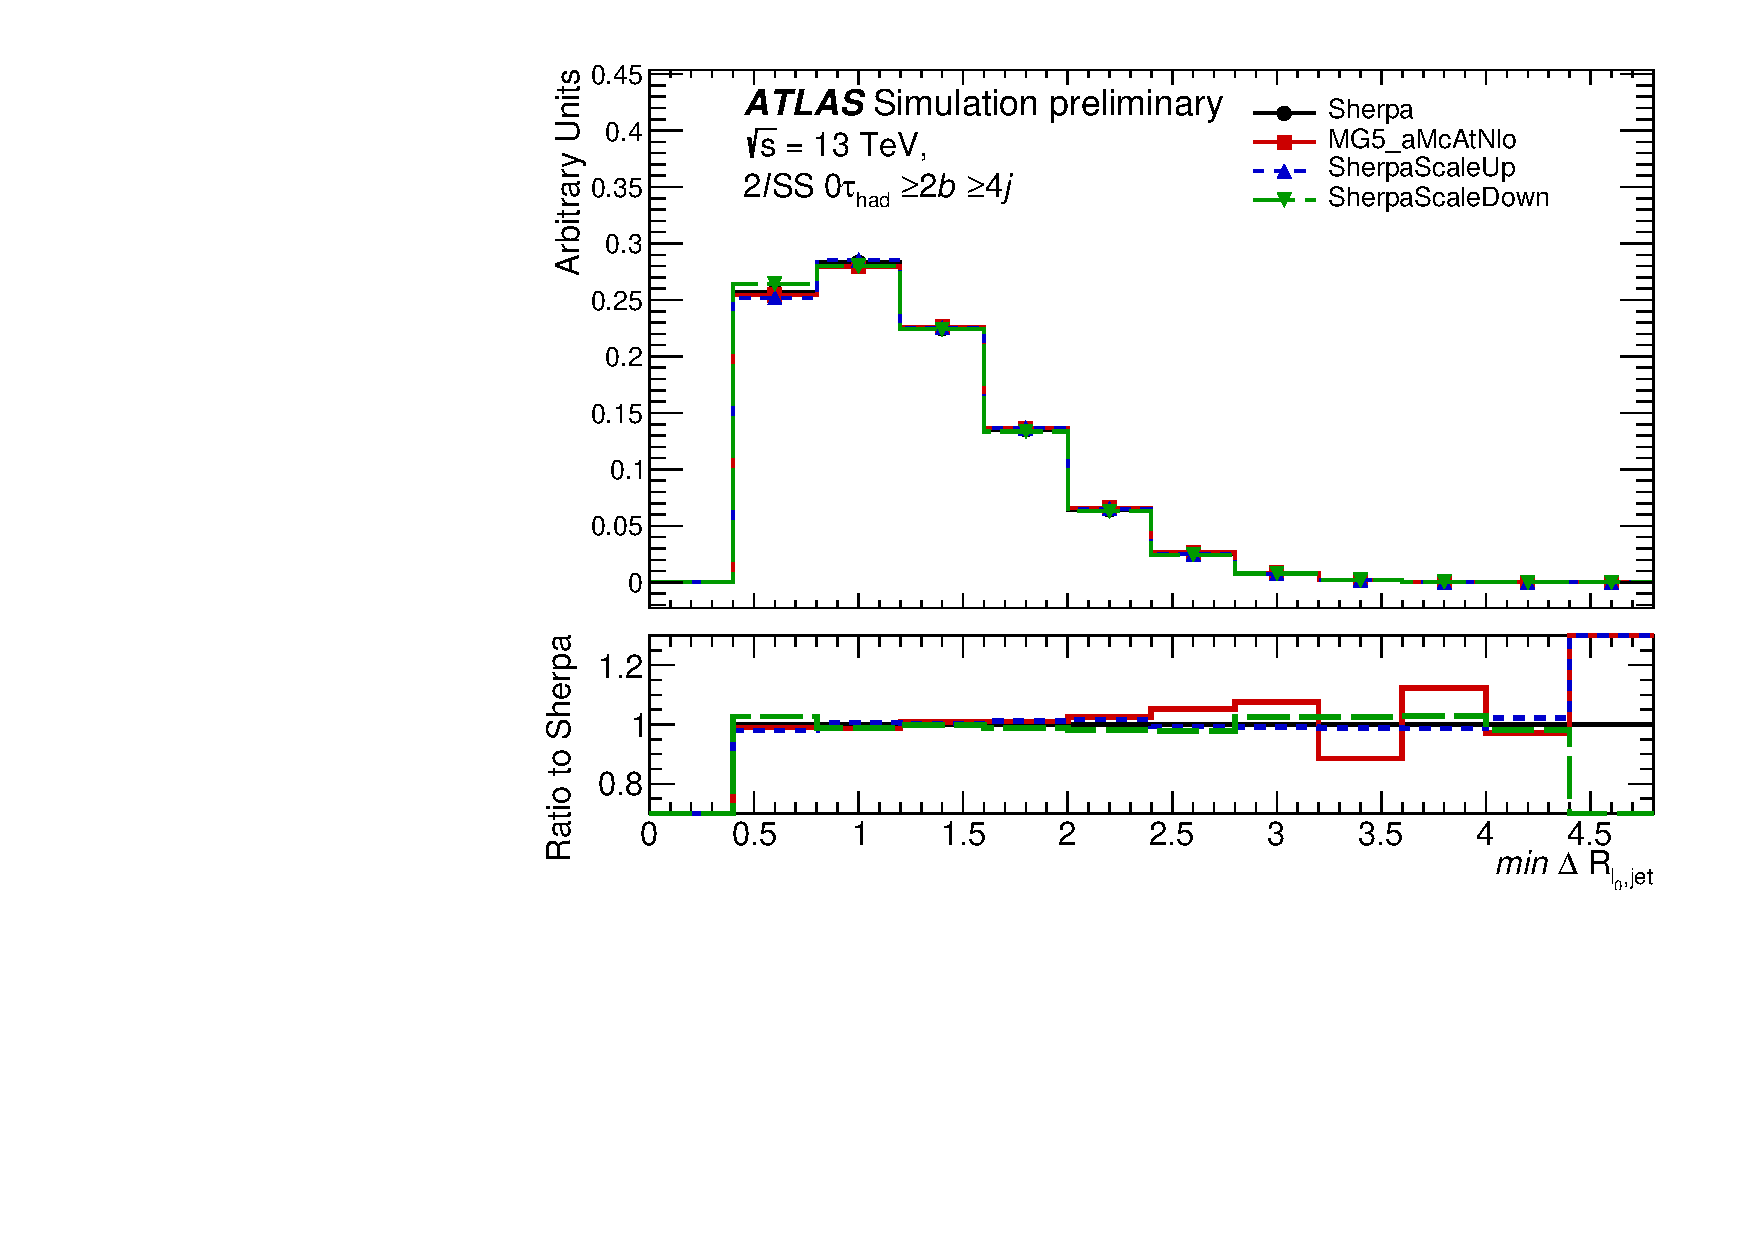
\includegraphics[width=0.45\textwidth]{Plots/ttV/shape/c_Region_1_min_DRl0j}\\
  \caption{Distribution of the leading lepton transverse momentum (top) and the minimum angular separation between the leading lepton and the nearest jet (bottom), for the Region 1 with 1$b$-jet (left) and Region 2 with 2$b$-jets (right) selection requiring four and more jets. Explanation in text.
  \label{ttV:lep_kin}}
\end{figure}

\begin{figure}[!htb]
\centering
	% \hspace{25mm} $DRl_0l_1$  \hspace{20mm} $max|\eta^{\ell\ell}|$\\
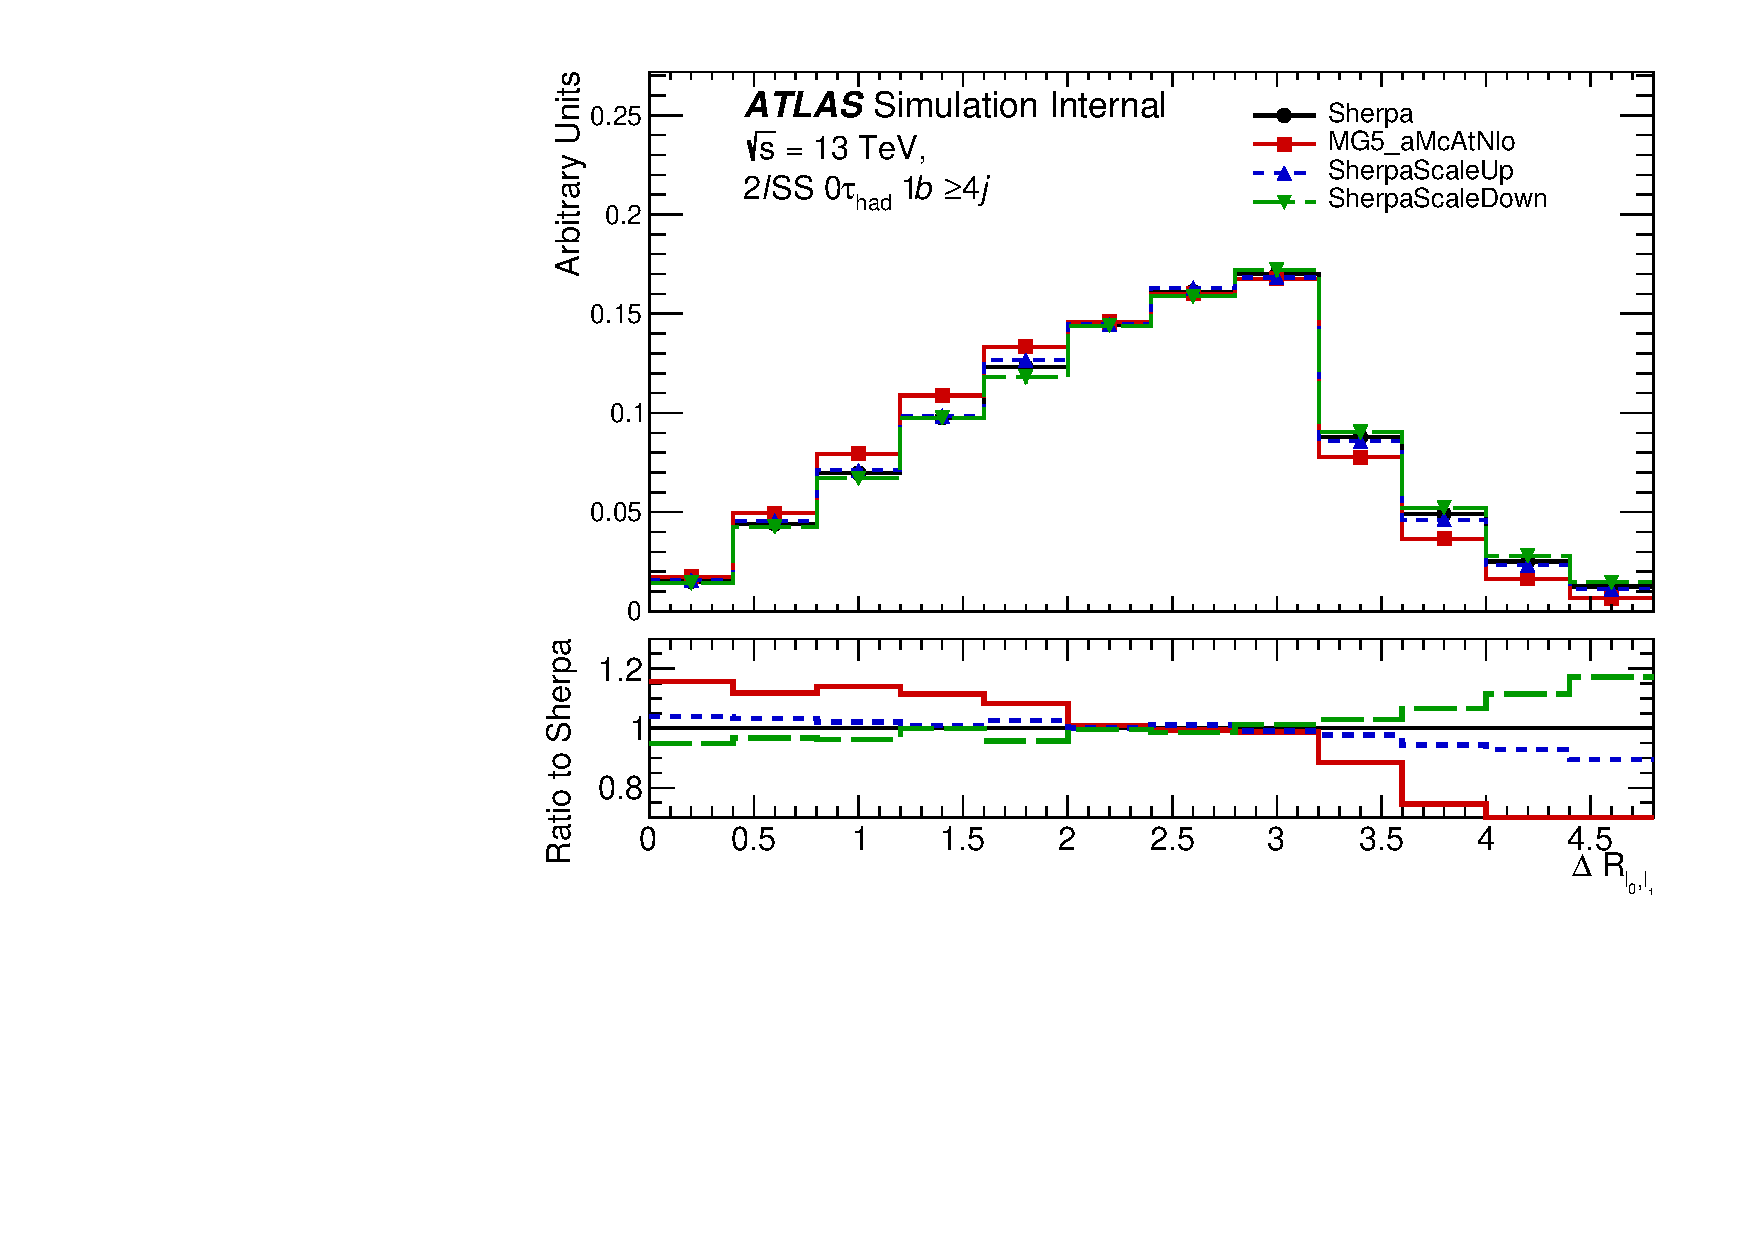
\includegraphics[width=0.45\textwidth]{Plots/ttV/shape/c_Region_0_DRll01}
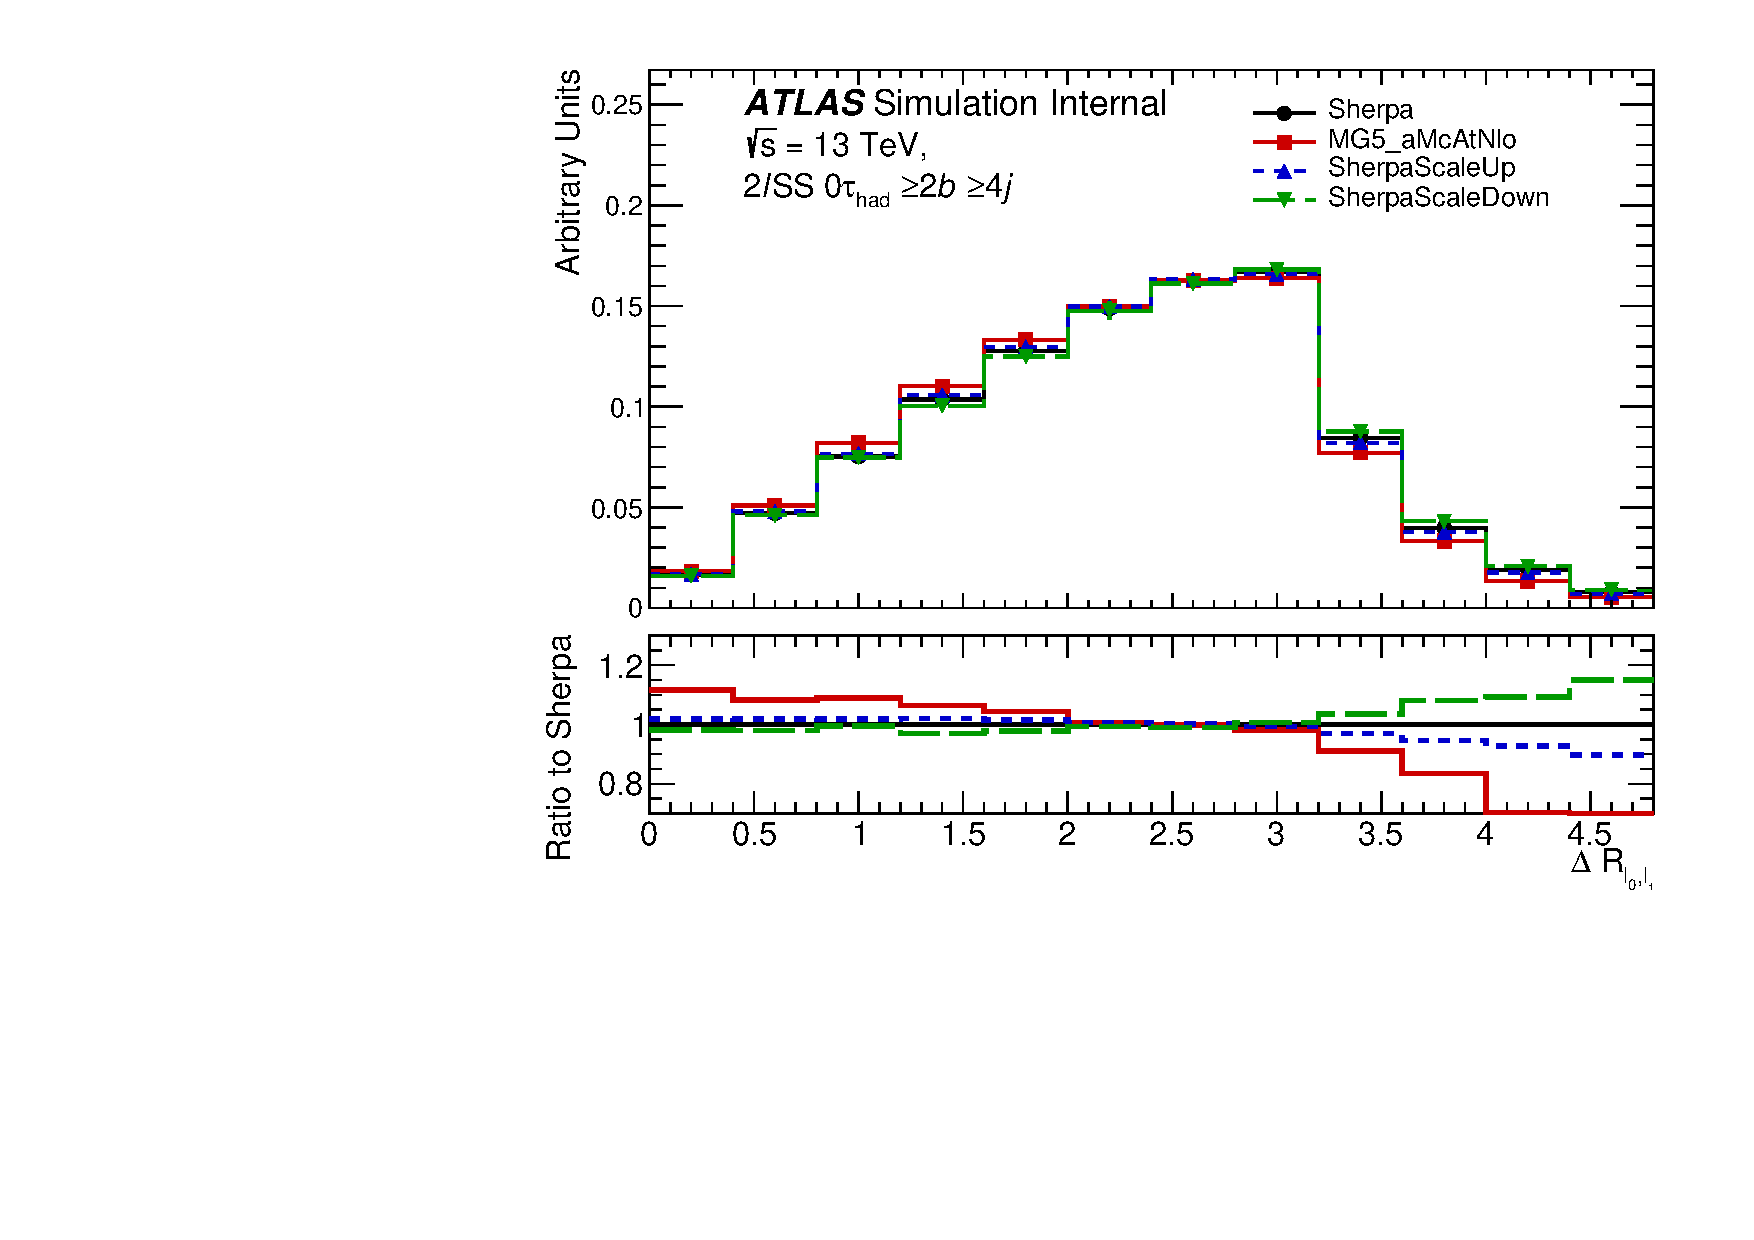
\includegraphics[width=0.45\textwidth]{Plots/ttV/shape/c_Region_1_DRll01}\\
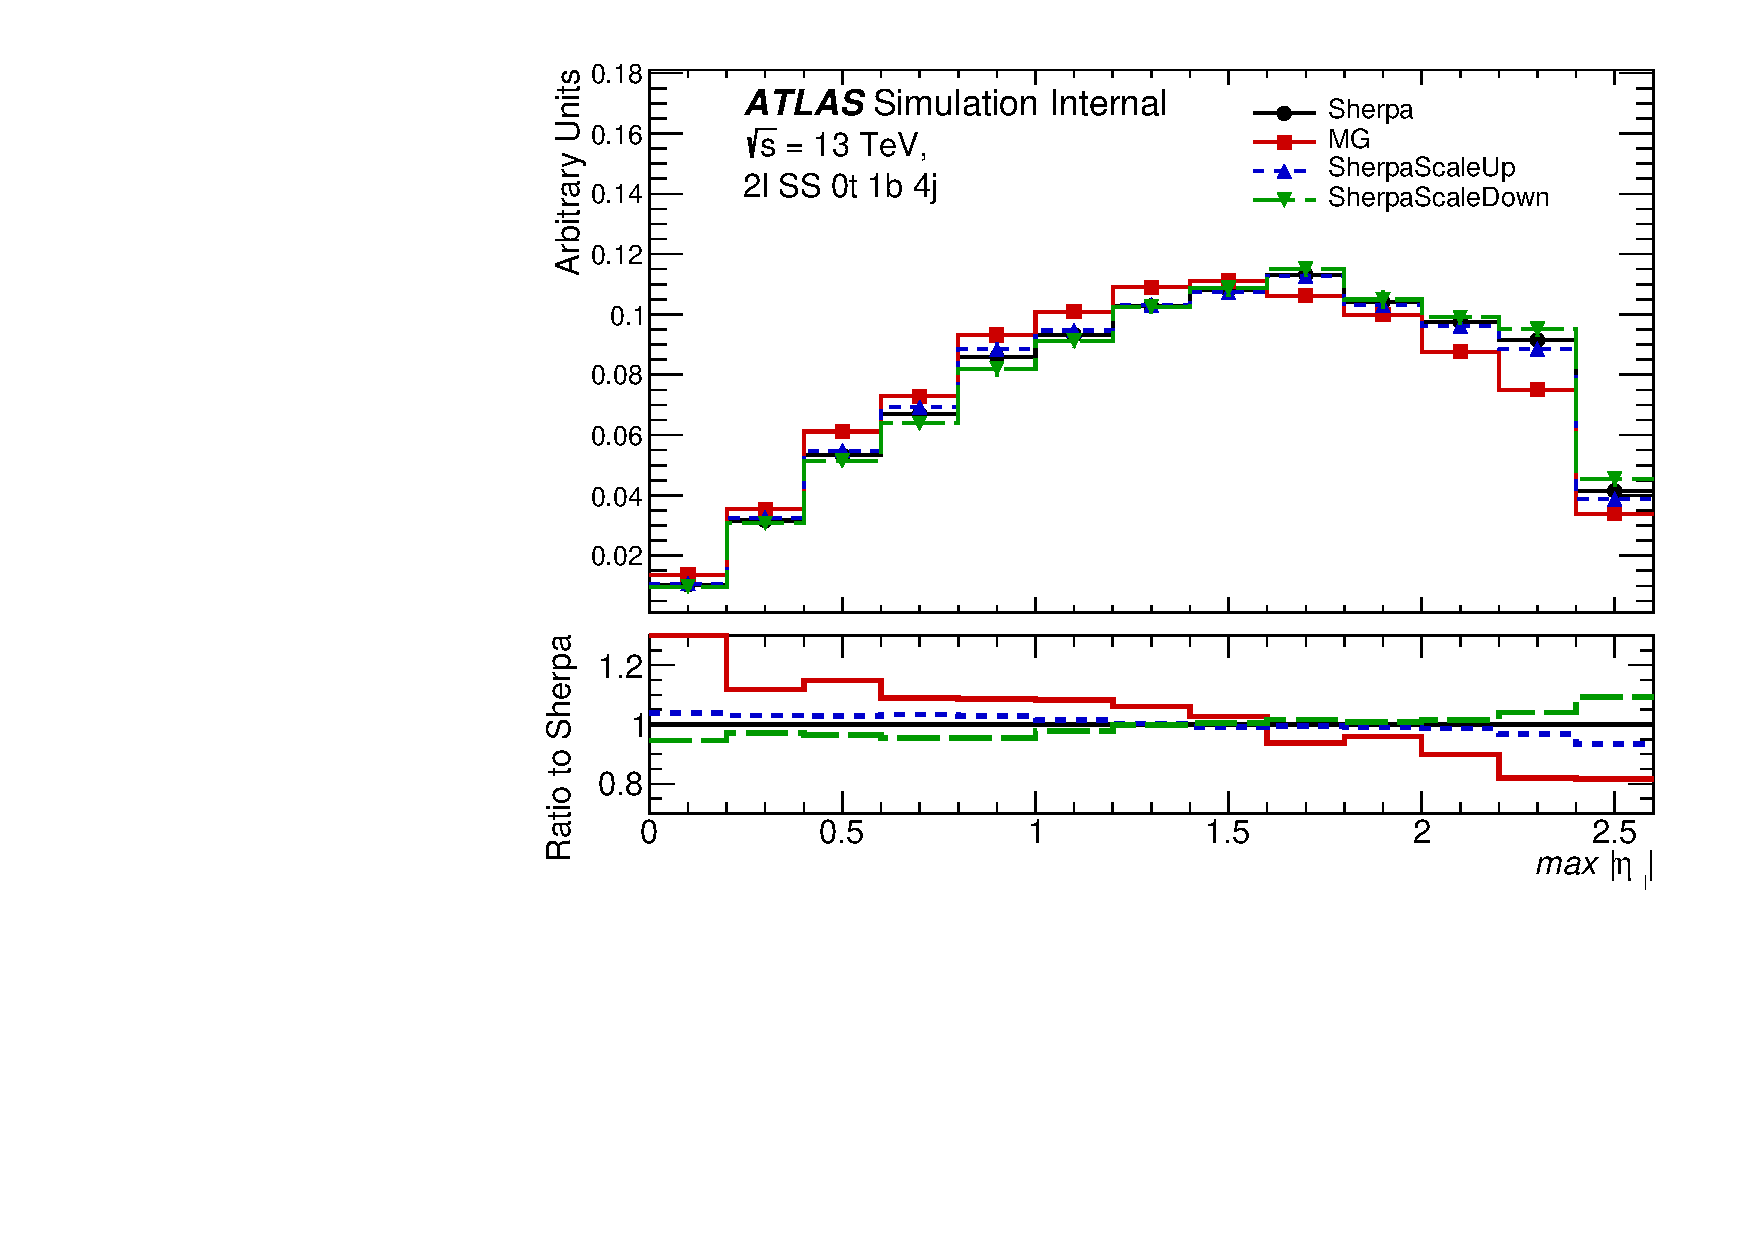
\includegraphics[width=0.45\textwidth]{Plots/ttV/shape/c_Region_0_maxEta_ll} 
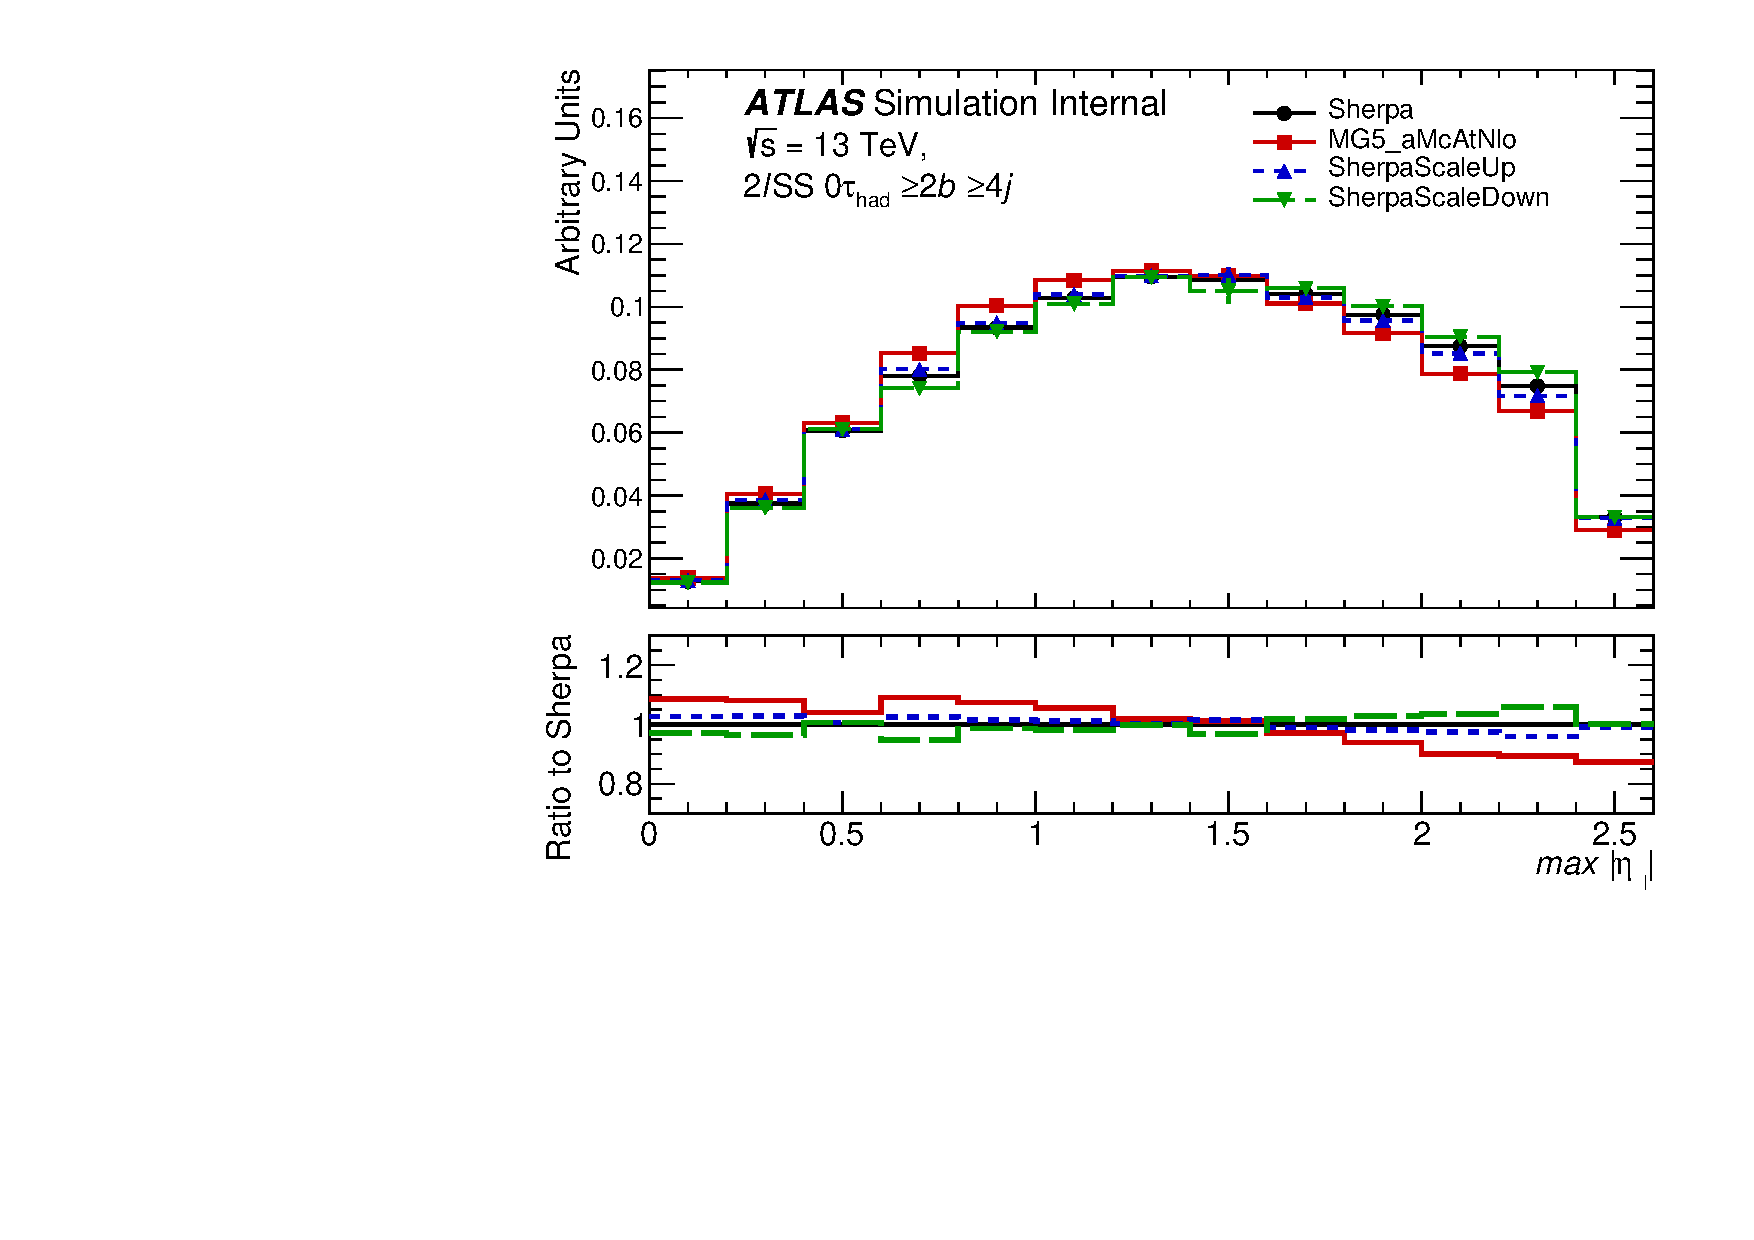
\includegraphics[width=0.45\textwidth]{Plots/ttV/shape/c_Region_1_maxEta_ll}\\
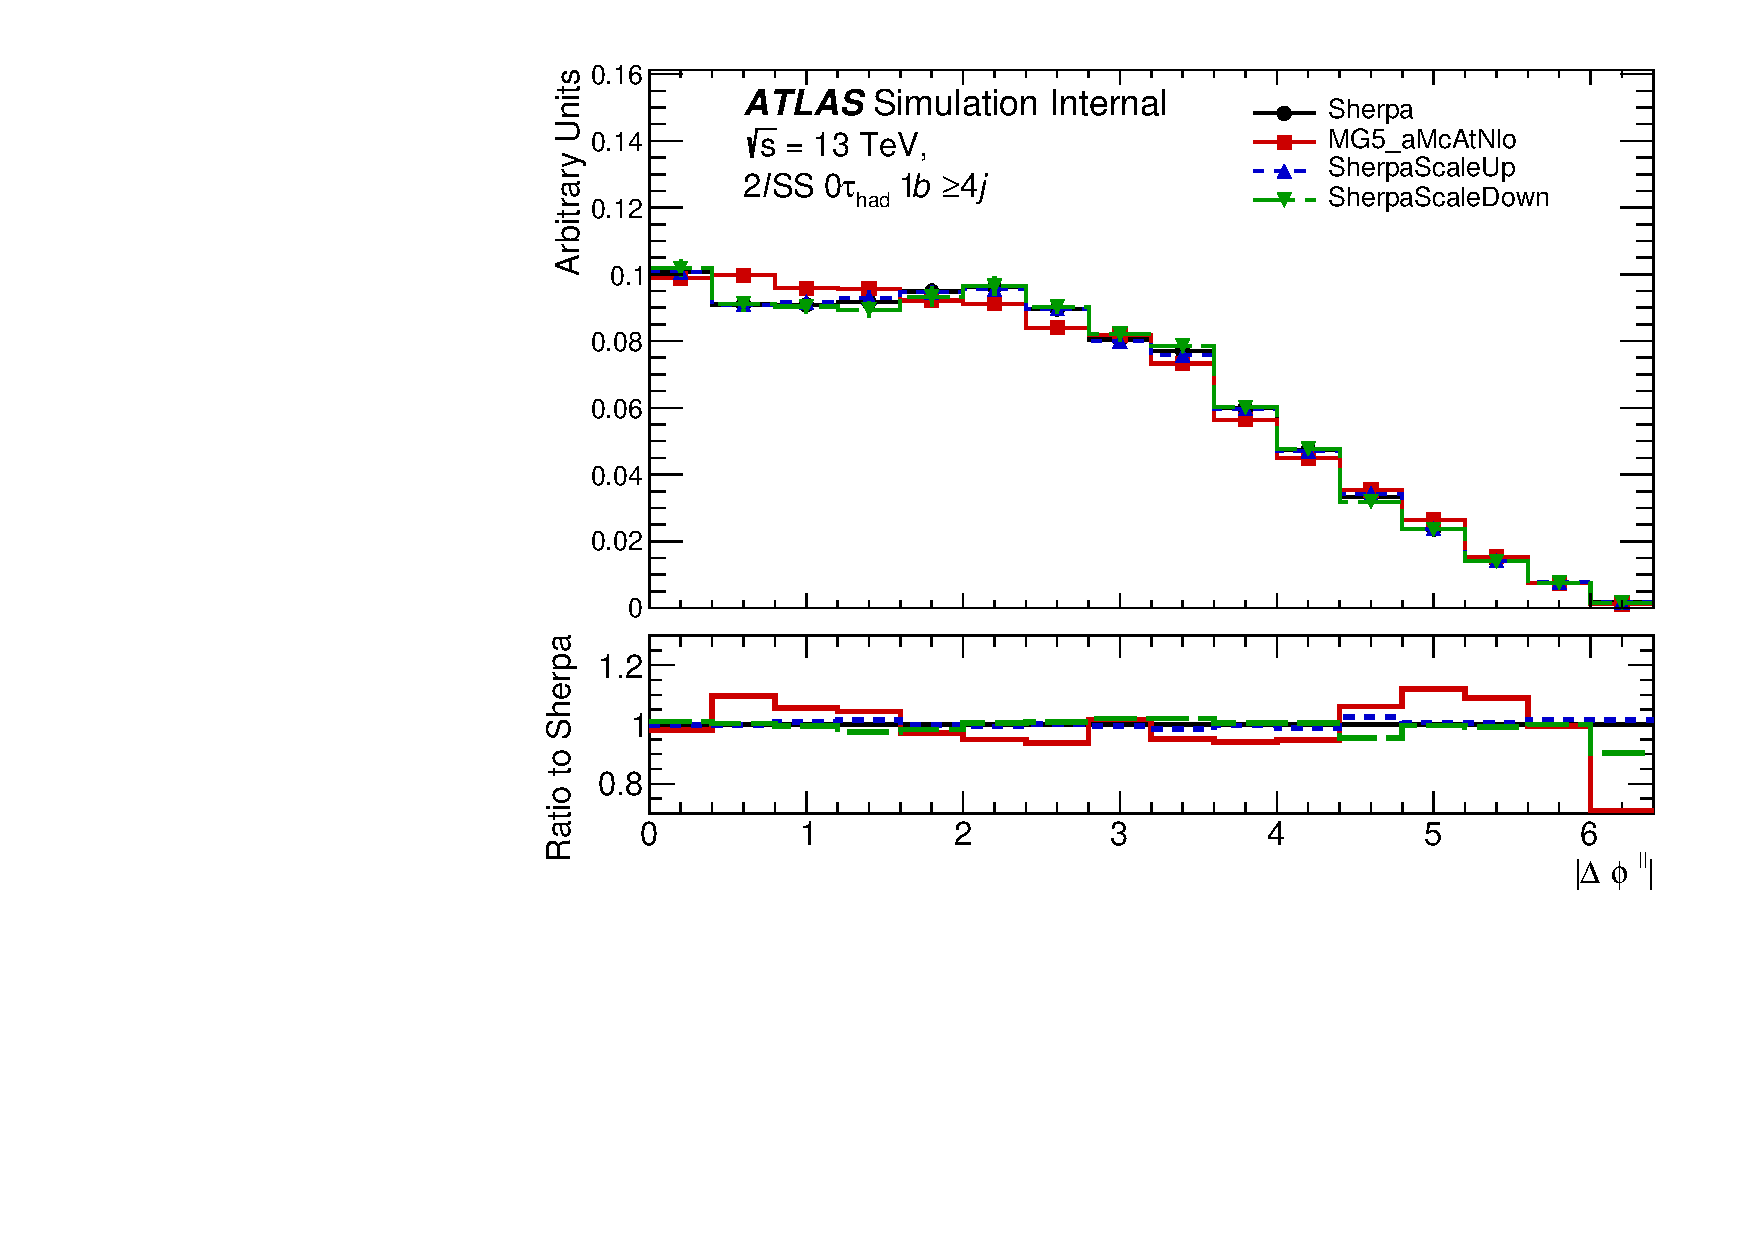
\includegraphics[width=0.45\textwidth]{Plots/ttV/shape/c_Region_0_lep_dPhi} 
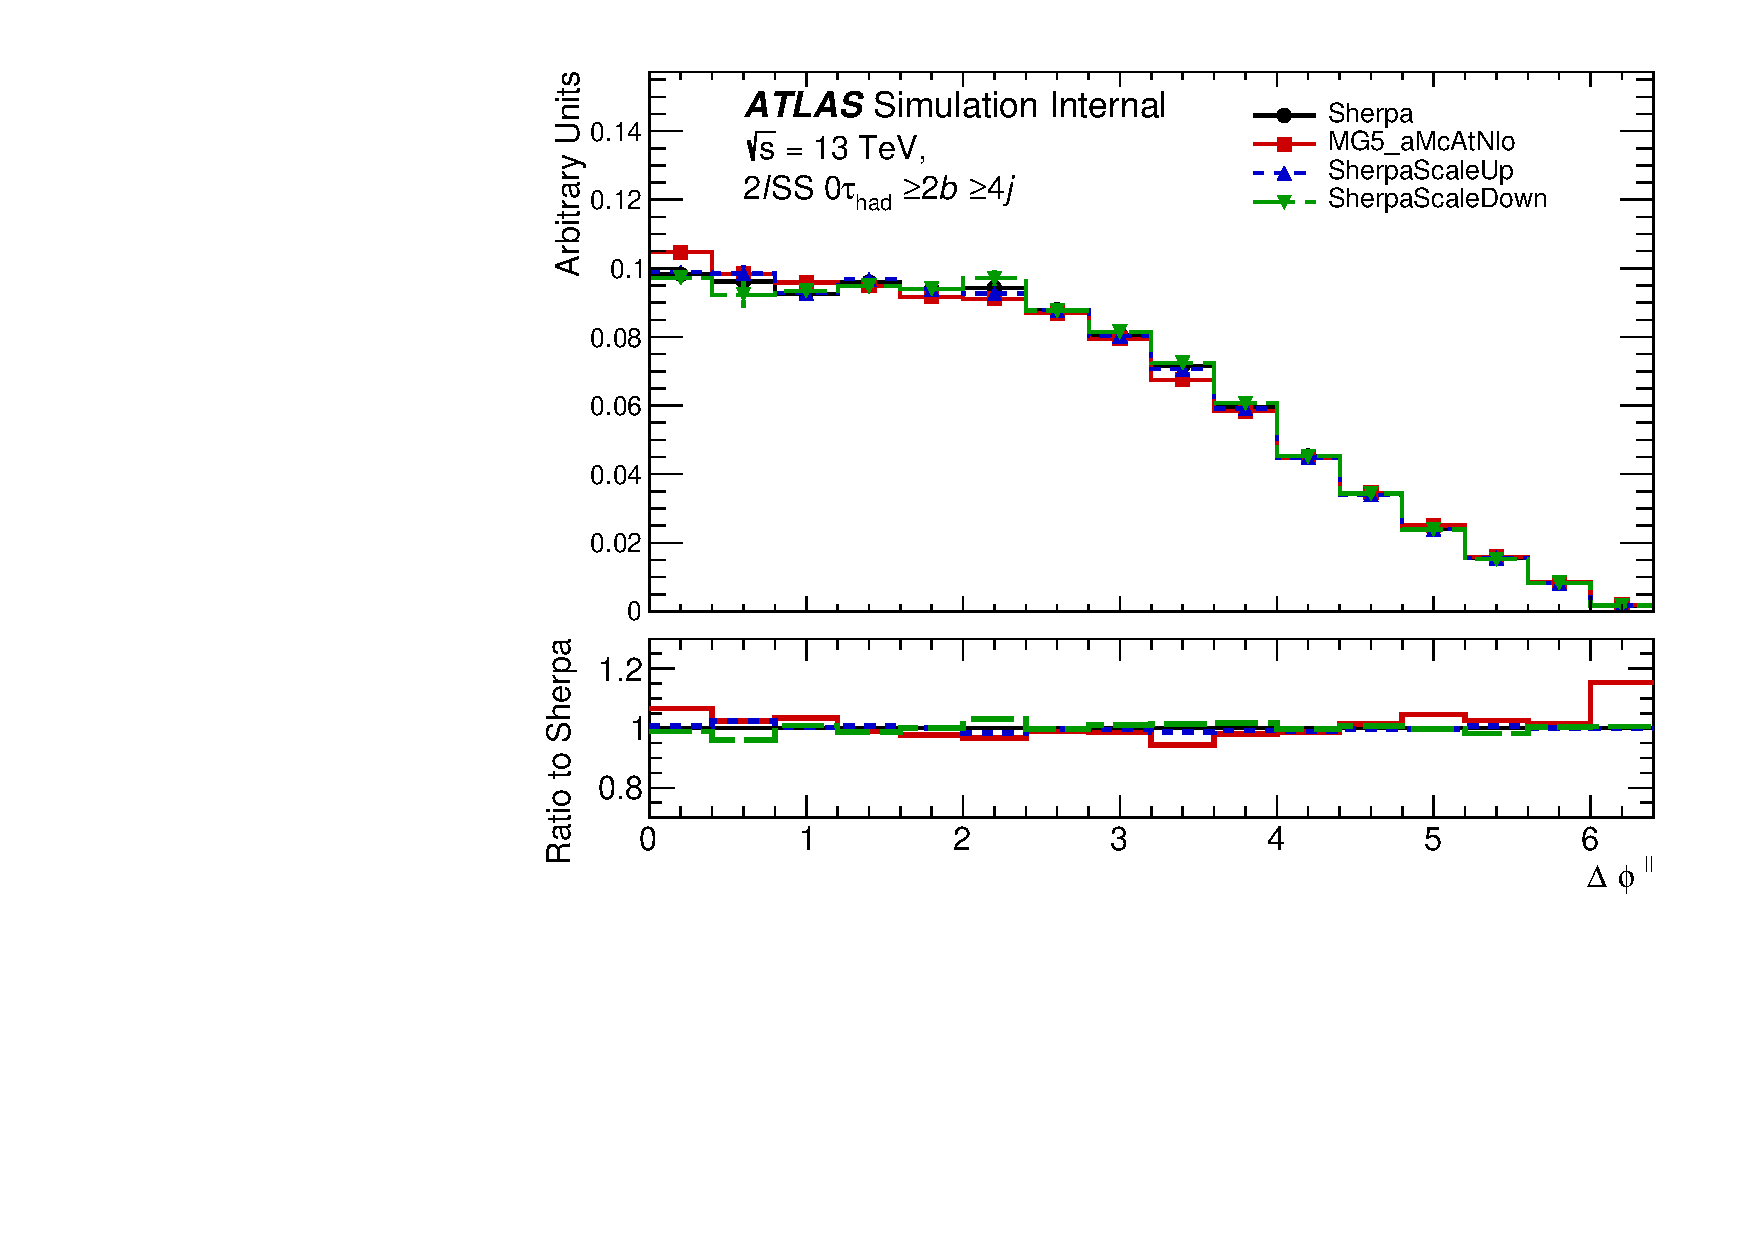
\includegraphics[width=0.45\textwidth]{Plots/ttV/shape/c_Region_1_lep_dPhi} 
  \caption{Distribution of the angular distance between the two leptons (top), maximum between lepton $|\eta_{\ell 0}|$ and $|\eta_{\ell 1}|$ (centre), azimuthal separation between the leptons $\Delta \phi _{\ell \ell }$ (bottom) , for the Region 1 with 1$b$-jet (left) and Region 2 with 2$b$-jets (right) selection requiring four and more jets. Explanation in text.
   \label{ttV:ll_kin}}
\end{figure}
% 



\begin{figure}[!htb]
\centering
	% \hspace{25mm} $DRl_0l_1$  \hspace{20mm} $max|\eta^{\ell\ell}|$\\
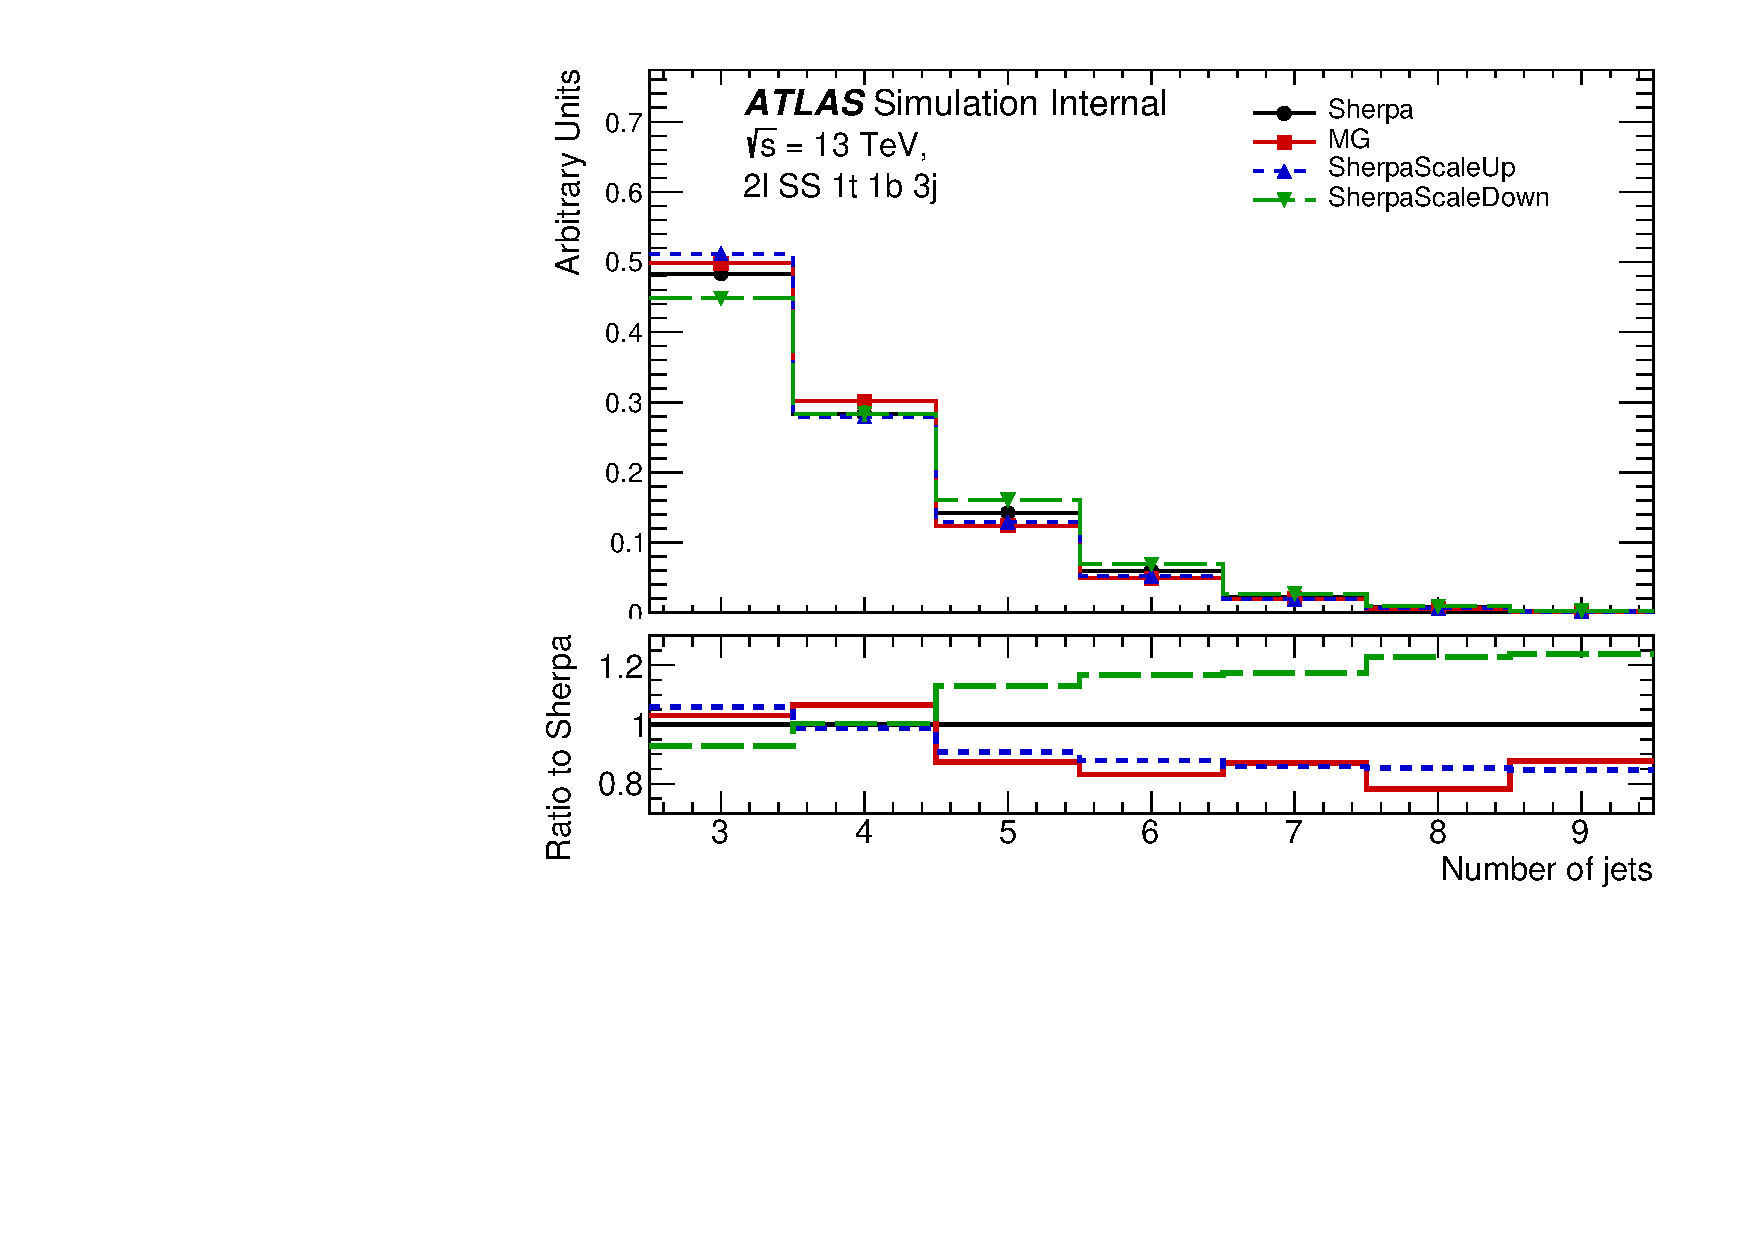
\includegraphics[width=0.45\textwidth]{Plots/ttV/shape/c_Region_4_nJets}
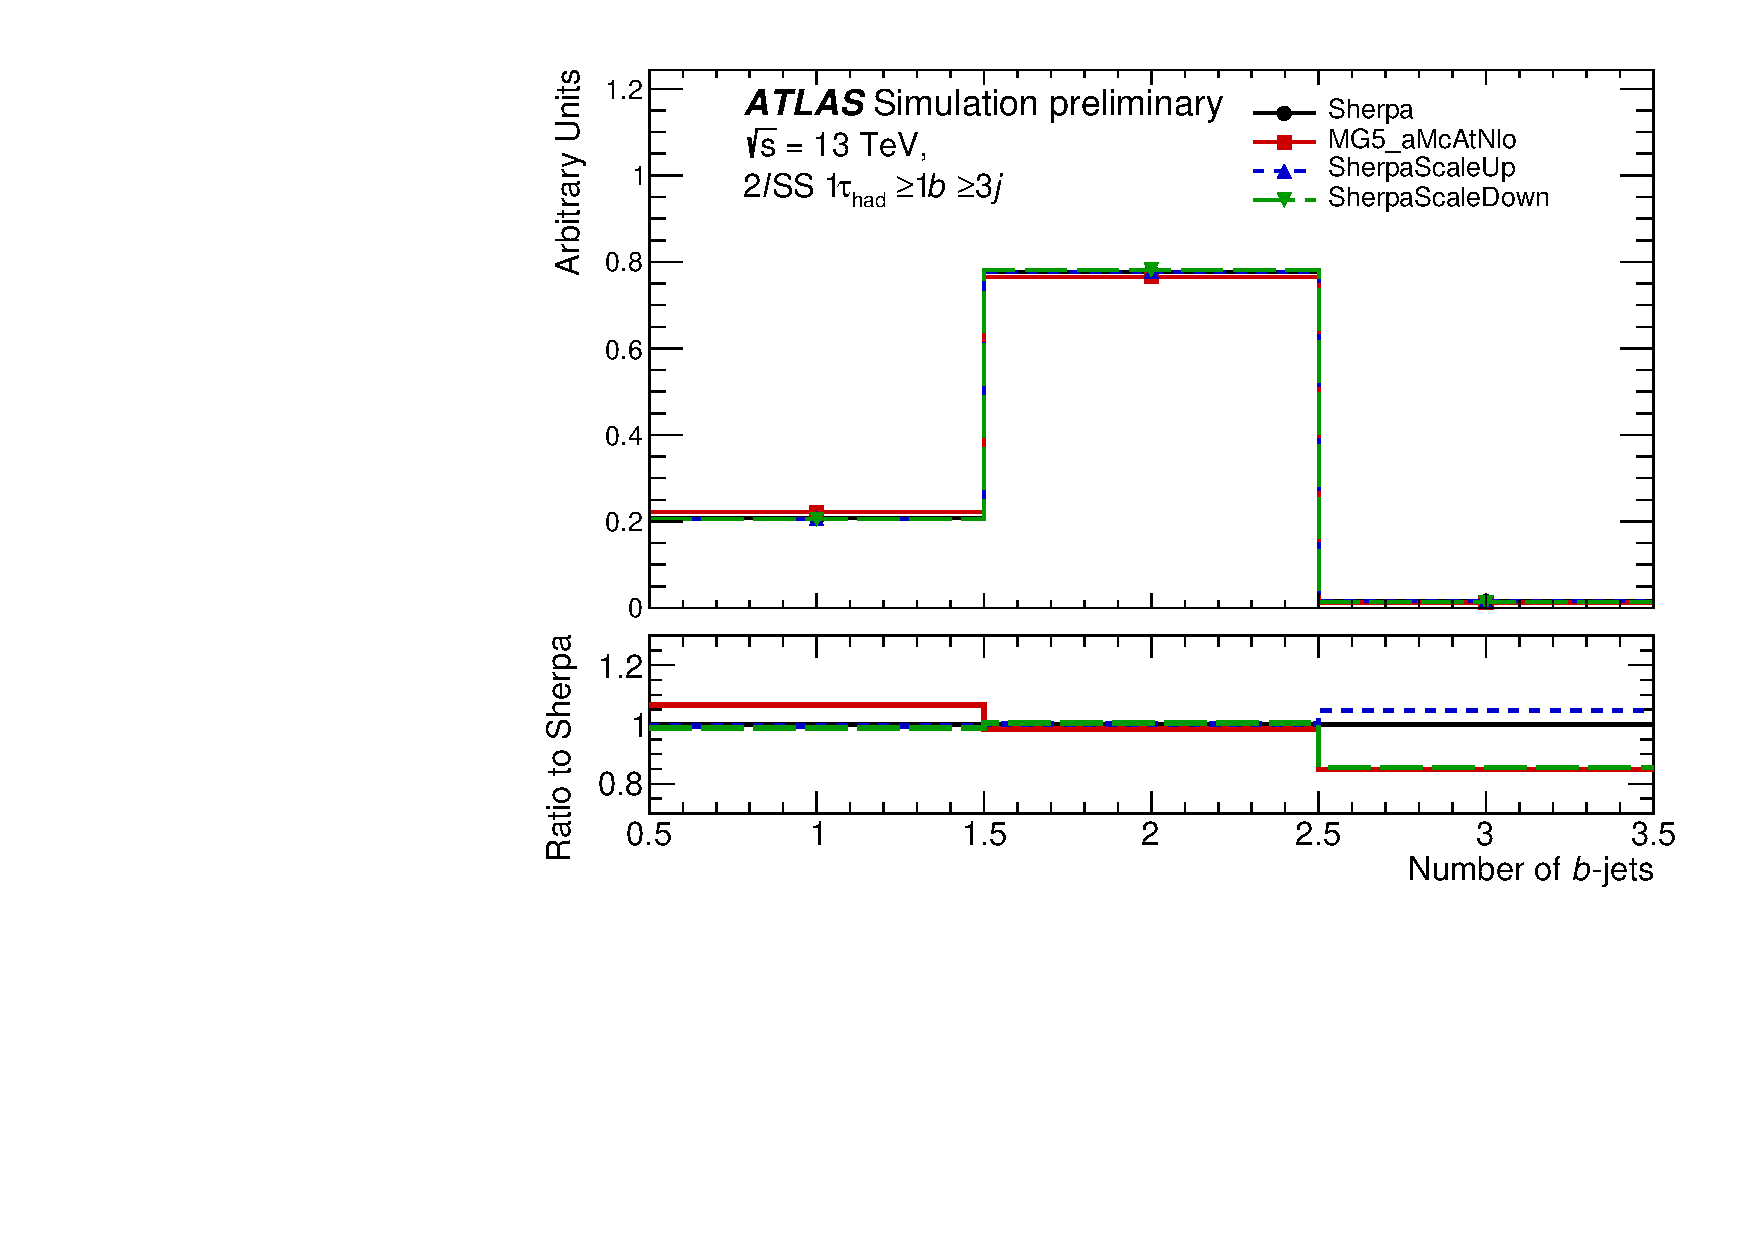
\includegraphics[width=0.45\textwidth]{Plots/ttV/shape/c_Region_4_nBtagJets}\\
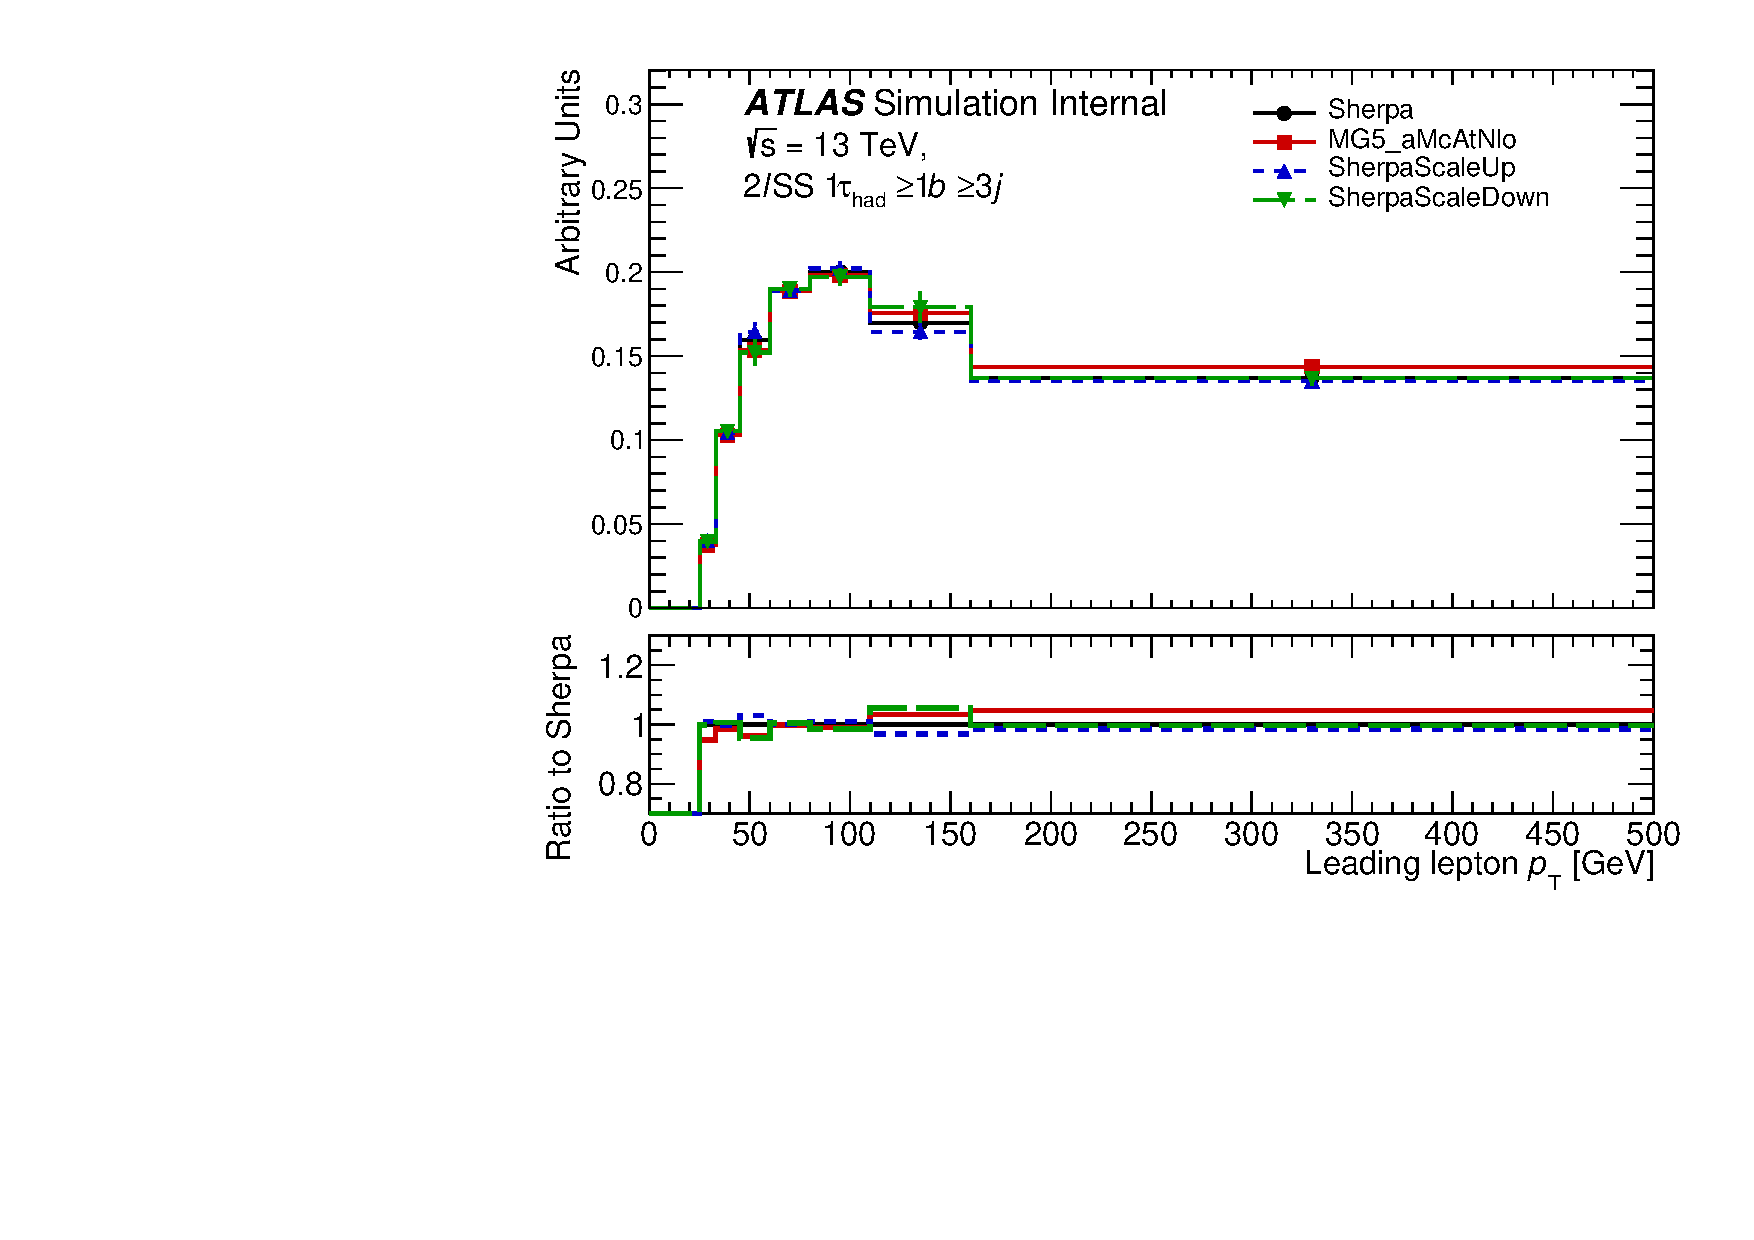
\includegraphics[width=0.45\textwidth]{Plots/ttV/shape/c_Region_4_lep_Pt_0} 
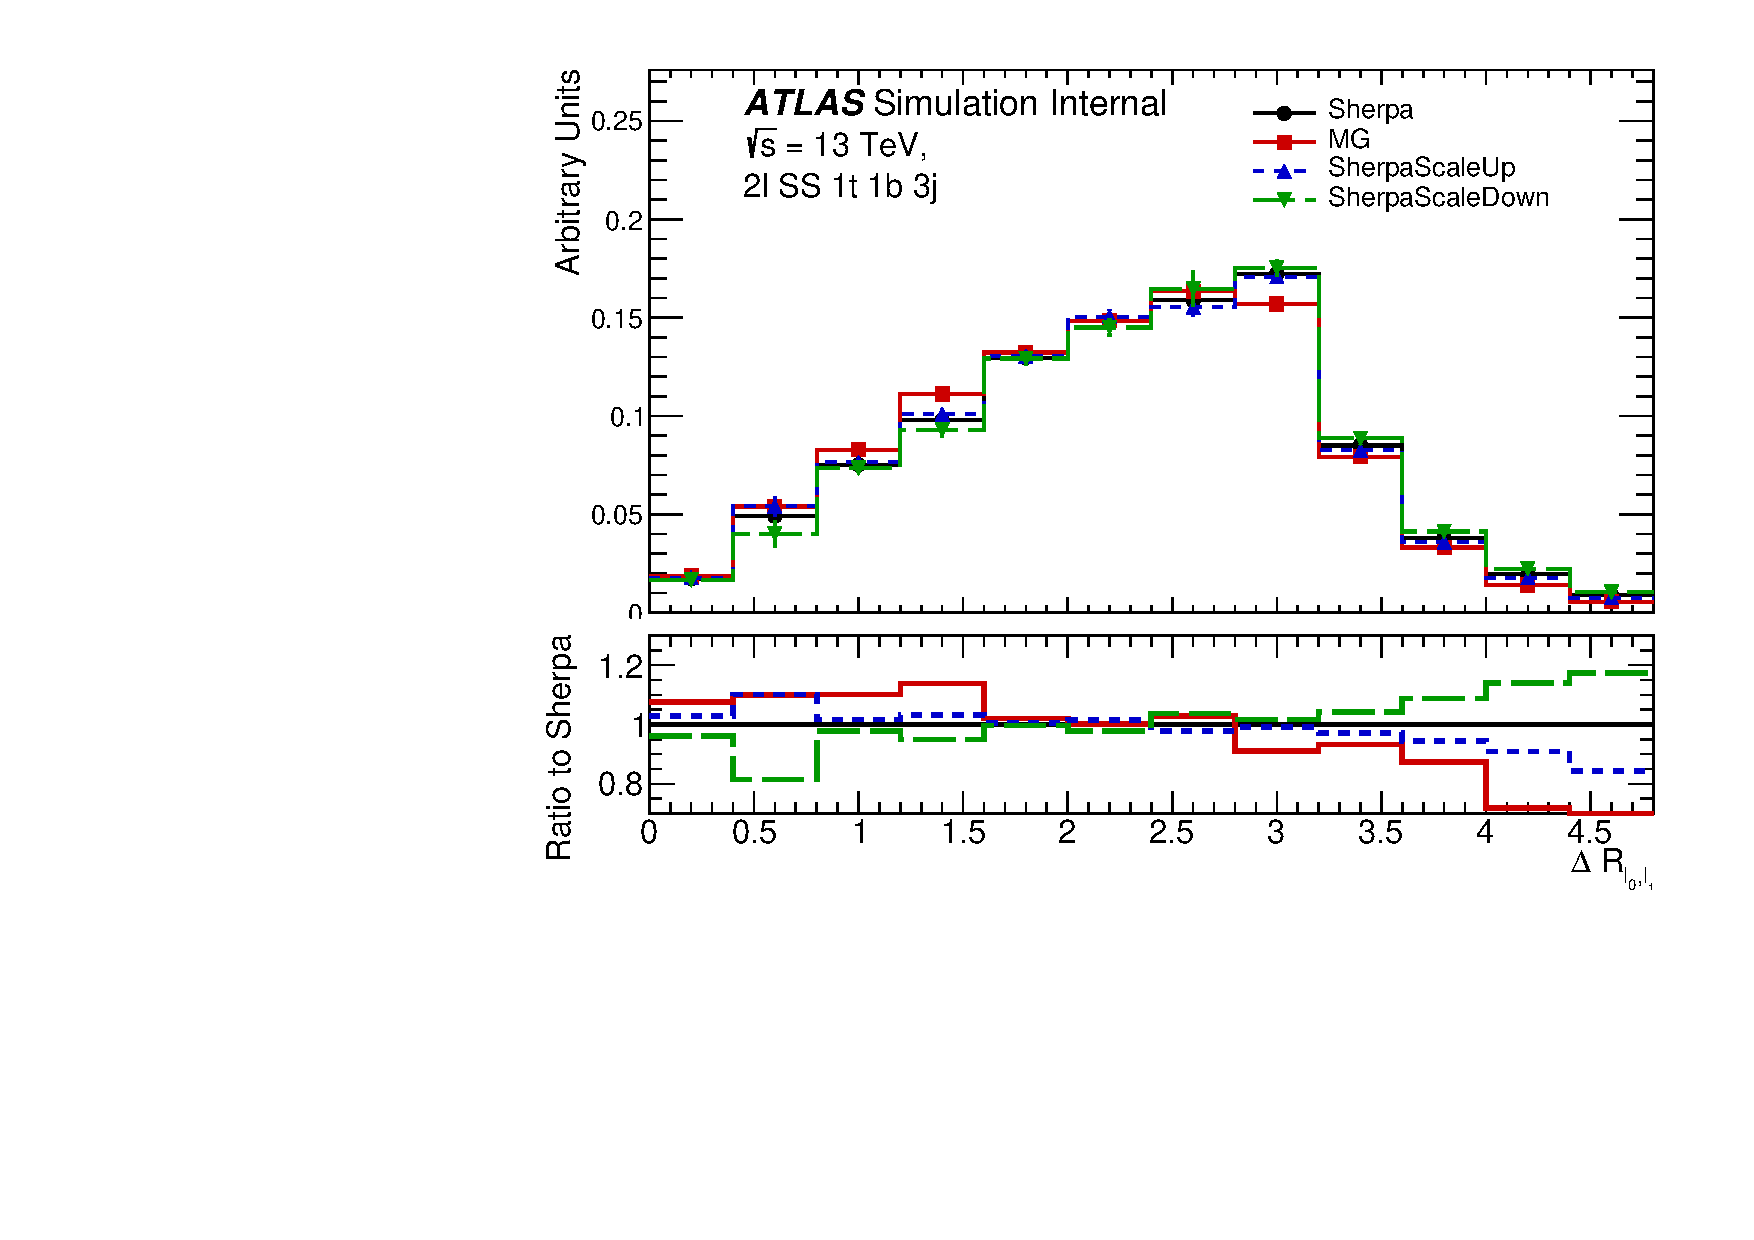
\includegraphics[width=0.45\textwidth]{Plots/ttV/shape/c_Region_4_DRll01}\\
  \caption{Distribution of the the jet multiplicity, number of $b$-jets, the leading lepton transverse momentum and the angular distance between the two leptons  $\Delta R _{\ell \ell }$ for the Region 5 with 1$\tau_{had}$ selection. Explanation in text.
   \label{ttV:tauR_kin}}
\end{figure}
% 



%
%
%
%%
%
%
\subsubsection{Generator comparison}
\label{sec:ttw_gen}

In the following section comparison of the generators will be given in terms of fiducial cross section: 
$\sigma_{fid}^{gen}=A_X^{gen}\times \sigma_{tot}^{gen}$ , where $A_X^{gen}$ is the acceptance factor of particular region, $\sigma_{tot}^{gen}$ is the stotal generator cross section (taken directly from generation - i.e. not including any correction factors), with  $\sigma_{tot}^{Sherpa}=652$fb and  $\sigma_{tot}^{MG}=548$fb for Sherpa and MG correspondingly. The fiducial cross sections of the five regions defined in Section~\ref{sec:ttw_fid} are presented on Figure~\ref{ttV:fid_xs}.
The same set of distribution which was discussed in Section~\ref{sec:ttw_shape} is presented in terms of fiducial cross section in Figures~\ref{ttV:den_4j12b}-\ref{ttV:den_tauR_kin}.

\begin{figure}[!htb]
\centering
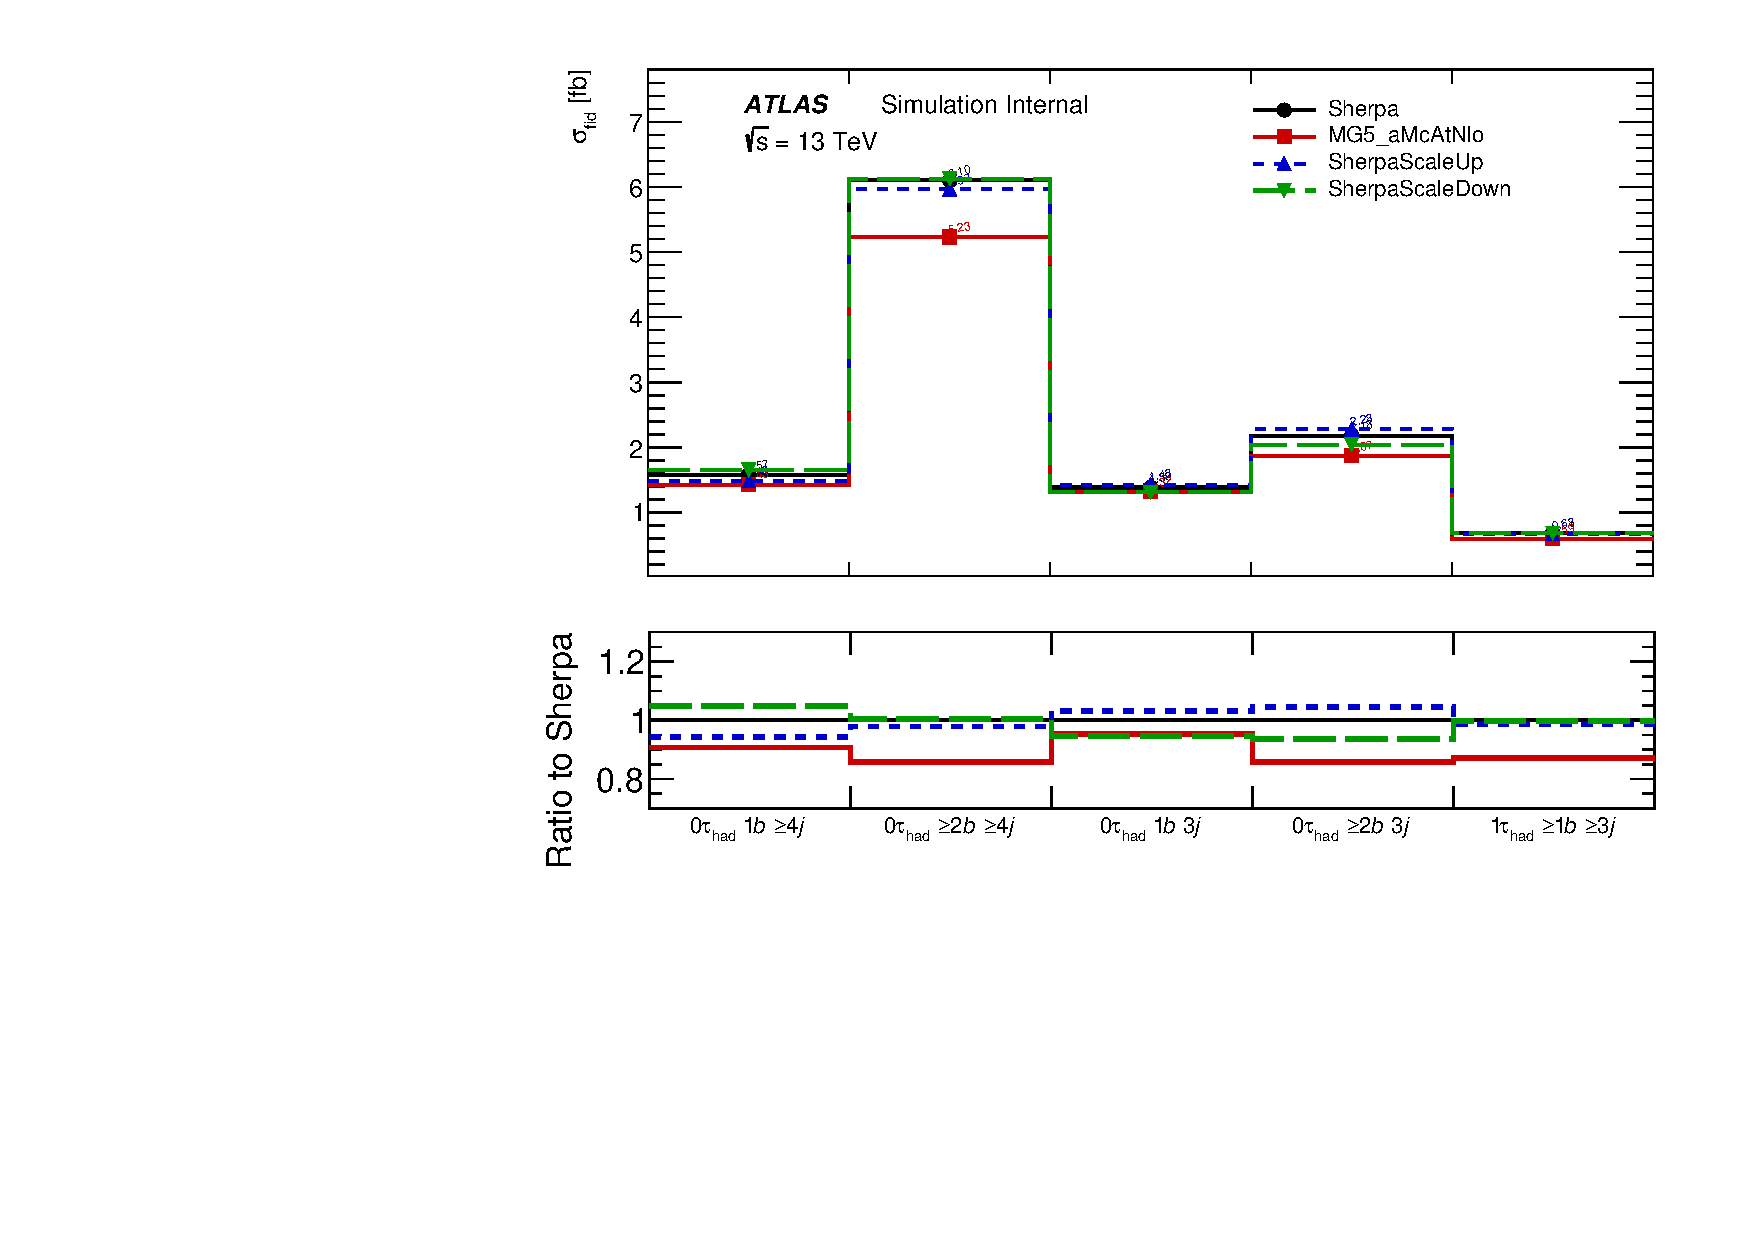
\includegraphics[width=0.45\textwidth]{Plots/ttV/generator/acc_7f}
  \caption{The fiducial cross sections, $\sigma_{fid}^{gen}=A_X^{gen}\times \sigma_{tot}^{gen}$,  of the five regions for $ttW$ analysis. \label{ttV:fid_xs}}
\end{figure}


\begin{figure}[!htb]
\centering
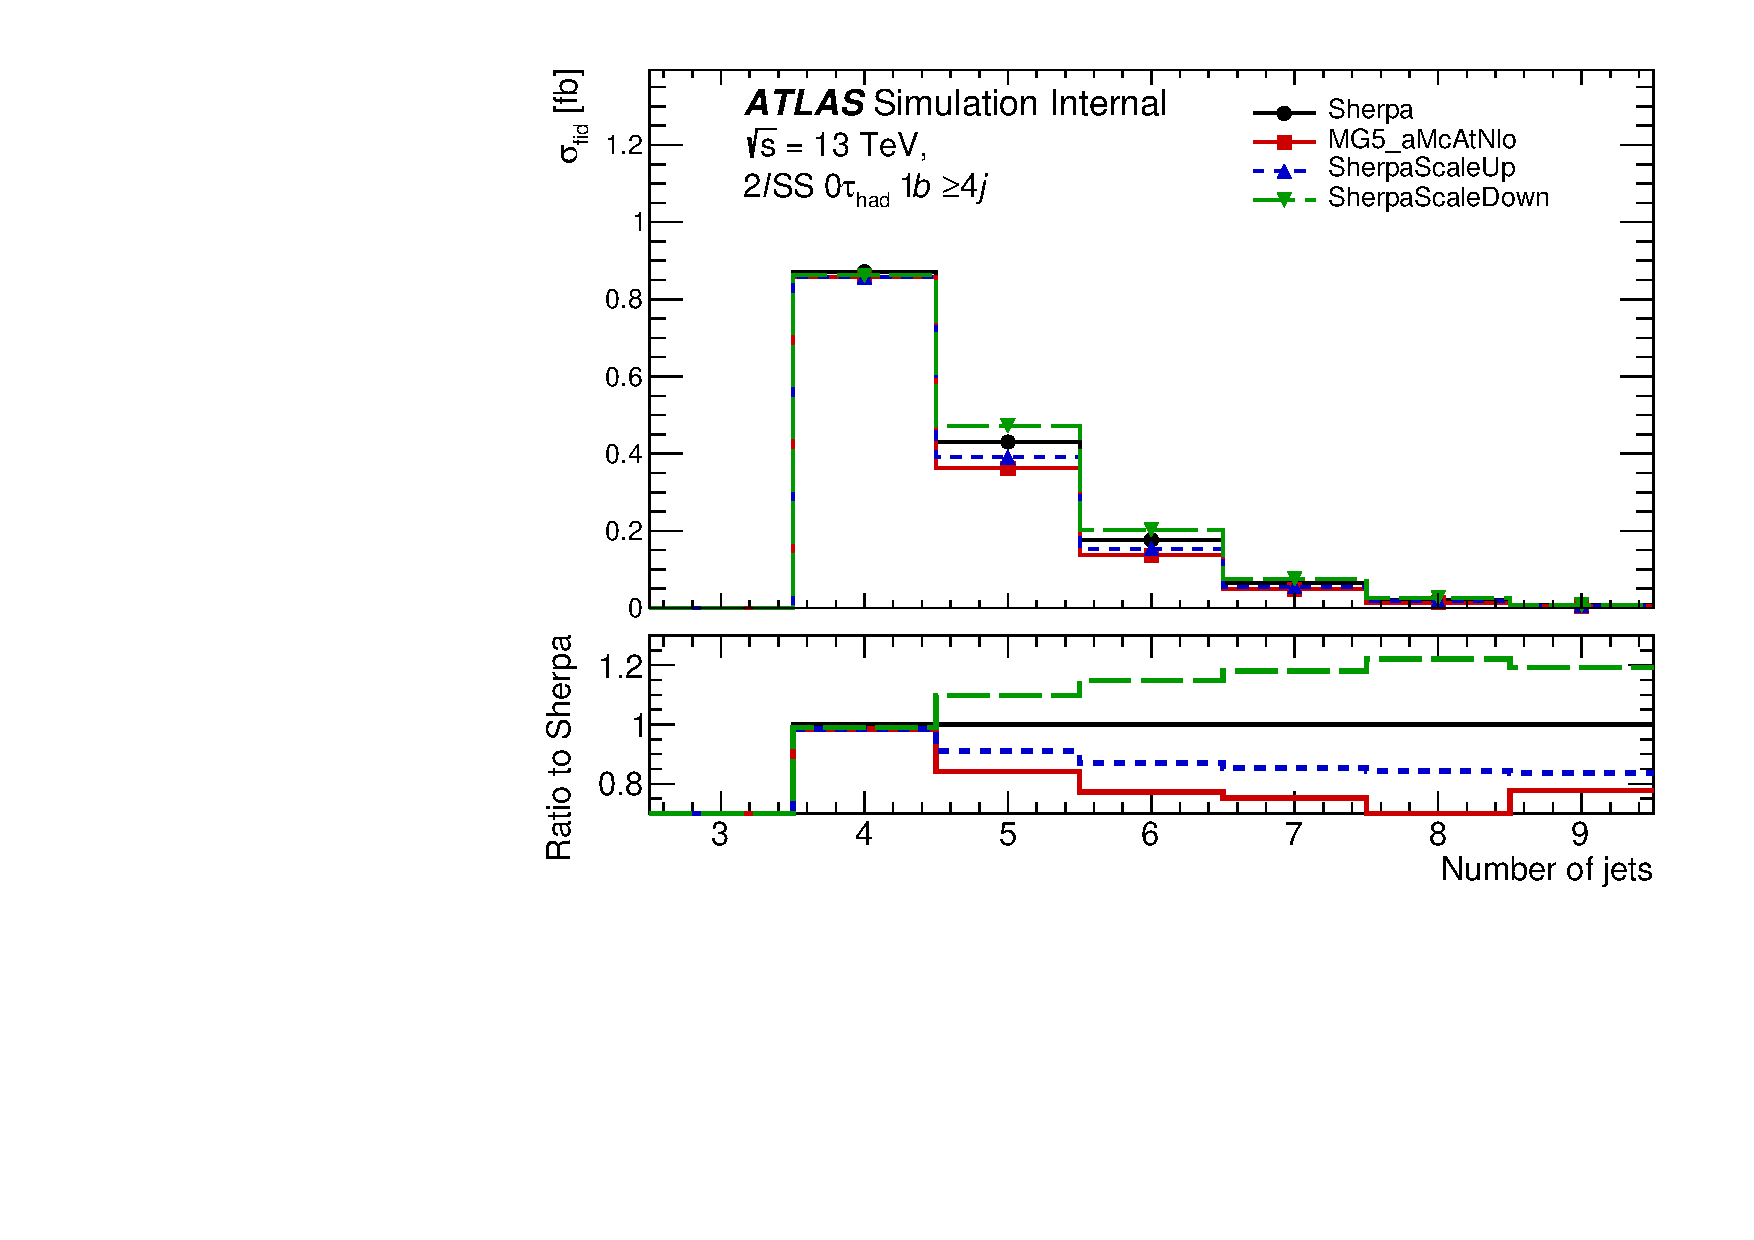
\includegraphics[width=0.45\textwidth]{Plots/ttV/generator/c_Region_0_nJets}
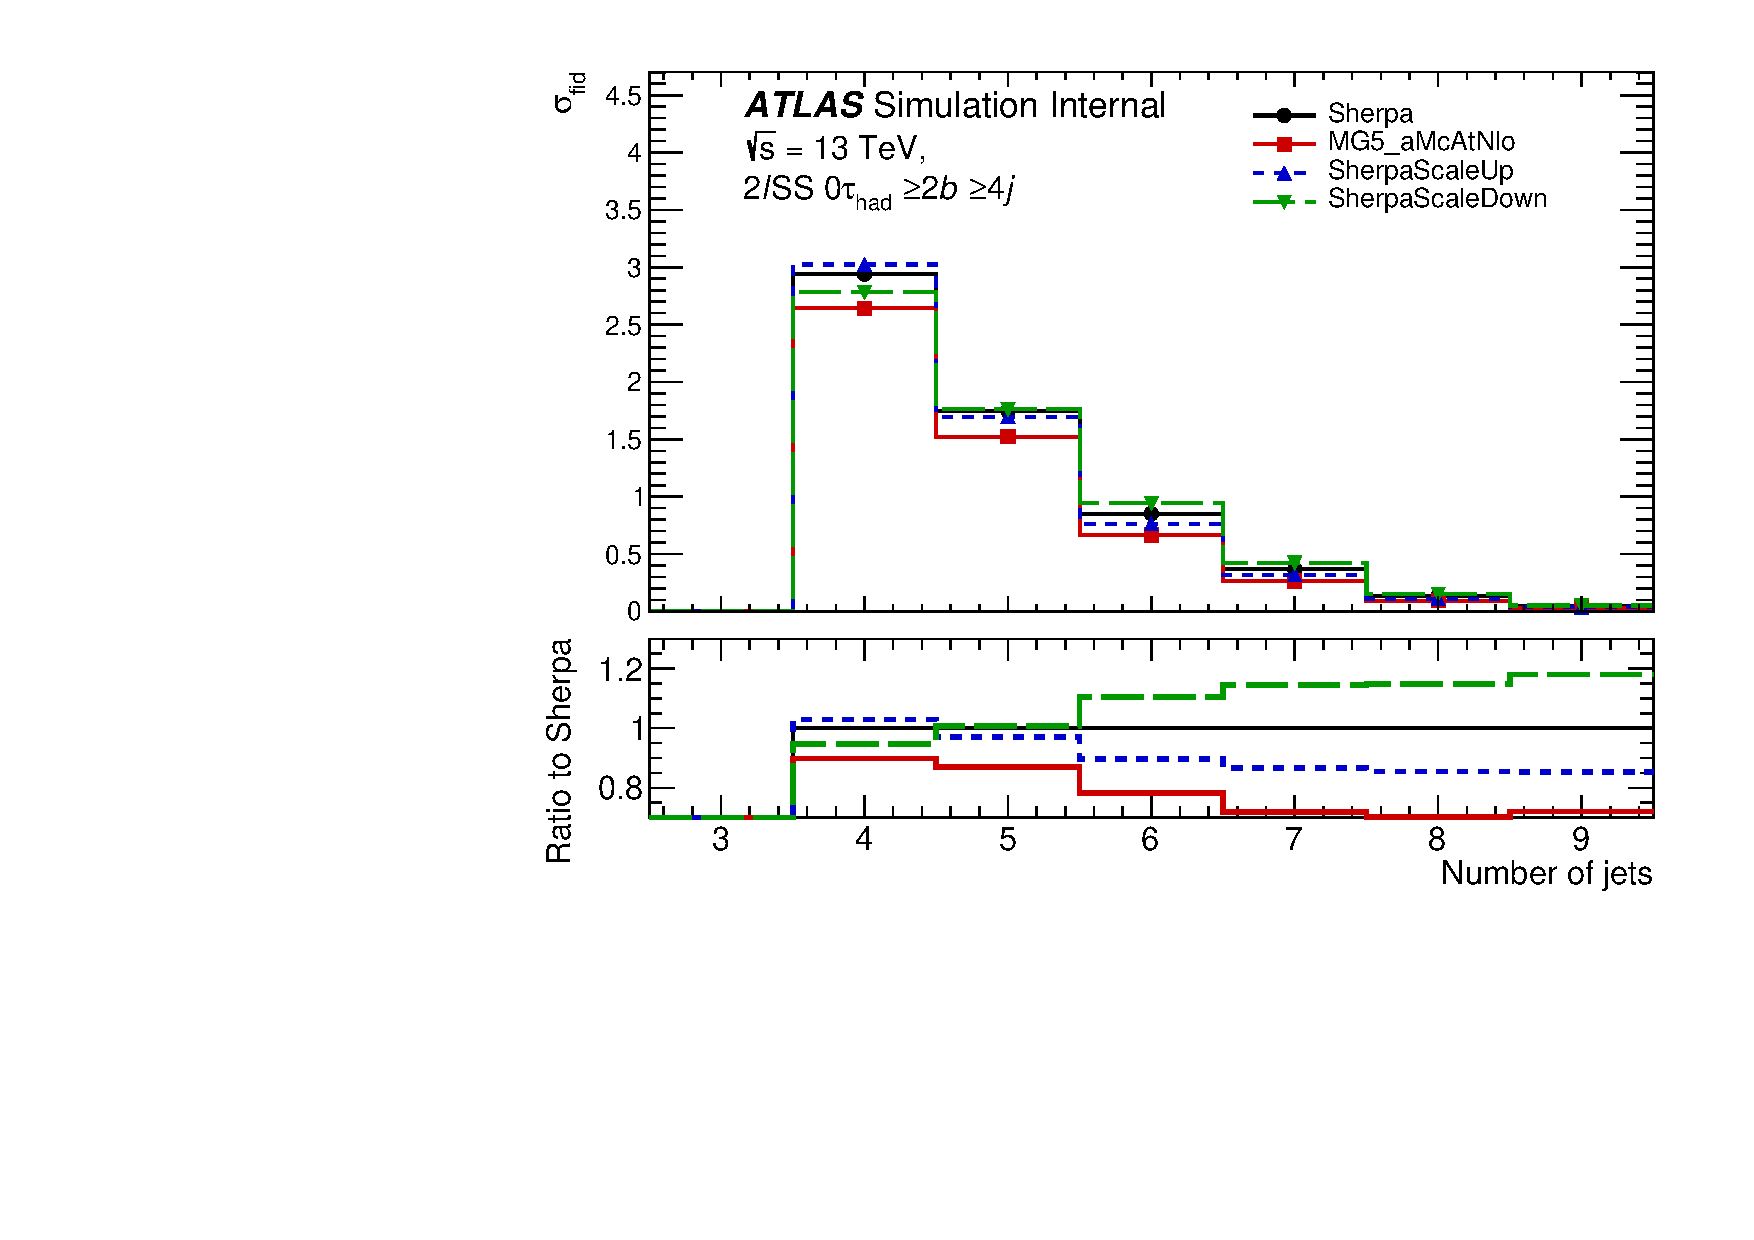
\includegraphics[width=0.45\textwidth]{Plots/ttV/generator/c_Region_1_nJets}\\
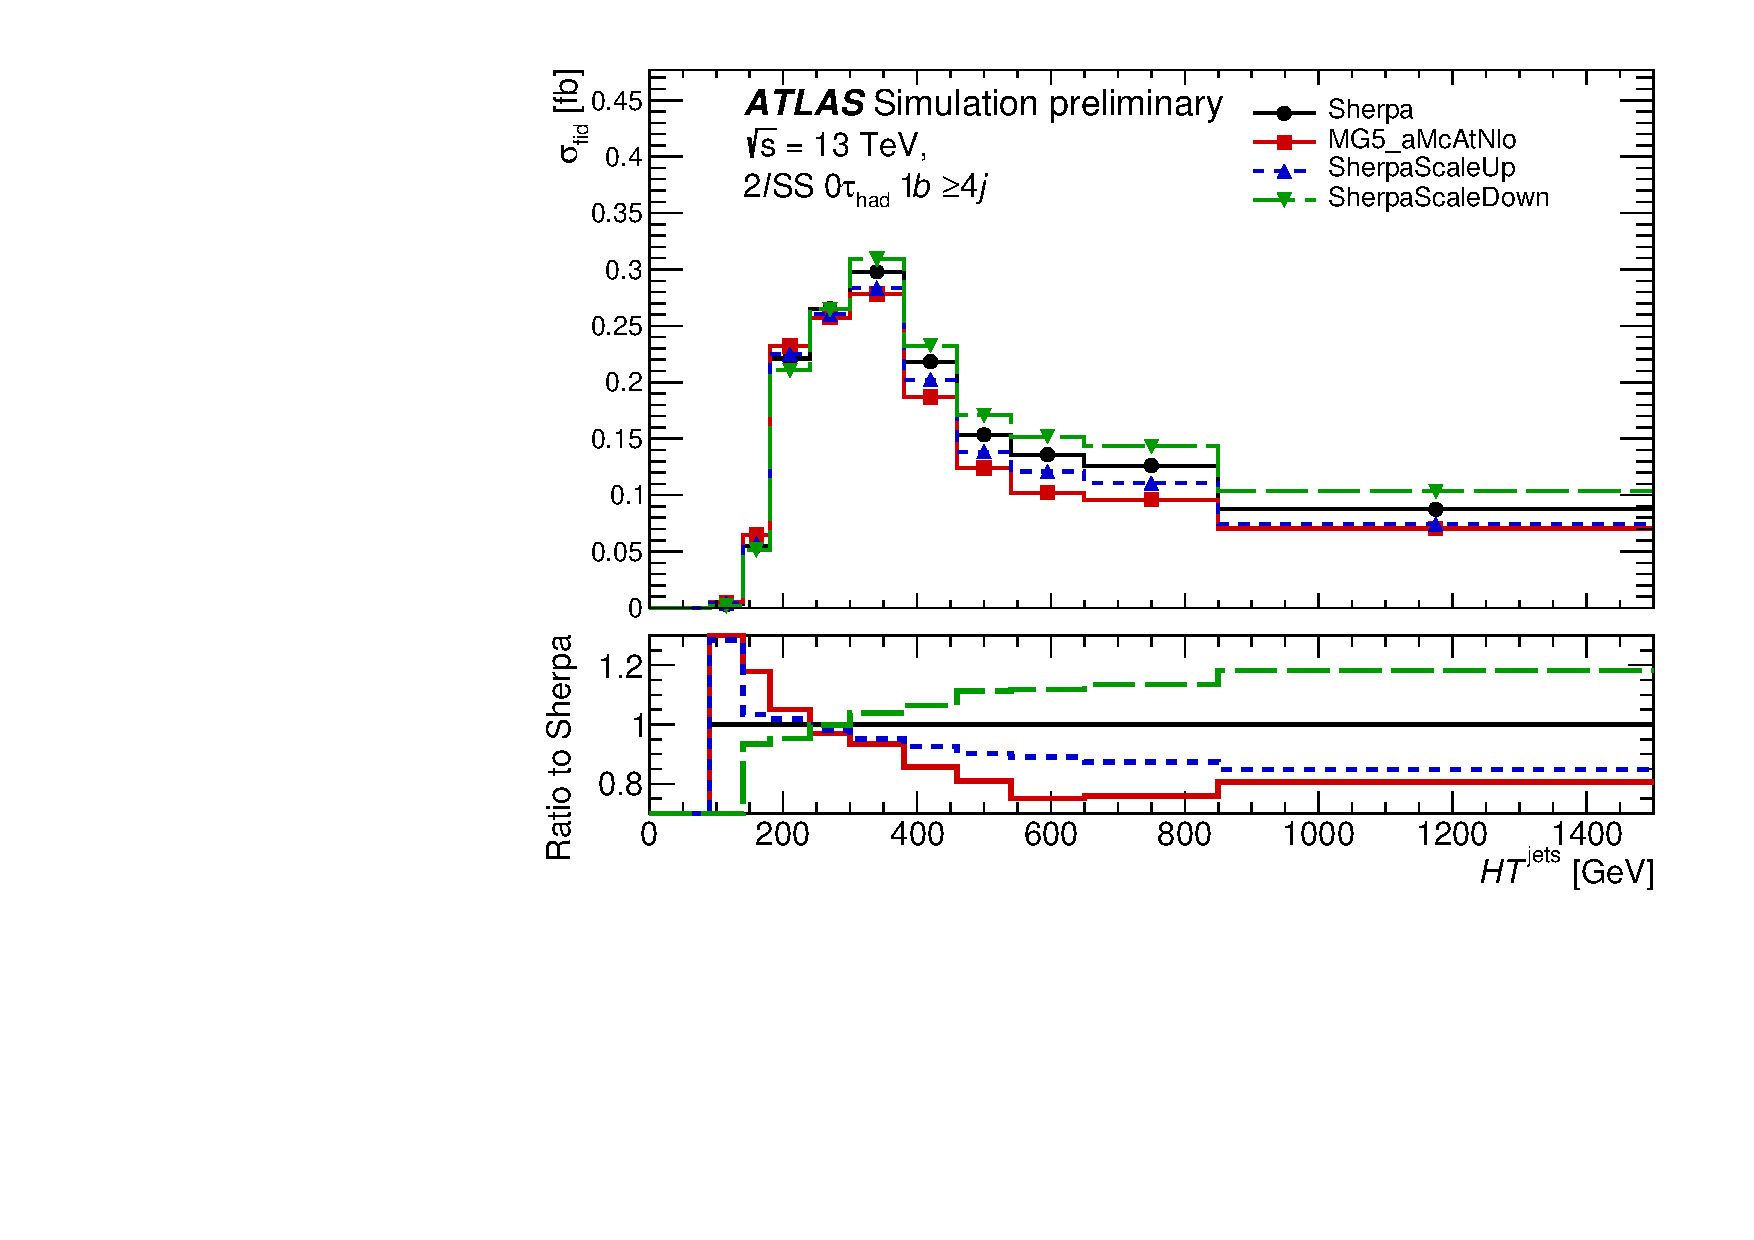
\includegraphics[width=0.45\textwidth]{Plots/ttV/generator/c_Region_0_HT_jets}
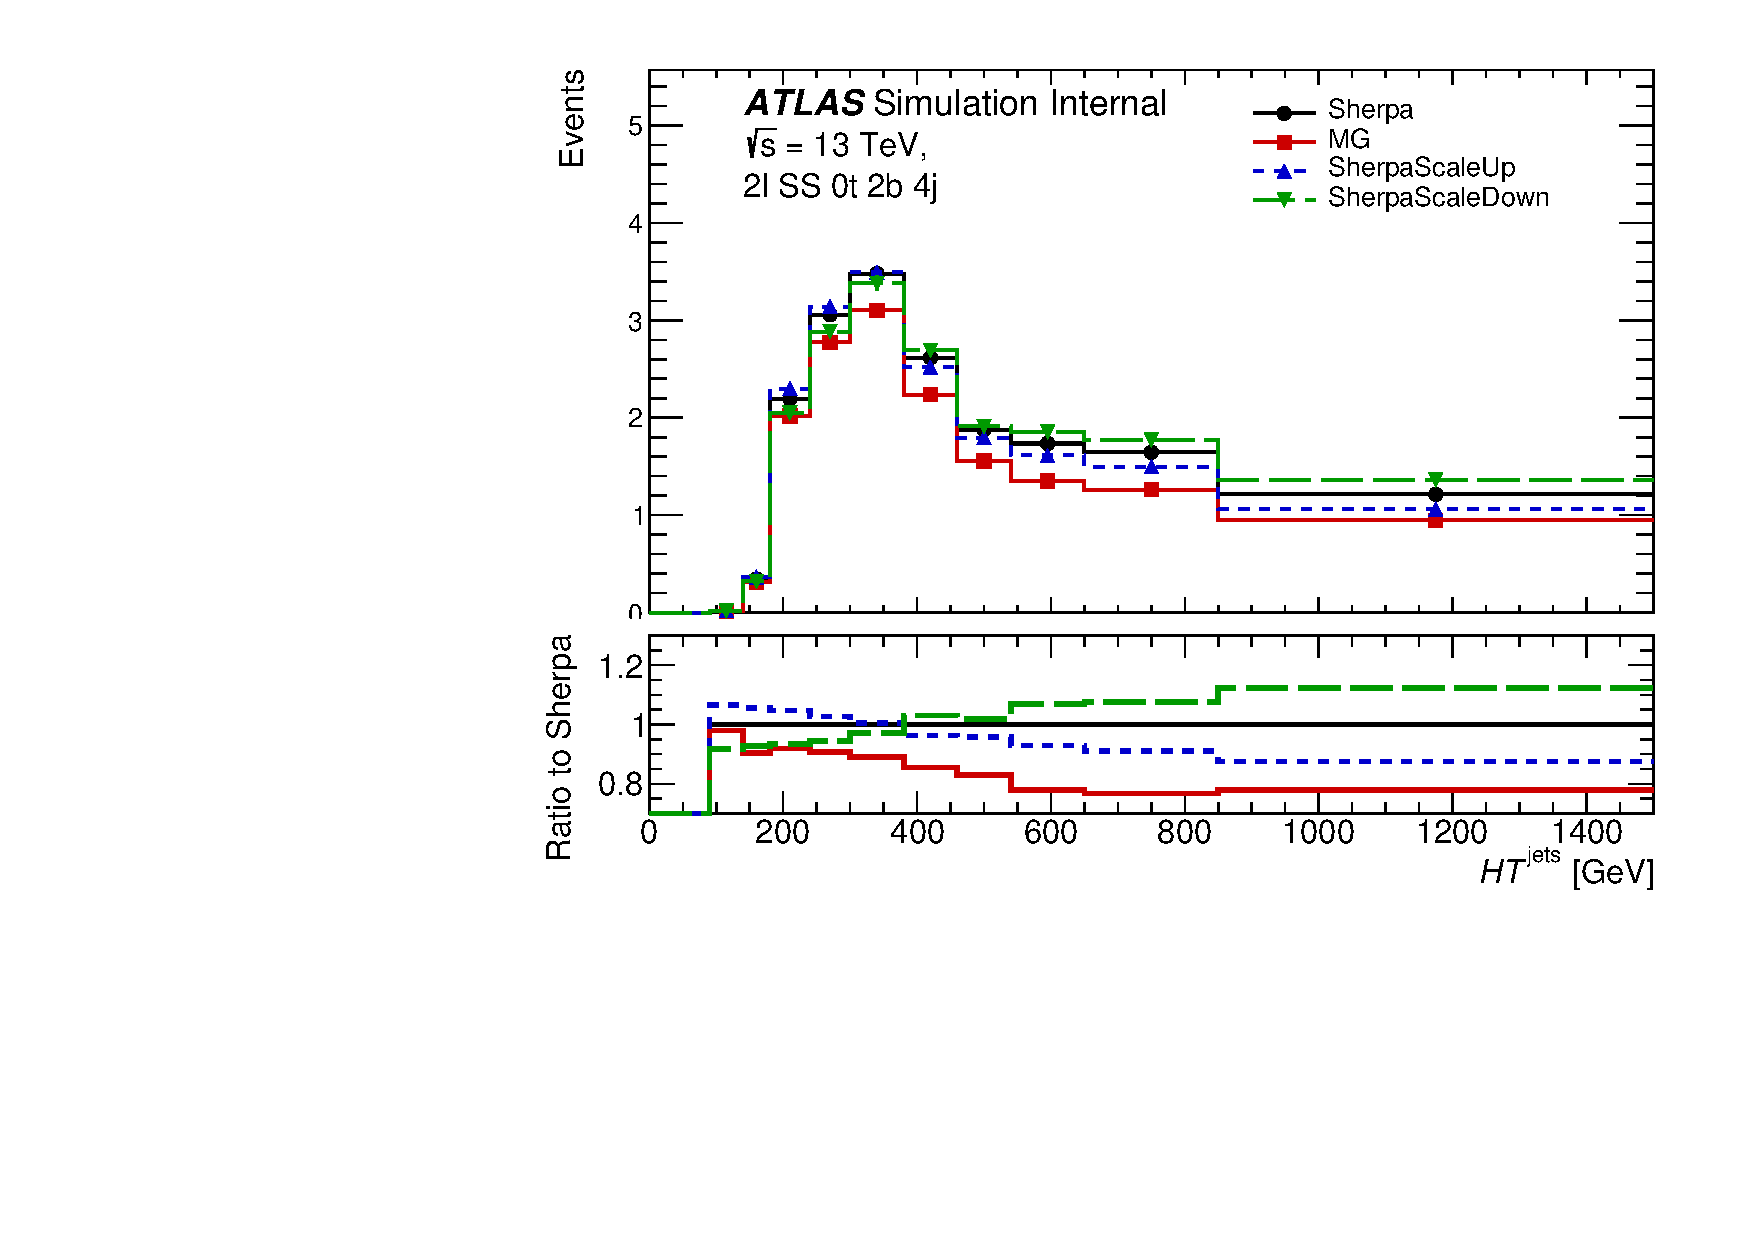
\includegraphics[width=0.45\textwidth]{Plots/ttV/generator/c_Region_1_HT_jets}\\
  \caption{Distribution of the jet multiplicities (top) and the sum of jets transverse momentum, $HT^{\text{jets}}$ (bottom), for the Region 1 with 1$b$-jet (left) and Region 2 with 2$b$-jets (right) selection requiring four and more jets. Explanation in text. \label{ttV:den_4j12b}}
\end{figure}


\begin{figure}[!htb]
\centering
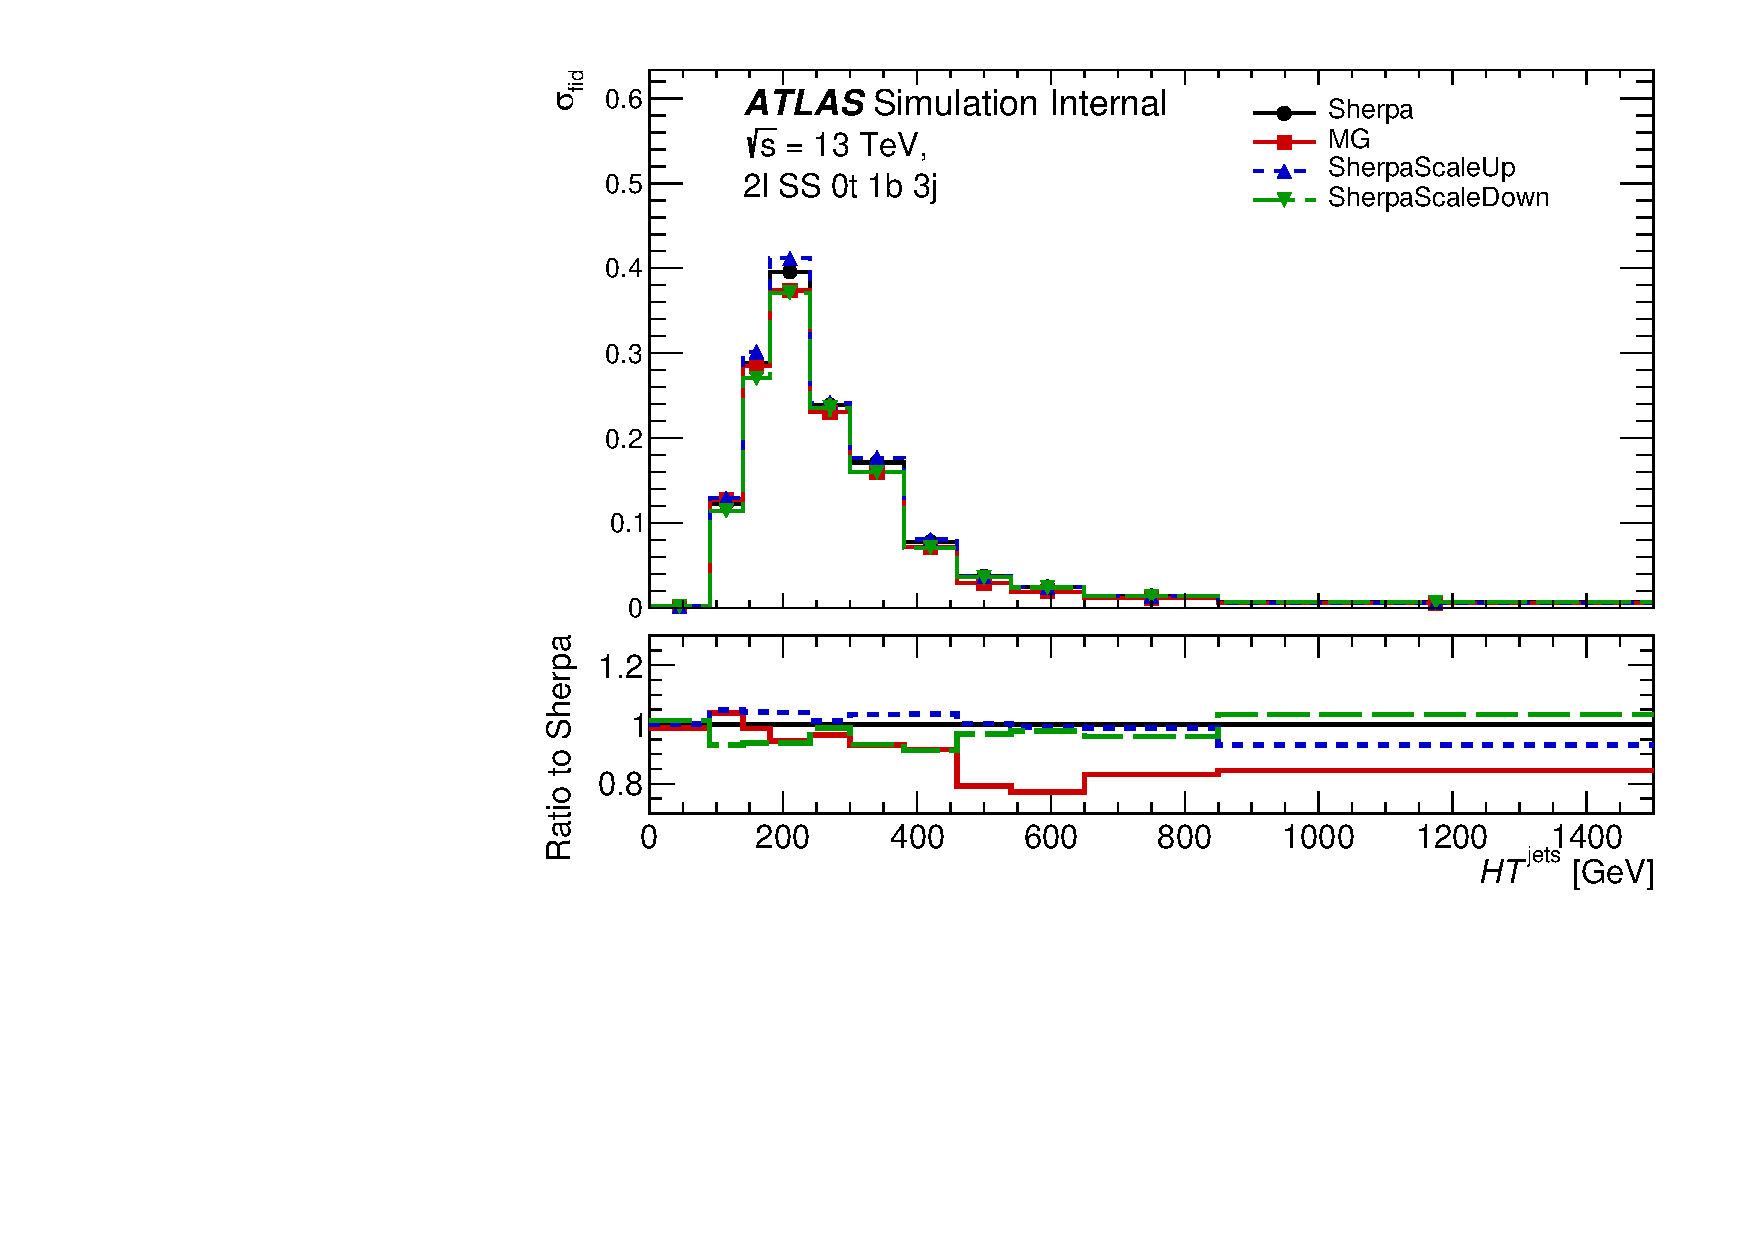
\includegraphics[width=0.45\textwidth]{Plots/ttV/generator/c_Region_2_HT_jets}
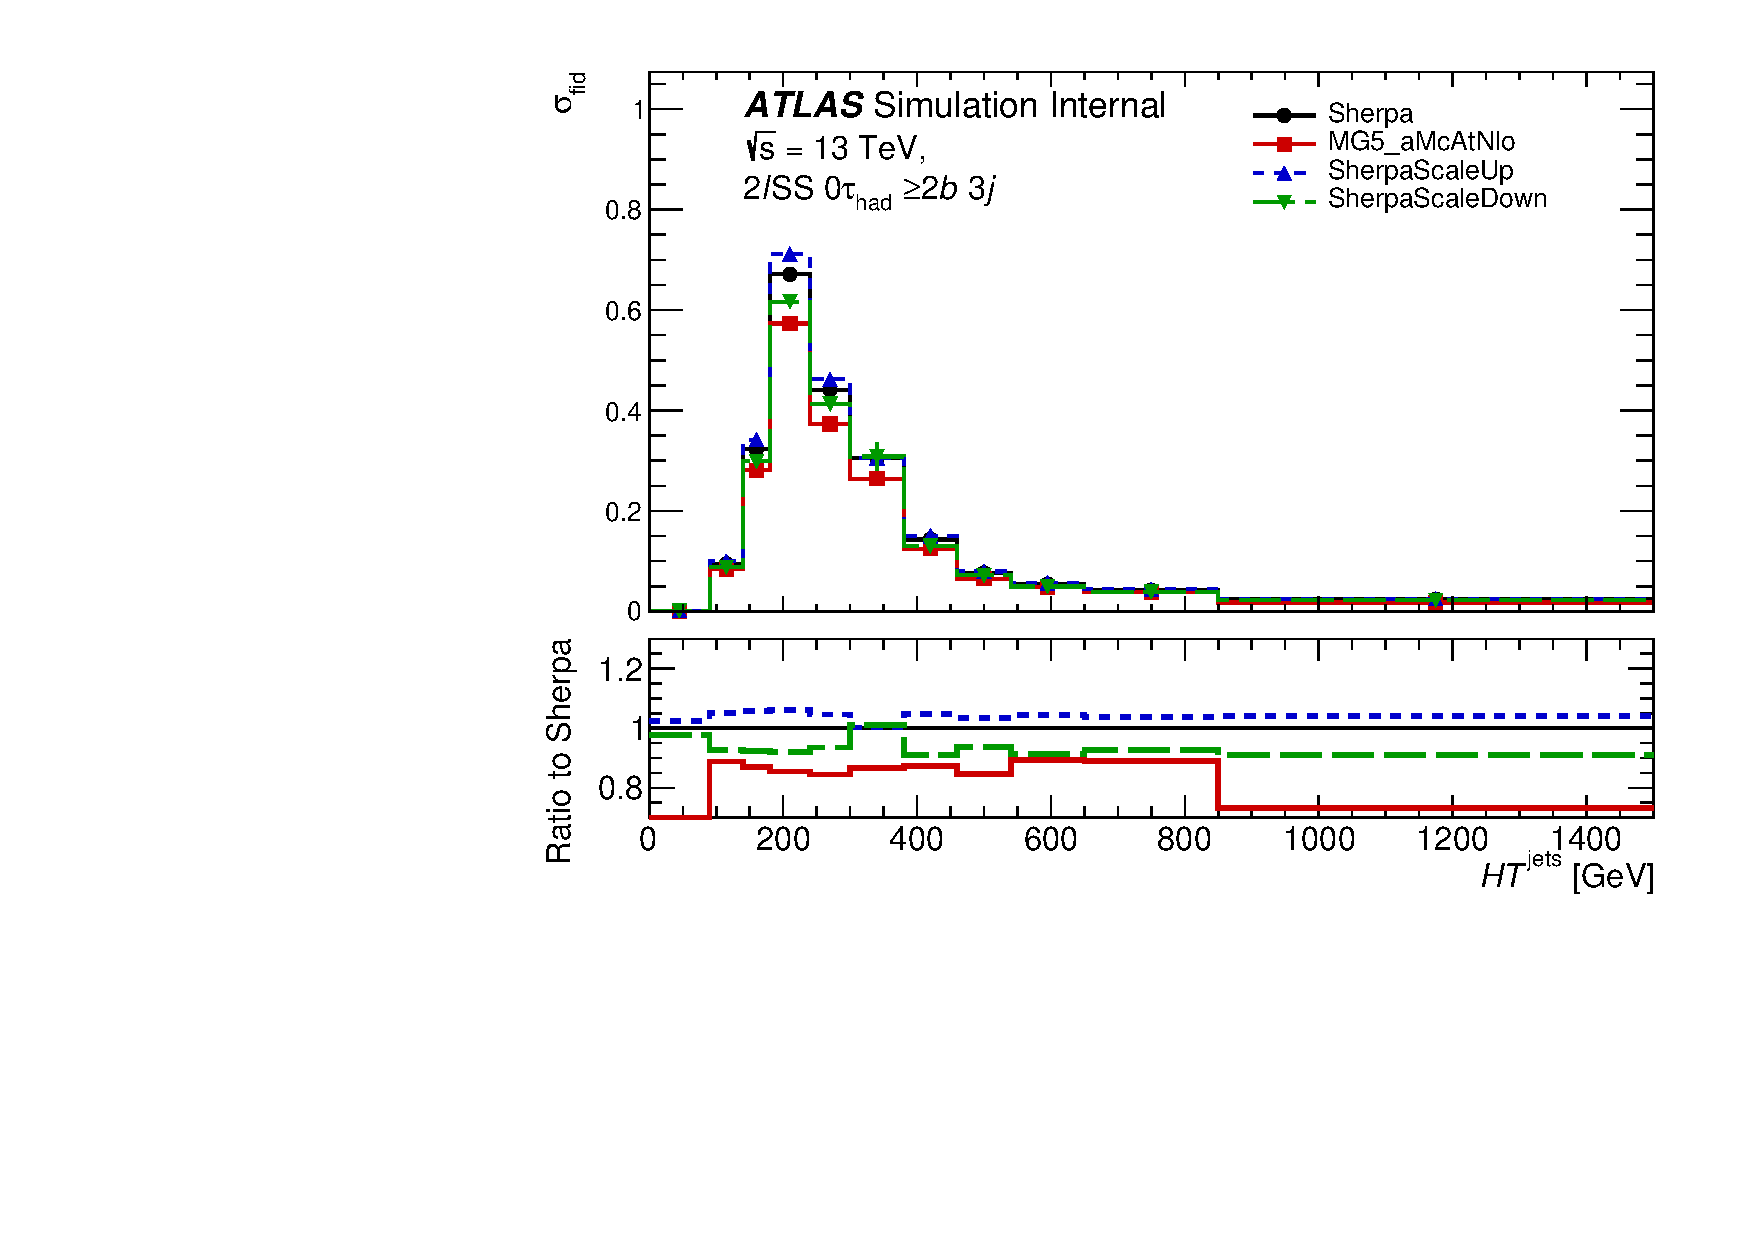
\includegraphics[width=0.45\textwidth]{Plots/ttV/generator/c_Region_3_HT_jets}\\
  \caption{Distribution of the sum of jets transverse momentum, $HT^{\text{jets}}$, for the Region 3 with 1$b$-jet (left) and Region 4 with 2$b$-jets (right) selection requiring exactly three jets. Explanation in text. \label{ttV:den_3j12b}}
\end{figure}


\begin{figure}[!htb]
\centering
\includegraphics[width=0.45\textwidth]{Plots/ttV/generator/c_Region_0_nBtagJets}
\includegraphics[width=0.45\textwidth]{Plots/ttV/generator/c_Region_1_nBtagJets}\\
\includegraphics[width=0.45\textwidth]{Plots/ttV/generator/c_Region_0_Bjet_Pt_0}
\includegraphics[width=0.45\textwidth]{Plots/ttV/generator/c_Region_1_Bjet_Pt_0}\\
  \caption{Distribution of the $b$-jet multiplicities (top) and the leading $b$-jet transverse momentum (bottom), for the Region 1 with 1$b$-jet (left) and Region 2 with 2$b$-jets (right) selection requiring four and more jets. Explanation in text. \label{ttV:den_4jbinfo}}
\end{figure}



\begin{figure}[!htb]
\centering
\includegraphics[width=0.45\textwidth]{Plots/ttV/generator/c_Region_0_lep_Pt_0}
\includegraphics[width=0.45\textwidth]{Plots/ttV/generator/c_Region_1_lep_Pt_0}\\
%\includegraphics[width=0.45\textwidth]{Plots/ttV/generator/c_Region_1_lep_Pt_1}
\includegraphics[width=0.45\textwidth]{Plots/ttV/generator/c_Region_0_min_DRl0j}
\includegraphics[width=0.45\textwidth]{Plots/ttV/generator/c_Region_1_min_DRl0j}\\
  \caption{Distribution of the leading lepton transverse momentum (top) and the minimum angular separation between the leading lepton and the nearest jet (bottom), for the Region 1 with 1$b$-jet (left) and Region 2 with 2$b$-jets (right) selection requiring four and more jets. Explanation in text.
  \label{ttV:den_lep_kin}}
\end{figure}

\begin{figure}[!htb]
\centering
	% \hspace{25mm} $DRl_0l_1$  \hspace{20mm} $max|\eta^{\ell\ell}|$\\
\includegraphics[width=0.45\textwidth]{Plots/ttV/generator/c_Region_0_DRll01}
\includegraphics[width=0.45\textwidth]{Plots/ttV/generator/c_Region_1_DRll01}\\
\includegraphics[width=0.45\textwidth]{Plots/ttV/generator/c_Region_0_maxEta_ll} 
\includegraphics[width=0.45\textwidth]{Plots/ttV/generator/c_Region_1_maxEta_ll}\\
\includegraphics[width=0.45\textwidth]{Plots/ttV/generator/c_Region_0_lep_dPhi} 
\includegraphics[width=0.45\textwidth]{Plots/ttV/generator/c_Region_1_lep_dPhi} 
  \caption{Distribution of the angular distance between the two leptons (top), maximum between lepton $|\eta_{\ell 0}|$ and $|\eta_{\ell 1}|$ (centre), azimuthal separation between the leptons $\Delta \phi _{\ell \ell }$ (bottom) , for the Region 1 with 1$b$-jet (left) and Region 2 with 2$b$-jets (right) selection requiring four and more jets. Explanation in text.
   \label{ttV:den_ll_kin}}
\end{figure}
% 



\begin{figure}[!htb]
\centering
	% \hspace{25mm} $DRl_0l_1$  \hspace{20mm} $max|\eta^{\ell\ell}|$\\
\includegraphics[width=0.45\textwidth]{Plots/ttV/generator/c_Region_4_nJets}
\includegraphics[width=0.45\textwidth]{Plots/ttV/generator/c_Region_4_nBtagJets}\\
\includegraphics[width=0.45\textwidth]{Plots/ttV/generator/c_Region_4_lep_Pt_0} 
\includegraphics[width=0.45\textwidth]{Plots/ttV/generator/c_Region_4_DRll01}\\
  \caption{Distribution of the the jet multiplicity, number of $b$-jets, the leading lepton transverse momentum and the angular distance between the two leptons  $\Delta R _{\ell \ell }$ for the Region 5 with 1$\tau_{had}$ selection. Explanation in text.
   \label{ttV:den_tauR_kin}}
\end{figure}
% 


%-------------------------------------------------------------------------------
\section*{Acknowledgements}
%-------------------------------------------------------------------------------

%% Acknowledgements for papers with collision data
% Version 24-Oct-2018

% Standard acknowledgements start here
%----------------------------------------------
We thank CERN for the very successful operation of the LHC, as well as the
support staff from our institutions without whom ATLAS could not be
operated efficiently.

We acknowledge the support of ANPCyT, Argentina; YerPhI, Armenia; ARC, Australia; BMWFW and FWF, Austria; ANAS, Azerbaijan; SSTC, Belarus; CNPq and FAPESP, Brazil; NSERC, NRC and CFI, Canada; CERN; CONICYT, Chile; CAS, MOST and NSFC, China; COLCIENCIAS, Colombia; MSMT CR, MPO CR and VSC CR, Czech Republic; DNRF and DNSRC, Denmark; IN2P3-CNRS, CEA-DRF/IRFU, France; SRNSFG, Georgia; BMBF, HGF, and MPG, Germany; GSRT, Greece; RGC, Hong Kong SAR, China; ISF and Benoziyo Center, Israel; INFN, Italy; MEXT and JSPS, Japan; CNRST, Morocco; NWO, Netherlands; RCN, Norway; MNiSW and NCN, Poland; FCT, Portugal; MNE/IFA, Romania; MES of Russia and NRC KI, Russian Federation; JINR; MESTD, Serbia; MSSR, Slovakia; ARRS and MIZ\v{S}, Slovenia; DST/NRF, South Africa; MINECO, Spain; SRC and Wallenberg Foundation, Sweden; SERI, SNSF and Cantons of Bern and Geneva, Switzerland; MOST, Taiwan; TAEK, Turkey; STFC, United Kingdom; DOE and NSF, United States of America. In addition, individual groups and members have received support from BCKDF, CANARIE, CRC and Compute Canada, Canada; COST, ERC, ERDF, Horizon 2020, and Marie Sk{\l}odowska-Curie Actions, European Union; Investissements d' Avenir Labex and Idex, ANR, France; DFG and AvH Foundation, Germany; Herakleitos, Thales and Aristeia programmes co-financed by EU-ESF and the Greek NSRF, Greece; BSF-NSF and GIF, Israel; CERCA Programme Generalitat de Catalunya, Spain; The Royal Society and Leverhulme Trust, United Kingdom. 

The crucial computing support from all WLCG partners is acknowledged gratefully, in particular from CERN, the ATLAS Tier-1 facilities at TRIUMF (Canada), NDGF (Denmark, Norway, Sweden), CC-IN2P3 (France), KIT/GridKA (Germany), INFN-CNAF (Italy), NL-T1 (Netherlands), PIC (Spain), ASGC (Taiwan), RAL (UK) and BNL (USA), the Tier-2 facilities worldwide and large non-WLCG resource providers. Major contributors of computing resources are listed in Ref.~\cite{ATL-GEN-PUB-2016-002}.
%----------------------------------------------



%The \texttt{atlaslatex} package contains the acknowledgements that were valid at the time of the release you are using.These can be found in the \texttt{acknowledgements} subdirectory. When your ATLAS paper or PUB/CONF note is ready to be published, download the latest set of acknowledgements from:\\ \url{https://twiki.cern.ch/twiki/bin/view/AtlasProtected/PubComAcknowledgements}


%-------------------------------------------------------------------------------
%\clearpage
%\appendix
%\part*{Appendix}
%\addcontentsline{toc}{part}{Appendix}
%-------------------------------------------------------------------------------

In a paper, an appendix is used for technical details that would otherwise disturb the flow of the paper.
Such an appendix should be printed before the Bibliography.

%-------------------------------------------------------------------------------
% If you use biblatex and either biber or bibtex to process the bibliography
% just say \printbibliography here
\printbibliography
% If you want to use the traditional BibTeX you need to use the syntax below.
% \bibliographystyle{obsolete/bst/atlasBibStyleWoTitle}
% \bibliography{tthbkgpubnote,bib/ATLAS,bib/CMS,bib/ConfNotes,bib/PubNotes}
%-------------------------------------------------------------------------------

%-------------------------------------------------------------------------------
% Author list - comment in this line when you are ready to include it
% \clearpage
% \input{atlas_authlist}
%-------------------------------------------------------------------------------

%-------------------------------------------------------------------------------
% Auxiliary material - comment out the following line if you do not have any
%\part*{Auxiliary material}
\addcontentsline{toc}{part}{Auxiliary material}
%-------------------------------------------------------------------------------

In an ATLAS paper, auxiliary plots and tables that are supposed to be made public 
should be collected in an appendix that has the title \enquote{Auxiliary material}.
This information will appear on the public webpage, but will not be included
in the document submitted to arXiv and to the journal.

%-------------------------------------------------------------------------------

%-------------------------------------------------------------------------------
% Extra tables etc. for HepData - comment in the following line if you have any
% \section{HepData material}
%-------------------------------------------------------------------------------

This file is available for detailed tables etc.\ that are going to be
submitted to HepData or other similar destinations.
%-------------------------------------------------------------------------------

\end{document}
